%&LaTeX
\documentclass[11pt,a4paper]{article}
\usepackage[frenchb,english]{babel}
\usepackage[applemac]{inputenc}
\usepackage[OT1]{fontenc}
\usepackage[]{graphicx}
\usepackage{amsmath}
\usepackage{amsfonts}
\usepackage{amsthm}
\usepackage{amssymb}
\usepackage{tikz}
%\input{8bitdefs}

% marges
\topmargin 10pt
\headsep 10pt
\headheight 10pt
\marginparwidth 30pt
\oddsidemargin 40pt
\evensidemargin 40pt
\footskip 30pt
\textheight 670pt
\textwidth 420pt

\def\imp{\Rightarrow}
\def\gcro{\mbox{[\hspace{-.15em}[}}% intervalles d'entiers 
\def\dcro{\mbox{]\hspace{-.15em}]}}

\newcommand{\be} {\begin{enumerate}}
\newcommand{\ee} {\end{enumerate}}
\newcommand{\deb}{\begin{eqnarray*}}
\newcommand{\fin}{\end{eqnarray*}}
\newcommand{\ssi} {si et seulement si }
\newcommand{\D}{\mathrm{d}}
\newcommand{\Q}{\mathbb{Q}}
\newcommand{\Z}{\mathbb{Z}}
\newcommand{\N}{\mathbb{N}}
\newcommand{\R}{\mathbb{R}}
\newcommand{\C}{\mathbb{C}}
\newcommand{\F}{\mathbb{F}}
\newcommand{\U}{\mathbb{U}}
\newcommand{\re}{\,\mathrm{Re}\,}
\newcommand{\ord}{\mathrm{ord}}
\newcommand{\Gal}{\mathrm{Gal}}
\newcommand{\legendre}[2]{\genfrac{(}{)}{}{}{#1}{#2}}

\title{Solutions to David A.Cox  "Galois Theory''}
\author{Richard Ganaye}
\refstepcounter{section} \refstepcounter{section} \refstepcounter{section} \refstepcounter{section}
\refstepcounter{section}\refstepcounter{section}
\begin{document}

\maketitle

\section{Chapter 7 : THE GALOIS CORRESPONDENCE}

\subsection{GALOIS EXTENSIONS}

\paragraph{Ex. 7.1.1}

{\it Given a finite extension $F \subset L$, and a subgroup $H \subset \Gal(L/F)$, prove that  $L_H = \{\alpha \in L \ | \ \forall \sigma \in H, \sigma(\alpha) = \alpha\}$ is a subfield of $L$ containing $F$.
}

\begin{proof}
Let $H \subset \Gal(L/F)$, and $L_H =\{\alpha \in L \ \vert \ \forall \sigma \in H,\, \sigma(\alpha) = \alpha\}$.

We show that $L_H$ is a subfield of $L$ containing $F$.

$\bullet$  By definition of $\Gal(L/F)$, every element $\sigma$ of $H\subset \Gal(L/F)$ satisfies $\sigma(\alpha) = \alpha$ for all $\alpha \in F$, therefore $F \subset L_H$. In particular $1 \in F \subset L_H $, so  $L_H \neq \emptyset$.

$\bullet$ If $\alpha, \beta \in L_H$, then,  for all $\alpha \in F$, 
\begin{align*}
\sigma(\alpha - \beta) &= \sigma(\alpha)- \sigma(\beta) = \alpha- \beta,\\
\sigma(\alpha \beta) &= \sigma(\alpha) \sigma(\beta) = \alpha \beta,
\end{align*}
thus $\alpha-\beta, \alpha \beta \in L_H$.

$\bullet$ If $\alpha \in L_H\setminus\{0\}$, $\sigma(\alpha) = \alpha$, thus $\sigma(\alpha^{-1}) = \sigma(\alpha)^{-1} = \alpha^{-1} : \alpha^{-1} \in L_H$.

Conclusion : $L_H$ is a subfield of $L$ containing $F$.
\end{proof}

\paragraph{Ex. 7.1.2}

{\it In the proof of $(c) \Rightarrow (a)$ in Theorem 7.1.1, give the details of how the proof of Theorem 5.2.4 shows that $L$ is the splitting field of $f$ over $F$.
}


\begin{proof}
By hypothesis, the extension $F \subset L$ is finite, normal and separable. As $F \subset L$ is finite,  $L = F(\alpha_1,\cdots,\alpha_n)$, where  $\alpha_i \in L$ has  $p_i$ as minimal polynomial over $F$. If $q_1,\ldots,q_r$ are the distinct elements in the set $\{p_1,\ldots,p_n\}$, then  $f = q_1\cdots q_r$ is a product of monic irreducible distinct polynomials (thus $q_i$ is not associate to $q_j$ if $i\ne j$). As in the text, we know by Lemma 5.3.4 that $f$ is separable.

We show that $L$ is the splitting field of $f$ over $F$.

As $q_j = p_i,1\leq i \leq n$ is the minimal polynomial of $\alpha_i \in L$ over $F$, and as $F \subset L$ is normal, then  all the roots of $p_i$ are in $L$, so $q_j$ splits completely over $L$, thus $f =\prod_{j=1}^r q_j$ splits completely over $L$. Write $\beta_1,\ldots,\beta_m \in L$ the roots of $f$, and $L'=F(\beta_1,\ldots,\beta_m) \subset L$ the splitting  field of $f$ over $F$. As $F \subset L$, and $\beta_1,\ldots,\beta_m \in L$, we know that $L' \subset L$.

As every $\alpha_i,1\leq i \leq n$ is a root of a polynomial $p_i = q_j$, thus of $f$, $\alpha_i = \beta_k, 1\leq k \leq m$, thus $\alpha_i \in L'$. Consequently $\{\alpha_1,\ldots,\alpha_n\}\subset \{\beta_1,\ldots,\beta_m\}$ and 
$$L = F(\alpha_1,\ldots,\alpha_n) \subset F(\beta_1,\ldots,\beta_m) = L' \subset  L :$$
$L=L'$ is the splitting field of $f$ over $F$.

Conclusion: if $F\subset L$ is a finite normal separable extension, $L$ is the splitting field of a separable polynomial in $F[x]$.
\end{proof}

\paragraph{Ex. 7.1.3}

{\it Suppose that $F \subset L$ and that $\alpha, \beta \in L$ are separable over $F$. Prove that $\alpha + \beta, \alpha \beta$, and $\alpha \beta$ (assuming $\beta \ne 0$) are also separable over $F$.
}

\begin{proof}

Let $\alpha,\beta \in L$ separable over $F$. By Proposition 7.1.6, $F \subset F(\alpha,\beta)$ is a separable extension.

$F(\alpha,\beta)$ being a field,  $\alpha + \beta,\alpha \beta \in F(\alpha,\beta)$, and if $\beta \neq 0$, $\alpha/\beta \in F(\alpha,\beta)$, therefore $\alpha + \beta, \alpha \beta, \alpha/\beta$ are separable.
\end{proof}

\paragraph{Ex. 7.1.4}

{\it Let $F \subset L$ be a finite extension, and assume $F$ has characteristic $p$. Then consider the set $K = \{\alpha \in L \ | \ \alpha$ {\rm is separable over} $F\}$.
\be
\item[(a)] Use Proposition 7.1.6 to show that $K$ is a subfield of $L$ containing $F$. Thus $F \subset K$ is a separable extension.
\item[(b)] Use part (c) of theorem 5.3.15 to show that $K \subset L$ is purely inseparable.
\ee
}

\begin{proof}
\begin{enumerate}
\item[(a)]

Let $F\subset L$ a finite extension, where $F$ has characteristic $p$, and let 
\begin{center}
$K = \{\alpha \in L \ \vert \ \alpha$ est s�parable sur $F\}$.
\end{center}
By Theorem 7.1.6 and Exercise 3 (and $1$, root of $x-1$ is in $K$), $K$ is a subfield of $L$. Moreover, every $\alpha\in F$ is root of the irreducible separable polynomial $x-\alpha \in F[x]$,  so $\alpha$ is separable , thus $F\subset K$, and $F \subset K$ is a separable extension. 

\item[(b)] We show that the extension $K\subset L$ is purely inseparable.

Let $\beta \in L \setminus K$. 

If $\beta$ was separable over $K$, then by Theorem 7.1.6, $ K \subset K(\beta)$ would be a separable extension. But $F \subset K$ is also separable, thus by Theorem 5.3.15(c), $F \subset K(\beta)$ would be separable, and then $\beta$ would be separable over $F$, that is $\beta \in K$: this is a contradiction. Every $\beta \in L\setminus K$ is inseparable, so  the extension $K \subset L$ is purely inseparable.
\end{enumerate}
\end{proof}

\paragraph{Ex. 7.1.5}

{\it Prove that the Galois closure of a finite separable extension $F \subset L$ is unique up to an isomorphism that is the identity on $L$.
}

\begin{proof}
Let $M,M'$ two Galois closures of the separable extension $F \subset L$.
By Proposition 7.1.7, there exists a field homomorphism  $\varphi : M\to M'$ that is identity on $L$.

As every field homomorphism, $\varphi$ is injective, this is an embedding of $M$ in $M'$. Moreover $\varphi$ is the identity on $L$, so $\varphi$ is a $L$-linear injective application between  $M$ and $M'$ as $L$-vector spaces, thus $[M:L] \leq [M':L]$. Exchanging $M$ and $M'$, we prove similarly that $[M':L] \leq [M:L]$, thus $[M':L] = [M:L]$. An injective linear application between two same dimensional vector spaces is bijective, thus $\varphi$ is bijective. Therefore $\varphi$ is a field isomorphism that is identity on $L$.

The Galois closure of a finite separable extension $F \subset L$ is unique up to an isomorphism that is the identity on $L$.
\end{proof}

\paragraph{Ex. 7.1.6}

{\it In analogy with the Galois closure of a finite separable extension, every finite extension $F \subset L$ has a normal closure, which is essentially the smallest extension of $L$ that is normal over $F$. State and prove the analog of Proposition 7.1.7 for normal closures.
}

\bigskip

{\bf Proposition} :  {\it Let $F \subset L$ a finite extension. Then there is an extension $L\subset M$ such that:
\begin{enumerate}
\item[(a)] $F \subset M$ is a finite normal extension.

\item[(b)]Given any other extension $L\subset M'$ such that $M'$ is normal over $F$, there is a field homomorphism $\varphi: M \to M'$ that is identity on $L$.

\end{enumerate}
}
\begin{proof}
  $F \subset L$ is a finite extension, so $L = F(\alpha_1,\ldots,\alpha_n)$, where $\alpha_i \in L$ is algebraic over $F$, with minimal polynomial $p_i \in F[x]$.
  
Let $f = p_1\cdots p_n$, and $M = L(\beta_1,\ldots,\beta_m)$ the splitting field of $f$ over $L$, where $\beta_1,\ldots,\beta_m$ are the roots of $f$ in $M$. 
As the $\alpha_i$ are roots of $p_i$, they are roots of $f$, so  $\{\alpha_1,\ldots,\alpha_n\} \subset\{\beta_1,\ldots,\beta_m\}$. Therefore

$$L = F(\alpha_1,\ldots,\alpha_n) \subset F(\beta_1,\ldots,\beta_m) \subset L(\beta_1,\ldots,\beta_m) = M,$$

Thus $F(\beta_1,\ldots,\beta_m)$ contains  $L$ and $\beta_1,\ldots,\beta_m$, therefore $M = L(\beta_1,\ldots,\beta_m) \subset F(\beta_1,\ldots,\beta_m)$.

Therefore $M = F(\beta_1,\ldots,\beta_m)$ is the splitting field of $f$ over $F$. Then , by Theorem 5.2.4, the extension $F \subset M$ is normal (and finite), so $M$ satisfies (a).

Let $M' \supset L$ any normal extension of $F$. As $F \subset M'$ is normal, the $p_i$ splits completely over $M'$, thus also $f$. Let $\gamma_1,\ldots,\gamma_m \in M'$ the roots of $f$ dans $M'$, and $M'' = F(\gamma_1,\ldots,\gamma_m) \subset M'$. As $\alpha_i  \in L \subset M'$, the $\alpha_i$ are roots of $f$ in $M'$ : $\{\alpha_1,\ldots,\alpha_n\}\subset\{\gamma_1,\ldots,\gamma_m\}$, thus $L = F(\alpha_1,\ldots,\alpha_n) \subset F(\gamma_1,\ldots,\gamma_m) = M''$.

$M''$ and $M$ are so two splitting fields of $f$ over $L$. By the unicity of the splitting field (Corollary 5.1.7), there exist a field isomorphism of $M$ dans $M''$  that is identity on $L$. Since $M'' \subset M'$, we can regard this isomorphism as an injective field homomorphism $\varphi : M \to M'$.
\end{proof}

\paragraph{Ex. 7.1.7}

{\it Prove that the normal closure of a finite extension $F \subset L$ is unique up to an isomorphism that is the identity on $L$.
}

\begin{proof}
Same proof as in Exercise 5.

Let $M,M'$ two normal closures of the extension $F \subset L$.
By Exercise 6, there exists a field homomorphism  $\varphi : M\to M'$ that is identity on $L$.

As every field homomorphism, $\varphi$ is injective, this is an embedding of $M$ in $M'$. Moreover $\varphi$ is the identity on $L$, so $\varphi$ is a $L$-linear injective application between  $M$ and $M'$ as $L$-vector spaces, thus $[M:L] \leq [M':L]$. Exchanging $M$ and $M'$, we prove similarly that $[M':L] \leq [M:L]$, thus $[M':L] = [M:L]$. An injective linear application between two same dimensional vector spaces is bijective, thus $\varphi$ is bijective. Therefore $\varphi$ is a field isomorphism that is identity on $L$.

The normal closure of a finite  extension $F \subset L$ is unique up to an isomorphism that is the identity on $L$.
\end{proof}

\paragraph{Ex. 7.1.8}

{\it Let $h$ be the polynomial (7.1) used in the proof of $(b) \Rightarrow (c)$ from Theorem 7.1.1. Show that there is an integer $m$ such that
$$\prod_{\sigma \in \Gal(L/F)} (x - \sigma(\alpha)) = h^m.$$
}
\begin{proof}
Here, as in theorem 7.1.1, $F \subset L$ is a normal separable extension. 

Let $\alpha \in L$, and $h$ the minimal polynomial of $\alpha$ over $F$. As $L$ is a normal extension of $F$, $h$ splits completely over $L$, so $h = \prod\limits_{i=1}^r(x-\alpha_i)$, where $\alpha_1,\ldots,\alpha_r\in L$, and the $\alpha_i,1\leq i \leq r$ are distinct since $h$ is a separable polynomial. 

The Galois group $G = \Gal(L/F)$ acts on the set $S = \{\alpha_1,\cdots,\alpha_r\}$, with the action defined by $\sigma \cdot \gamma = \sigma(\gamma), \sigma \in G,\gamma\in S$.

As $h$ is irreducible over $F$, $G$ acts transitively on $S$, so the orbit ${\cal O}_{\alpha}$ of $\alpha$ is $S$ of cardinality $r$, and  $G_\alpha$, the stabilizer of $\alpha$ in $G$ satisfies
$$r = \vert {\cal O}_{\alpha} \vert = (G : G_\alpha).$$
As  $F\subset L$ is a Galois extension, the Galois group $G$ has order $n = \vert G \vert = [L:F]$.
Consequently $\vert G_\alpha \vert = n/r$, so $G_\alpha$ is a subgroup of $G$ with index $r$ and cardinality $m:=n/r$. 

\bigskip

 (Note: For all $\sigma \in G$, 
$$\sigma \in G_\alpha \iff \sigma(\alpha) = \alpha \iff \forall \gamma \in F(\alpha), \sigma(\gamma) = \gamma \iff \sigma \in \Gal(L/F(\alpha)).$$

Therefore
$$G_\alpha = \Gal(L/F(\alpha)).$$
As $h$ is the minimal  polynomial of $\alpha$ over $F$, $[F(\alpha) : F] = \deg(h) = r$. 

As $F \subset L$ is a Galois extension, $F(\alpha) \subset L$ also, so we find again by the Tower Theorem: 
$$\vert G_\alpha \vert  = \vert \Gal(L/F(\alpha))\vert = [L:F(\alpha)] = [L:F]\, / \,[F(\alpha):F] = n/r.)$$

\bigskip

Let $\sigma_1,\ldots,\sigma_r$ a complete system of representants of the left cosets $\sigma G_\alpha, \sigma \in G$. Then the $\sigma_i G$ form a partition of $G$ : 
$$G = \bigcup_{i=1}^r \,\sigma_i G_\alpha,$$ $$i \neq j \Rightarrow \sigma_i G_\alpha \cap \sigma_j G_\alpha = \emptyset \ (1\leq i,j \leq r)$$

If $\sigma \in \sigma_iG_\alpha$, then $\sigma = \sigma_i \tau, \tau \in G_\alpha$, thus $\sigma(\alpha) =\sigma_i(\tau(\alpha)) = \sigma_i(\alpha)$. Let $\gamma_i =\sigma_i(\alpha)\in S$. The image of $\alpha$ by all the elements of the left coset $\sigma_iG_\alpha$ is a constant  equal to $\gamma_i = \sigma_i(\alpha)$. As $\vert \sigma_iG_\alpha \vert = \vert G_\alpha \vert= m$,
 $$g = \prod_{\sigma \in G} (x - \sigma.\alpha) = \prod_{i=1}^r \prod_{\sigma \in \sigma_i G_\alpha} (x - \sigma.\alpha) = \prod_{i=1}^r (x-\gamma_i)^m.$$

De plus $T:=\{\gamma_1,\cdots,\gamma_r\} \subset \{\alpha_1,\cdots,\alpha_r\}$, and the $\gamma_i, 1\leq i \leq r,$ are distinct since

$$\sigma_i(\alpha) = \sigma_j(\alpha) \Rightarrow (\sigma_j^{-1} \sigma_i)(\alpha) = \alpha \Rightarrow \sigma_j^{-1} \sigma_i \in G_\alpha  \Rightarrow \sigma_i G_\alpha = \sigma_j G_\alpha \Rightarrow i=j.$$

Moreover $T \subset S, \vert T \vert = \vert S \vert = r$, thus $T = S$.

Consequently
$g = \prod\limits_{i=1}^r (x-\gamma_i)^m = \prod\limits_{i=1}^r (x-\alpha_i)^m = h^m$.

Conclusion: {\it  if $F\subset L$ is a Galois extension, $h$ the minimal polynomial of $\alpha \in L$ over $F$ , and $g = \prod\limits_{\sigma \in G} (x - \sigma.\alpha)$, then $g=h^m, m\in \N^*$ (where $m = [L : F(\alpha)]$)}.
\end{proof}

\paragraph{Ex. 7.1.9}

{\it For each of the following extensions, say whether it is a Galois extension. Be sure to say which of our four criteria (the three parts of Theorem 7.1.1 and part (c) of theorem 7.1.5) you are using.
\be
\item[(a)] $\Q \subset \Q(\sqrt{2},\sqrt[3]{2})$.
\item[(b)] $\Q \subset \Q(\alpha,\beta)$, $\alpha, \beta$ distinct roots of $x^3+x^2+2x+1$.
\item[(c)] $\F_p(t^p) \subset \F_p(t)$, $t$ a variable.
\item[(d)] $\C(t+t^{-1}) \subset \C(t)$, $t$ a variable.
\item[(e)] $\C(t^n) \subset \C(t)$, $t$ a variable, $n$ a positive integer.
\ee
}

\begin{proof}
\begin{enumerate}
\item[(a)]
$f = x^3-2$ is  irreducible over $\Q$, and has a root $\sqrt[3]{2}$ in $\Q(\sqrt{2},\sqrt[3]{2})$, but $\omega \sqrt[3]{2}$ is a non real root of $f$, so is not in $\Q(\sqrt{2},\sqrt[3]{2}) \subset \R$. Consequently, $\Q \subset \Q(\sqrt{2},\sqrt[3]{2})$ is not a normal extension, so is not a Galois extension (Th. 7.1.1(c)).

\item[(b)]
Let  $\alpha,\beta,\gamma$ the roots of $f$, where we suppose $\alpha \neq \beta $ (in fact the discriminant of $f$ is $-23$ : the three roots of $f$ are distinct). As $\alpha+\beta+\gamma = -1$, $\gamma = -1 - \alpha - \beta \in \Q(\alpha,\beta)$, thus $\Q(\alpha,\beta) = \Q(\alpha,\beta,\gamma)$ is the splitting field of $f$, therefore  $\Q \subset \Q(\alpha,\beta)$ is a normal extension. Moreover the characteristic of $\Q$ is 0, thus this extension is separable (Prop. 5.3.7).

$\Q \subset \Q(\alpha,\beta)$ is a normal and separable extension, so is a Galois extension (Th. 7.1.1(c)).

\item[(c)]$t$ is a root of $f = x^p-t^p = (x-t)^p\in \F_p(t^p)$.
The only root of $f$ is $t$, and $t \not \in \F_p(t^p)$, otherwise $t = u(t^p)/v(t^p)$, where $u,v \in \F_p[t], u \wedge v= 1$. Moreover $u(t)^p = (\sum_{i=0}^d a_i x^i)^p = \sum_{i=0}^d a_i^p x^{ip} = \sum_{i=0}^da_i x^{ip} = u(x^p)$, and similarly for $v$.

Consequently, we would have $t= u(t)^p/v(t)^p,u\wedge v = 1$, which is impossible by Exercise 4.2.9.

The equation $f = x^p - t^p$ has so no root in $\F(t^p)$, where $p =\deg(f)$ is prime. By Proposition 4.2.6, $f$ is irreducible over $\F(t^p)$ : $f = (x-t)^p$ is so the minimal polynomial of $t$ over $\F(t^p)$.

The minimal polynomial of $t \in \F(t)$ is not separable, so $\F_p(t)/\F_p(t^p)$ is not a Galois extension.

\item[(d)]
Let $f = x^2-\left(t+\frac{1}{t}\right)x + 1 \in \C(t+t^{-1})[x]$. Then  $t$ et $t^{-1}$ are roots of $f$ in  $\C(t)$. Moreover $t^{-1} \in \C(t)$, therefore $\C(t) = \C(t,t^{-1})$ is the splitting field of $f$ over $C(t+t^{-1})$. $ \C(t,t^{-1}) \subset \C(t)$ is so a normal extension, and is separable since the characteristic of $\C$, and of $\C(t,t^{-1})$ is zero. 

$\C(t,t^{-1}) \subset \C(t)$ is a Galois extension.


\item[(e)]
$t$ is a root of $x^n-t^n = (x-t)(x-\zeta t)\cdots (x-\zeta^{n-1}t) \in \C(t^n)[x]$, o� $\zeta = e^{2i\pi}/n$.

As $\zeta^k t \in \C(t), 0\leq k \leq n-1$, $\C(t) = C(t,\zeta t, \ldots, \zeta^{m-1}t)$ is the splitting field of the polynomial $x^n-t^n \in \C(t^n)[x]$, so $\C(t^n)\subset \C(t)$ is a normal extension. As the characteristic of $\C(t^n)$ is zero, this extension is also separable.

$\C(t^n)\subset \C(t)$ is a Galois extension.
\end{enumerate}
\end{proof}

\paragraph{Ex. 7.1.10}

{\it Prove that $\Q(\omega, \sqrt[3]{2})$ is the Galois closure of $\Q \subset \Q(\sqrt[3]{2})$.
}

\begin{proof}

The minimal polynomial of  $\sqrt[3]{2}$ is $f = x^3 - 2$. By section 7.1.B, the Galois closure of the extension $\Q \subset \Q(\omega, \sqrt[3]{2})$ is the splitting field of $f = (x^3-2)$ over $\Q$ (in $\C$), that is $\Q(\sqrt[3]{2}, \omega \sqrt[3]{2},\omega^2 \sqrt[3]{2}) = \Q(\omega, \sqrt[3]{2})$.
\end{proof}

Note: as a verification, note that the two parts of the definition of the Galois closure are satisfied.
\be
\item[$\bullet$] The extension $\Q \subset\Q(\omega, \sqrt[3]{2})$ is a Galois extension, since $\Q(\omega, \sqrt[3]{2})$ is the splitting field of the separable polynomial $x^3-2$.
\item[$\bullet$] Let $M \supset \Q(\omega, \sqrt[3]{2})$ an extension such that $M$ is a Galois extension of $\Q$. As $\sqrt[3]{2} \in M$ and as $\Q \subset M$ is normal, $x^3 -2$ splits completely over $M$:
$$x^3 - 2 =(x-\alpha)(x-\beta)(x-\gamma),\qquad \alpha,\beta,\gamma \in M,$$
where $\alpha = \sqrt[3]{2} \in M$.

$(\beta/\alpha)^3 = 1$, thus $\omega' = \beta/\alpha$ is a cube root of unity in $M$, with $\omega' \ne 1$ since $x^3-2$ is separable. So $\omega'$ is a root in $M$ of $(x^3-1)/(x-1) = x^2+x+1$.


$x^2+x+1$ has degree 2 and has no real root, so has no root in $\Q(\sqrt[3]{2})$, thus $x^2+x+1$ is irreducible over $\Q(\sqrt[3]{2})$. Therefore $\Q(\omega,\sqrt[3]{2}) \subset \C$ and $\Q(\omega',\sqrt[3]{2}) \subset M$ are two splitting fields of $x^2+x+1$ over $\Q(\sqrt[3]{2})$. Therefore there exists an isomorphism $\Q(\omega, \sqrt[3]{2}) \simeq \Q(\omega',\sqrt[3]{2})$ which is the identity on $\Q(\sqrt[3]{2})$, and which sends $\omega$ on $\omega'$, so there exists an embedding of $\Q(\omega,\sqrt[3]{2})$ in $M$ which is the identity on $\Q(\sqrt[3]{2})$.
\ee

\paragraph{Ex. 7.1.11}

{\it Construct the Galois closure of $\Q \subset \Q(\sqrt[4]{2})$.
}

\begin{proof}
By sections 7.1.B,7.1.C, as  the minimal polynomial of $\sqrt[4]{2}$ is $x^4 -2$, the Galois closure of $\Q \subset \Q(\sqrt[4]{2})$ is the splitting field of $x^4 -2$ over $\Q$, that is
$$\Q(\sqrt[4]{2},i\sqrt[4]{2}, i^2\sqrt[4]{2}, i^3\sqrt[4]{2}) = \Q(i,\sqrt[4]{2}).$$
\end{proof}

\paragraph{Ex. 7.1.12}

{\it Let $F \subset L$ be an extension of degree 2, where $F$ has characteristic $\ne 2$.
\be
\item[(a)] Show that $L = F(\alpha)$, where $\alpha$ is a root of an irreducible polynomial of degree 2.
\item[(b)] Show that the minimal polynomial of $\alpha$ over $F$ is separable.
\item[(c)] Conclude that $F \subset L$ is a Galois extension with $\Gal(L/F) \simeq \Z/2\Z$.
\item[(d)] By completing the square, show that there is $\beta \in L$ such that $L = F(\beta)$ and $\beta^2 \in F$.
\ee
For $\beta$ as in part (d), let $a = \beta^2 \in F$. Then we can write $\beta = \sqrt{a}$. This shows that if $F$ has characteristic $\ne 2$, then every degree 2 extension of $F$ is obtained by taking a square root.
}

\begin{proof}
 Let $F \subset L$ be an extension of degree 2, where $F$ has characteristic $\ne 2$. Then $[L:F] = 2, F\subset L, F\neq L$.
\begin{enumerate}
\item[(a)]
Let $\alpha \in L\setminus F$. Then $(1,\alpha)$ is a linearly independent list, otherwise $\alpha \in F$. As $\dim_F(L) = 2$, $(1,\alpha)$ is a basis of of the $F$-vector space $L$.

Therefore there exists a pair $(a,b) \in F^2$ such that $\alpha^2 = a\alpha+b$, so $\alpha$ is a root of the polynomial $f = x^2 -a x - b \in F[x]$.
$$(x-\alpha)(x-(a-\alpha))= x^2 - ax +\alpha(a-\alpha) = x^2-ax-b  = f.$$
 The roots of $f$ are so $\alpha$ and $\beta=a-\alpha$, both in $L$.

 As $\alpha \not \in F$, $1<[F(\alpha):F] \leq 2$, thus $[F(\alpha):F] = 2 = [L:F]$ with $F[\alpha] \subset L$, therefore $L=F(\alpha)$.

The polynomial $f \in F[x]$ is irreducible over $F$ since $\deg(f)= 2$ and the roots of $f$ are $\alpha\not \in F, a-\alpha \not \in F$. So $f$ is the minimal polynomial of $\alpha$ over $F$. 

\item[(b)]
The roots of $f$, minimal polynomial of $\alpha$ over $F$, are $\alpha, \beta$, which are distinct, otherwise $\alpha = a-\alpha$, and then $\alpha= a/2 \in F$ (the characteristic is not equal to 2), which is false. The minimal polynomial of $\alpha$ over $F$ is so separable.


\item[(c)]
As $\beta = a - \alpha, a \in F$, $\beta \in F(\alpha)$, thus $L = F(\alpha)= F(\alpha,\beta)$ is the splitting field of the separable polynomial $f \in F[x]$. Therefore, by Theorem 7.1.1, $F \subset L$ is a Galois extension.

$f$ being irreducible, there exists (Prop. 5.1.8) an isomorphism  $\sigma : L \to L$ such that $\sigma(\alpha) = \beta$ and $\sigma$ is the identity on $F$, so $\sigma \in \Gal(L/F)$.

(Explicitely, $\sigma : u+v\alpha \mapsto u+v \beta, \ u,v \in F$: we can verify directly that it is an isomorphism.)

Every $\tau \in \Gal(L/F)$ sends the root $\alpha$ of $f\in F[x]$ on a root of $f$, so $\tau(\alpha) = \alpha=1_K(\alpha)$ or $\tau(\beta) = \beta\sigma(\alpha)$. As $L = F(\alpha)$, this $F$-automorphisme is uniquely determined by the image of $\alpha$. Thus $\tau = \sigma$ or $\tau = 1_K = e$. Moreover $\sigma \ne e$, otherwise $\sigma(\alpha) = e(\alpha$, so $\beta = \alpha$, which is false by part (b). Consequently $G = \{e,\sigma\}$.

Every group of order 2 is isomorphic to  $\Z/2\Z$, thus

$$G = \{e,\sigma\} \simeq \Z/2\Z.$$


\item[(d)]
As the characteristic is not 2,
$$0 = \alpha^2 - a\alpha - b = \left(\alpha - \frac{a}{2}\right)^2 -\frac{a^2}{4} - b.$$

Therefore $\gamma = \alpha - \frac{a}{2}$ satisfies $\gamma^2 = \frac{a^2+4b^2}{4} \in F$.

As $\gamma = \alpha - \frac{a}{2}$ with  $a\in F$,  $F(\gamma) =F(\alpha) = L$.

$$L = F(\gamma), \gamma^2 \in F , \qquad  L = F(\sqrt{c}) , c \in F$$
\end{enumerate}
\end{proof}

\subsection{NORMAL SUBGROUPS AND NORMAL EXTENSIONS}

\paragraph{Ex. 7.2.1}

{\it In the diagram (7.3), verify the following.
\be
\item[(a)] $\Q(\sqrt[3]{2})$ has conjugate fields $\Q(\sqrt[3]{2}),\Q(\omega \sqrt[3]{2})$, and $\Q(\omega^2 \sqrt[3]{2})$.
\item[(b)] $\Q(\omega)$ equals all of its conjugates.
\ee
}

\begin{proof}
\begin{enumerate}
\item[(a)]
By Section 6.4.A (or Exercises 6.2.2 and 6.3.1), there exists $\sigma,\tau \in \Gal(L/\Q)$ uniquely determined by
 $$\sigma(\omega) = \omega, \ \sigma(\sqrt[3]{2}) = \omega \sqrt[3]{2},$$
 $$\tau(\omega) = \omega^2, \sigma(\sqrt[3]{2}) =  \sqrt[3]{2},$$
 and $G = \Gal(L/\Q) = \langle \sigma, \tau\rangle$.
 
 
Let  $K = \Q(\sqrt[3]{2})$. We show that $\sigma K = \Q(\omega \sqrt[3]{2})$.

If $\beta \in \sigma K, \beta = \sigma (\alpha), \alpha \in K = \Q[\sqrt[3]{2}]$, thus $\alpha =p(\sqrt[3]{2}), p \in \Q[x]$,  $\beta = \sigma(p(\sqrt[3]{2})) = p(\sigma(\sqrt[3]{2})) =p(\omega \sqrt[3]{2}) \in \Q(\omega \sqrt[3]{2})$ , consequently $\sigma K \subset \Q(\omega \sqrt[3]{2})$.

Conversely, if $\beta \in \Q(\omega \sqrt[3]{2}) =\Q[\omega \sqrt[3]{2}]$ , $\beta = p(\omega \sqrt[3]{2}), p \in \Q[x]$, donc $\beta = \sigma(p(\sqrt[3]{2})) =\sigma(\alpha)$, where $\alpha = p(\sqrt[3]{2}) \in \Q(\sqrt[3]{2})$, consequently $  \Q(\omega \sqrt[3]{2})\subset \sigma K$.
$$\sigma K = \Q(\omega \sqrt[3]{2}).$$
As $\sigma^2( \sqrt[3]{2}) = \omega^2  \sqrt[3]{2}$, we obtain similarly
$$\sigma^2 K = \Q(\omega^2 \sqrt[3]{2}),$$
and of course, $eK = K$ : $\Q(\sqrt[3]{2}),  \Q(\omega \sqrt[3]{2}),\Q(\omega^2 \sqrt[3]{2})$ are so conjugates fields of $K$ over $\Q$.

As $\tau K = K$, and $G = \langle \sigma, \tau\rangle$, they are the only ones.

Conclusion: 

the conjugate fields of $\Q(\sqrt[3]{2})$ in the extension $\Q \subset \Q(\sqrt[3]{2})$ are $\Q(\sqrt[3]{2}),  \Q(\omega \sqrt[3]{2}),\Q(\omega^2 \sqrt[3]{2})$.

\item[(b)]
As $\sigma(\omega) = \omega$ and as $\sigma$ is the identiy on $\Q$, $\sigma \Q(\omega) = \Q(\omega)$. Moreover $\tau \Q(\omega) = \Q(\omega^2)$. Comme $\omega^2 = -1 - \omega, \Q(\omega^2) = \Q(\omega)$.
As $\sigma \Q(\omega) = \Q(\omega),\tau  \Q(\omega) = \Q(\omega)$, and as $G =  \langle \sigma, \tau\rangle$,  $\lambda \Q(\omega)  = \Q(\omega) $ for all $\lambda \in \Gal(L/F)$.

The only conjugate field of $\Q(\omega)$ is so $\Q(\omega)$.

Note : As $\Q \subset \Q(\omega)$ is a quadratic extension,  thus a normal extension (Ex. 7.1.12), by Theorem 7.2.5, $K = \sigma K$ for all $\sigma \in \Gal(\Q(\omega, \sqrt[3]{2})/\Q)$. We find again that the only conjugate field of $\Q(\omega)$ is $\Q(\omega)$.

\end{enumerate}
\end{proof}

\paragraph{Ex. 7.2.2}

{\it Complete the proof of Lemma 7.2.4 by showing that
$$\Gal(L/\sigma K) \subset \sigma \Gal(L/K) \sigma^{-1}.$$
}

\begin{proof}
$F \subset K \subset L$.

Let $\tau \in \Gal(L/\sigma K)$. Then $\tau : L \to L$ is an automorphism of $L$, and  $\tau(\gamma) = \gamma$ for all $\gamma \in \sigma K$, thus $\tau(\sigma(\alpha)) = \sigma(\alpha)$ for all $\alpha \in K$.

Let $\lambda = \sigma^{-1} \tau \sigma \in \Gal(L/F)$. For all $\alpha \in K$,
\begin{align*}
\lambda(\alpha) &= \sigma^{-1} (\tau(\sigma(\alpha))\\
&= \sigma^{-1}(\sigma(\alpha))\\
&=\alpha.
\end{align*}
Thus $\lambda = \sigma^{-1} \tau \sigma \in \Gal(L/K)$, so $\tau = \sigma \lambda \sigma^{-1} \in \sigma \Gal(L/K) \sigma^{-1}$:
$$\Gal(L/\sigma K) \subset \sigma \Gal(L/K) \sigma^{-1}.$$
As the converse inclusion is proved in section 7.2.A,
$$\Gal(L/\sigma K) = \sigma \Gal(L/K) \sigma^{-1}.$$
\end{proof}

\paragraph{Ex. 7.2.3}

{\it Prove (7.6).
}

\begin{proof}
We prove that $K_1 \subset K_2 \subset L \Rightarrow \Gal(L/K_1) \supset \Gal(L/K_2)$.

Suppose that $K_1 \subset K_2 \subset L$. Let $\sigma \in \Gal(L/K_2)$. Then  $\sigma : L \to L$ is an automorphism of $L$ and for all $\alpha \in K_2, \sigma(\alpha) = \alpha$. As $K_1 \subset K_2$, a fortiori $\sigma(\alpha) = \alpha$ for all $\alpha \in K_1$. Consequently, $\sigma \in \Gal(L/K_1)$.
\end{proof}

\paragraph{Ex. 7.2.4}

{\it Verify that applying $K \mapsto \Gal(L/K)$ to (7.3) gives (7.7). Don't forget to include the extreme cases $K = \Q$ and $K = L$.
}
\bigskip

\begin{proof}
\begin{tikzpicture}
    \node (S3) at (4,4) {$\Q(\omega,\sqrt[3]{2})$};
    \node (A3) at (1,2) {$\Q(\omega)$};
    \node (t12) at (3,2) {$\Q(\sqrt[3]{2})$};
    \node (t13) at (5,2) {$\Q(\omega \sqrt[3]{2})$};
    \node (t23) at (7,2) {$\Q(\omega^2\sqrt[3]{2})$};
    \node (id) at (4,0) {$\Q$};
    \draw[<-] (S3) edge (A3) edge (t12) edge (t13) edge (t23);
    \draw[->] (id) edge (A3) edge (t12) edge (t13) edge (t23);
\end{tikzpicture}
\begin{tikzpicture}
    \node (S3) at (4,4) {$\{e\}$};
    \node (A3) at (1,2) {$\langle \sigma \rangle$};
    \node (t12) at (3,2) {$\langle \tau \rangle$};
    \node (t13) at (5,2) {$\langle \sigma^2 \tau \rangle$};
    \node (t23) at (7,2) {$\langle \sigma \tau \rangle $};
    \node (id) at (4,0) {$\Gal(L/\Q)$};
    \draw[->] (S3) edge (A3) edge (t12) edge (t13) edge (t23);
    \draw[<-] (id) edge (A3) edge (t12) edge (t13) edge (t23);
\end{tikzpicture}

\bigskip

$\sigma, \tau$ are  the elements of $G = \Gal(L/\Q)$, where $L = \Q(\omega,\sqrt[3]{2})$, determined by
 $$\sigma(\omega) = \omega, \ \sigma(\sqrt[3]{2}) = \omega \sqrt[3]{2},$$
 $$\tau(\omega) = \omega^2, \sigma(\sqrt[3]{2}) =  \sqrt[3]{2}.$$
We show that the map $K \mapsto \Gal(L/\Q)$ applies the left diagram on the right diagram, the inclusion arrows are opposite by Exercise 3.

$\bullet$ If $K = L$, $\Gal(L/L) = \{e\}$, and if $K = \Q$, $\Gal(L/K) = \Gal(L/\Q)=G$.

$\bullet$ If $K = \Q(\omega)$, note that $\sigma(\omega) = \omega$, thus $\sigma(\alpha) = \alpha$ for all $\alpha \in \Q(\omega)$, so $\sigma \in \Gal(L/\Q(\omega))$. Therefore
$$\langle \sigma \rangle = \{e,\sigma,\sigma^2\} \subset \Gal(L/\Q(\omega)).$$
Moreover, as $\Q \subset L$ is a Galois extension, then $K \subset L$ is also Galois for all intermediate fields $K$, therefore $\vert \Gal(L/\Q(\omega)) \vert  =  [L : \Q(\omega)] = 3$, consequently
$$\langle \sigma \rangle = \{e,\sigma,\sigma^2\} =\Gal(L/\Q(\omega)).$$

$\bullet$ If $K = \Q(\sqrt[3]{2})$, then $[L:K] = 2 = \vert \Gal(L/K) \vert $, and $\tau \in  \Gal(L/K)$, thus
$$\langle \tau \rangle = \{e,\tau\} = \Gal(L/\Q(\sqrt[3]{2})).$$

$\bullet$ If $K = \Q(\omega\sqrt[3]{2})$, with the same reasoning, as $\sigma^2 \tau$ has order 2 and $(\sigma^2 \tau)(\omega \sqrt[3]{2}) = \sigma^2(\omega^2 \sqrt[3]{2}) = \omega^4 \sqrt[3]{2}=\omega \sqrt[3]{2} $,
$$\langle\sigma ^2  \tau \rangle = \{e,\sigma^2\tau\} = \Gal(L/\Q(\omega \sqrt[3]{2})).$$

$\bullet$ If $K = \Q(\omega\sqrt[3]{2})$, we have a similar result,by exchanging $\omega$ with $\overline{\omega} = \omega^2$:
$$\langle \sigma\tau \rangle = \{e,\sigma \tau\} = \Gal(L/\Q(\omega^2 \sqrt[3]{2})).$$
\end{proof}

\paragraph{Ex. 7.2.5}

{\it Prove (7.9) in the proof of Theorem 7.2.7.
}

\begin{proof}
In the context of the proof of Theorem 7.2.7, $F \subset K \subset L$, $L/F$ and $K/F$ are Galois extensions, and $\sigma, \tau \in \Gal(L/F)$.

$\sigma K = K$ by Theorem 7.2.5, thus for all $\alpha \in K$, $\sigma(\alpha)  \in K$.

We write here $\sigma\vert_K : K \to K$ the restriction ( and corestriction) of $\sigma$ to $K$, defined by $\sigma\vert_K(\alpha) = \sigma(\alpha)$. 

For all $\alpha \in K$, 
$$(\sigma\vert_{K} \circ \tau\vert_{K})(\alpha) =\sigma\vert_K( \tau\vert_K(\alpha))  = \sigma(\tau(\alpha)) =(\sigma \circ \tau)(\alpha) =( \sigma\circ \tau)\vert_K(\alpha) .$$

Therefore $\sigma \tau \vert_K = (\sigma \circ \tau)\vert_K = \sigma\vert_K \circ \tau\vert_K = \sigma\vert_K\, \tau \vert_K$: the map
$$\Psi :
\left\{
\begin{array}{ccc}
 \Gal(L/F) &   \to &  \Gal(L/K) \\
 \sigma & \mapsto  &   \sigma\vert_K   
\end{array}
\right.
$$
is a group homomorphism.
\end{proof}

\paragraph{Ex. 7.2.6}

{\it For the extension $\Q\subset L = \Q(\omega,\sqrt[3]{2})$, we listed some subgroups of $\Gal(L/\Q)$ in diagram (7.7). Prove that this gives all subgroups of $\Gal(L/\Q)$.
}

\begin{proof}
 $\langle \sigma \rangle, \langle \tau \rangle,\langle \sigma \tau \rangle, \langle \sigma^2 \tau \rangle, \{e\}, G$ are subgroups of $G=\Gal(\Q(\omega,\sqrt[3]{2})/\Q) \simeq S_3$, corresponding to the subgroups of $S_3$ given by $\langle(1,2,3)\rangle,\langle(1,2)\rangle,\langle(2,3)\rangle,\langle(1,3)\rangle,\{()\}, S_3$. We show that $S_3$ has no other subgroup.
 
The order of a subgroup $H$ of $S_3$ divides 6. If $\vert H \vert = 1, H = \{()\}$, if $\vert H \vert = 6, H = S_3$. If $\vert H \vert = 3$,$H$ is cyclic of order 3. 
As the only elements of order 3 of $S_3$ are $\tilde{\sigma} = (1,2,3)$ et $(1,3,2) = \tilde{\sigma}^{-1}$, $H =\langle \tilde{\sigma} \rangle$.
 
If $\vert H \vert = 2$, is  cyclic of order 2. The only elements of $S_3$ of order 2 are the three transpositions $(1,2),(2,3),(1,3)$. $S_3$, so $H \in \{\langle(1,2)\rangle,\langle(2,3)\rangle,\langle(1,3)\rangle\}$. $S_3$ has exactly 6 subgroups, therefore  $\Gal(\Q(\omega,\sqrt[3]{2})/\Q) \simeq S_3$ has exactly six subgroups given in diagram (7.7).
\end{proof}

\paragraph{Ex. 7.2.7}

{\it Suppose that $F \subset K \subset L$, where $L$ is Galois over $F$, and let $\sigma \in \Gal(L/F)$. Show that
$$K = \sigma K \iff \Gal(L/K) = \sigma \Gal(L/K) \sigma^{-1} \ \mathrm{in}\ \Gal(L/F).$$
}

\begin{proof}
If $\sigma \in \Gal(L/F)$ satisfies $K = \sigma K$, then by Lemma 7.2.4,
$$\sigma \Gal(L/K)\sigma^{-1} = \Gal(L/\sigma K) = \Gal(L/K).$$
Conversely if $\sigma \in \Gal(L/F)$ satisfies $\sigma \Gal(L/K)\sigma^{-1} = \Gal(L/K)$, then by the same Lemma, $\Gal(L/K) = \Gal(L/\sigma K)$.
As $F\subset L$ is a Galois extension, so are $K \subset L$ and $\sigma K \subset L$, the fixed field of  $\Gal(L/K)$ is $K$, and the fixed field of $\Gal(L/\sigma K)$ is $\sigma K$. As these two groups are identical, $K = \sigma K$.

$$\forall \sigma \in \Gal(L/F),\ (K = \sigma K \iff \Gal(L/K) = \sigma \Gal(L/K) \sigma^{-1}).$$
(Consequently
$$(\forall \sigma \in \Gal(L/F), \sigma K = K) \iff \Gal(L/K) \lhd \Gal(L/F)).$$
\end{proof}

\paragraph{Ex. 7.2.8}

{\it Let $H$ be a subgroup of a group $G$, and let $N_G(H) = \{g\in G \ | \ gHg^{-1} = H\}$ be the normalizer of $H$ in $G$, as defined in the Mathematical Notes.
\be
\item[(a)] Prove that $N_G(H)$ is a subgroup of $G$ containing $H$.
\item[(b)] Prove that $H$ is normal in $N_G(H)$.
\item[(c)] Let $N$ be a subgroup of $G$ containing $H$. Prove that $H$ is normal in $N$ if and only if $N \subset N_G(H)$. Do you see why this shows that $N_G(H)$ is the largest subgroup of $G$ in which $H$ is normal?
\item[(d)] Prove that $H$ is normal in $G$ if and only if $N_G(H) = G$.
\ee
}

\begin{proof}
\begin{enumerate}
\item[(a)] :

\be
\item[$\bullet$] $e H e^{-1} = H$, thus $e \in N_G(H)\neq \emptyset$.

\item[$\bullet$]  If $x,y \in N_G(H)$, then $(xy) H (xy)^{-1} = x(yHy^{-1})x^{-1} = xHx^{-1} = H$, thus $xy \in N_G(H)$.

\item[$\bullet$]  If $x \in N_G(H)$, then $x Hx^{-1} =H$, thus $xH = Hx$, and $H = x^{-1}H x$:
 ${x^{-1} \in N_G(H)}$.
\ee
$N_G(H)$ is a subgroup of $G$. 

\item[(b)]
Pour tout $g \in N_G(H)$, $g H g^{-1} = H$, so $H \lhd N_G(H)$.

\item[(c)]
Let $N$ a subgroup of $G$, $H \subset N \subset G$.

 $ H \lhd N \iff \forall g\in N,\ gHg^{-1} = H \iff \forall g\in N, g \in N_G(H) \iff N \subset N_G(H).$
$H$ is normal in $N_G(H)$, and every subgroup $G$ in which $H$ is normal is contained in $N_G(H)$, so $N_G(H)$ is the largest subgroup of $G$ in which $H$ is normal.

\item[(d)] :
\be
\item[$\bullet$]  If $H$ is normal in $G$, then every element of $G$ is in the normalizer of  $H$ in $G$, therefore $G \subset N_G(H)$. As $N_G(H) \subset G$, $N_G(H) = G$.
\item[$\bullet$]  Si $G = N_G(H)$, then every element $g \in G$ is in $N_G(H)$, and so satisfies $gH g^{-1} = H$, so $H$ is a normal subgroup of $G$.
$$ G = N_G(H) \iff H \lhd G.$$
\ee
\end{enumerate}
\end{proof}

\paragraph{Ex. 7.2.9}

{\it Let $F \subset L$ be Galois, and suppose that $F \subset K \subset L$ is an intermediate field. The goal of this exercise is to show that the number of conjugates of $K$ in $L$ is
$$[\Gal(L/F):N] = \frac{|\Gal(L/F)|}{|N|},$$
where $N$ is the normalizer of $\Gal(L/K)$ in $\Gal(L/F)$. More precisely, suppose that the distinct conjugates of $K$ are
$$K = \sigma_1 K,\sigma_2 K,\ldots,\sigma_r K,$$
where $\sigma_1 = e$. Then we need to show that $r = [\Gal(L/F):N]$.
\be
\item[(a)] Show that $\Gal(L/F)$ acts on the set of conjugates $\{\sigma_1 K,\sigma_2 K,\ldots,\sigma_r K\}$.
\item[(b)] Show that the isotropy subgroup of $K$ is the normalizer subgroup $N$.
\item[(c)] Explain how $r = [\Gal(L/F):N]$ follows from the Fundamental Theorem of Group Actions (Theorem A.4.9 from Appendix A).
\ee
}

\begin{proof}
\begin{enumerate}
\item[(a)] 
Write $O = \{\sigma_1 K, \sigma_2 K,\cdots,\sigma_r K\}$ the set of conjugate fields of $K$ and  $r = \vert O \vert $.

If $\sigma \in \Gal(L/F)$, and $M = K_j = \sigma_j K \in O,1\leq j \leq r$, write $\sigma \cdot M = \sigma M = \sigma K_j$ : 
$$\sigma\cdot K_j = \sigma \cdot (\sigma_j K) = (\sigma \circ \sigma_j) K.$$
Therefore $\sigma \cdot M = \sigma\cdot K_j$ is a conjugate field of $K$, so 
$$M \in O \Rightarrow \sigma \cdot  M\in O.$$

Moreover, for all $M \in O , e \cdot M = e M = M$, and if $\sigma,\tau \in \Gal(L/F), \sigma \cdot (\tau \cdot M) = \sigma(\tau M) = (\sigma \circ \tau)M = (\sigma\circ \tau)\cdot M$.

So $G = \Gal(L/F)$ acts on the set $O =  \{\sigma_1 K, \sigma_2 K,\cdots,\sigma_r K\}$ of the conjugate fields of $K$, the action being defined by $\sigma \cdot M= \sigma M \ (\sigma \in \Gal(L/F), M \in O)$.

\item[(b)] Let $G_K$ the stabilizer of $K$ for this action : $G_K = \{\sigma \in G \ \vert \ \sigma K =K\}$.

By Exercise 7, for all $\sigma \in G = \Gal(L/F)$, 
$$\sigma K = K \iff \Gal(L/K) = \sigma \Gal(L/K) \sigma^{-1} \iff \sigma \in N.$$

Thus $G_K = N$.

\item[(c)]
The orbit ${\cal O}_K$ of $K$ for the action of $G = \Gal(L/F)$ on $O$ is  the whole $O$, since $O$ is by definition the set of conjugate fields of $K$ : ${\cal O}_K = O$. the Fundamental Theorem of Group Actions gives then the equality
$$r = \vert {\cal O}_K \vert = [G : G_K] = [\Gal(L/F) : N].$$
The number of distinct conjugate fields of $K$ is so the index $[G : N_G(H)]$ of the normalizer of $H = \Gal(L/K)$ in $G= \Gal(L/F)$.

\end{enumerate}
\end{proof}

\paragraph{Ex. 7.2.10}

{\it In (7.5), explain why $\tau$ is complex conjugation restricted to $\Q(\omega,\sqrt[3]{2})$.
}

\begin{proof}
Let $L = \Q(\omega, \sqrt[3]{2})$.

$\tau$ is the unique $\Q$-automorphism of $G = \Gal(L/\Q)$ such as $$\tau(\omega) = \omega^2, \tau(\sqrt[3]{2}) = \sqrt[3]{2}.$$
If $z\in \C$ is element of $L$, then $z = p(\omega, \sqrt[3]{2})$, where $p(x,y) \in \Q[x,y]$, thus $\overline{z} = p(\overline{\omega}, \sqrt[3]{2}) = p(-1-\omega,\sqrt[3]{2}) \in L$.
Let $\lambda : L \to L, z \mapsto \overline{z}$  the restriction (and corestriction) of the conjugation in $\C$. Then $\lambda$ is an involutive ring homomorphism, thus an automorphism of the field $L$, which is the identity on $\Q$ : $\lambda \in \Gal(L/\Q)$.
As 
$$\lambda(\omega) = \omega^2, \lambda(\sqrt[3]{2}) = \sqrt[3]{2},$$
and as a $\Q$-automorphism of $L = \Q(\omega, \sqrt[3]{2})$ is uniquely determined by the images of $\omega,\sqrt[3]{2}$, $\tau = \lambda$, so $\tau$ is the complex conjugation restricted  to $\Q(\omega, \sqrt[3]{2})$.
\end{proof}

\paragraph{Ex. 7.2.11}

{\it Consider the extension $\Q \subset L = \Q(\sqrt{2},\sqrt{3})$.
\be
\item[(a)] Show that $\Gal(L/\Q) = \{e,\sigma,\tau,\sigma\tau\}$, where
\begin{center}
$
\begin{array}{ll}
  \sigma(\sqrt{2}) = \sqrt{2},& \sigma (\sqrt{3}) = -\sqrt{3},   \\
 \tau(\sqrt{2}) = -\sqrt{2},& \tau (\sqrt{3}) = \sqrt{3} .   
\end{array}
$
\end{center}
\item[(b)] Find all subgroups of $\Gal(L/\Q)$, and use this to draw a picture similar to (7.7).
\item[(c)] For each subgroup of part (b), determine the corresponding subfield of $L$ and use this to draw a picture similar to (7.3).
\item[(d)] Explain why all of the subgroups in part (b) are normal. What does this imply about the subfields in part (c)?
\ee
}

\begin{proof}
\begin{enumerate}
\item[(a)]
We have proved in Exercise 6.1.2 that $\vert \Gal(L/\Q) \vert = 4$, and
$$  \mathrm{Gal}(\Q(\sqrt{2},\sqrt{3})/\Q) =\{1_L, \sigma, \tau, \sigma \tau\}.$$
where
\begin{center}
$
\begin{array}{ll}
  \sigma(\sqrt{2}) = \sqrt{2},& \sigma (\sqrt{3}) = -\sqrt{3},   \\
 \tau(\sqrt{2}) = -\sqrt{2},& \tau (\sqrt{3}) = \sqrt{3} .   
\end{array}
$
\end{center}
and (Ex. 6.2.1) that $G = \Gal(L/\Q) \simeq \Z/2\Z \times \Z/2/Z$.

\item[(b)]
The subgroups of $G = \Gal(L/\Q)$ are 
$\{e\}, G, \langle \sigma\rangle = \{e,\sigma\}, \langle \tau\rangle = \{e,\tau\},\langle \sigma \tau \rangle = \{e,\sigma\tau\}.$

\begin{tikzpicture}
    \node (S3) at (4,4) {$\{e\}$};
    \node (A3) at (1,2) {$\langle \sigma \rangle$};
    \node(n) at (4,2) {$\langle \sigma\tau \rangle$};
     \node (t23) at (7,2) {$\langle \tau \rangle $};
    \node (id) at (4,0) {$\Gal(L/\Q)$};
    \draw[->] (S3) edge (A3) edge (n)  edge (t23);
    \draw[<-] (id) edge (A3) edge (n) edge (t23);
\end{tikzpicture}
\begin{tikzpicture}
    \node (S3) at (4,4) {$\Q(\sqrt{2},\sqrt{3})$};
    \node (A3) at (1,2) {$\Q(\sqrt{2})$};
     \node(n) at (4,2) {$\Q(\sqrt{6})$};
    \node (t23) at (7,2) {$\Q(\sqrt{3})$};
    \node (id) at (4,0) {$\Q$};
    \draw[<-] (S3) edge (A3)  edge (n) edge (t23);
    \draw[->] (id) edge (A3)  edge(n) edge (t23);
\end{tikzpicture}
\vspace{0.5cm}
\item[(c)]

We obtain the right diagram from the left diagram by the map $H \mapsto L_H$. Explicitely:

$L_{\{e\}} = L$, and as $\Q \subset L$ is Galois, $L_G = \Q$.

As $(1,\sqrt{3})$ is a basis of $L$ over $\Q(\sqrt{2})$, a basis of the $\Q$-vector space $L$ is $(1,\sqrt{2},\sqrt{3},\sqrt{6})$. Let $\alpha  = a+b\sqrt{2} + c\sqrt{3}+d \sqrt{6}\  (a,b,c,d \in \Q)$ any element of $L$.
Then
\begin{align*}
\sigma(\alpha) = \alpha &\iff a+b\sqrt{2} - c\sqrt{3}-d \sqrt{6} = a+b\sqrt{2} + c\sqrt{3}+d \sqrt{6}\\
&\iff c=d=0\\
&\iff \alpha \in \Q(\sqrt{2})
\end{align*}
thus $L_{\langle \sigma \rangle} = \Q(\sqrt{2})$. We verify similarly  $L_{\langle \tau \rangle} = \Q(\sqrt{3})$.

We compute $L_{\langle \sigma \tau \rangle}$ :
\begin{align*}
(\sigma\tau)(\alpha) = \alpha &\iff a-b\sqrt{2} - c\sqrt{3}+d \sqrt{6} = a+b\sqrt{2} + c\sqrt{3}+d \sqrt{6}\\
&\iff b=c=0\\
&\iff \alpha \in \Q(\sqrt{6})
\end{align*}
We obtain the left diagram from the right diagram by the map $K \mapsto \Gal(L/K)$. By example, the only elements of $G$ who fix $\Q(\sqrt{2})$ are $e$ and $\sigma$.

\item[(d)]
$G$ is Abelian, so all its subgroups are normal.

This implies (Theorem 7.2.5) that $\Q(\sqrt{2})$ equals all of its conjugates and so is a normal extension of $\Q$.  Same conclusion for $\Q(\sqrt{3}),\Q(\sqrt{6})$. 

\end{enumerate}
\end{proof}

\subsection{THE FUNDAMENTAL THEOREM OF GALOIS THEORY}

\paragraph{Ex. 7.3.1}

{\it Complete the proof of Theorem 7.3.1 by showing that $[\Gal(L/F) : H] = [L_K:F]$ for all subgroups of $H \subset \Gal(L/F)$.
}

\begin{proof}
By hypothesis, $F \subset L$ is a Galois extension, and $H$ is a subgroup of $\Gal(L/F)$.
The proof of Theorem 7.3.1 shows that $L_H \subset L$ is Galois and  $H=\Gal(L/L_H)$, thus $\vert H \vert =|\Gal(L/L_H)| =  [L:L_H]$.

Since $F \subset L$ is a Galois extension, 

$$\vert \Gal(L/F) \vert =[L:F] = [L:L_H]\,[L_H:F] = \vert H \vert\, [L_H:F], $$
therefore
$$[\Gal(L/F):H] = \vert \Gal(L/F) \vert / \vert H \vert = [L_H:F].$$
\end{proof}

\paragraph{Ex. 7.3.2}

{\it Same as Ex. 6.3.2(b)}.

\begin{proof}
The Exercise 6.3.2(b) proves in details that $\Gal(\Q(i,\sqrt[4]{2})/\Q) = \langle \sigma, \tau\rangle \simeq D_8$, where $\sigma(i) = i, \sigma(\sqrt[4]{2}) = i \sqrt[4]{2}$ and $\tau(i) = -i, \tau(\sqrt[4]{2}) = \sqrt[4]{2}$ ($\tau$ is the complex conjugation restricted to $\Q(i,\sqrt[4]{2})$).
\end{proof}

\paragraph{Ex. 7.3.3}

{\it Let $L = \Q(i\sqrt[4]{2})$ and $\sigma, \tau \in \Gal(L/\Q)$ be as in Exercise 2 and Example 7.3.4.
\be
\item[(a)] Show that all subgroups of $\Gal(L/\Q)$ are given by (7.13).
\item[(b)] Show that the corresponding fixed fiels are given by (7.14).
\item[(c)] Determine which subgroups in part (a) are normal in $\Gal(L/\Q)$, and for those that are normal, construct a polynomial whose splitting field is the corresponding fixed field.
\item[(d)] For the subfields in part (b) that are not Galois over $\Q$, find all of their conjugates fields. Also describe the conjugates of their corresponding groups.
\ee
}



\begin{center}
\begin{tikzpicture}
    \node (n0) at (7,6) {$\{e\}$};
    \node (n1) at (1,4) {$\langle \tau \rangle$};
    \node (n2) at (4,4) {$\langle  \sigma^2 \tau \rangle$};
    \node (n3) at (7,4) {$\langle\sigma^2\rangle$};
    \node (n4) at (10,4) {$\langle  \sigma \tau\rangle$};
    \node (n5) at (13,4) {$\langle \sigma^3 \tau\rangle$};
    \node (n6) at (4,2) {$\langle \sigma^2, \tau \rangle$};
    \node (n7) at (7,2) {$\langle \sigma \rangle$};
    \node (n8) at (10,2) {$\langle \sigma^2, \sigma  \tau  \rangle$};
    \node (n9) at (7,0) {$G = \langle \sigma,\tau\rangle$};
    \draw[->] (n0) edge (n3) edge (n2) edge (n1) edge (n4) edge (n5);
    \draw[<-] (n6) edge (n1) edge (n2) edge (n3);
    \draw[<-] (n8) edge (n3) edge (n4) edge (n5);
    \draw[->] (n3) edge (n7);
    \draw[<-] (n9) edge (n6) edge (n7) edge (n8);
\end{tikzpicture}


\vspace{0.5cm}
\begin{tikzpicture}
    \node (n0) at (7,6) {$\Q(i,\sqrt[4]{2})$};
    \node (n1) at (1,4) {$\Q(\sqrt[4]{2})$};
    \node (n2) at (4,4) {$\Q(i\sqrt[4]{2})$};
    \node (n3) at (7,4) {$\Q(i,\sqrt{2})$};
    \node (n4) at (10,4) {$\Q((1+i)\sqrt[4]{2})$};
    \node (n5) at (13,4) {$\Q((1-i)\sqrt[4]{2})$};
    \node (n6) at (4,2) {$\Q(\sqrt{2})$};
    \node (n7) at (7,2) {$\Q(i)$};
    \node (n8) at (10,2) {$\Q(i\sqrt{2})$};
    \node (n9) at (7,0) {$\Q$};
    \draw[<-] (n0) edge (n3) edge (n2) edge (n1) edge (n4) edge (n5);
    \draw[->] (n6) edge (n1) edge (n2) edge (n3);
    \draw[->] (n8) edge (n3) edge (n4) edge (n5);
    \draw[<-] (n3) edge (n7);
    \draw[->] (n9) edge (n6) edge (n7) edge (n8);
\end{tikzpicture}
\end{center}

\begin{proof}
\begin{enumerate}
\item[(a)]
We obtain the subgroups of $D_8$ and their inclusions with the following GAP instructions:
\begin{verbatim}
S:=Group((1,2,3,4),(1,3));
T:=Group(());
L:=IntermediateSubgroups(S,T).subgroups;
i:=1;
for H in L do
   Print(i, " : \t",StructureDescription(H),"\t",Order(H),"\t", H,"\t","\n");
   i:=i+1;
od;
Print("inclusions : \n",IntermediateSubgroups(S,T).inclusions);
\end{verbatim}
On obtient :
\begin{verbatim}
1 : 	C2	2	Group( [ (1,3)(2,4) ] )	
2 : 	C2	2	Group( [ (2,4) ] )	
3 : 	C2	2	Group( [ (1,3) ] )	
4 : 	C2	2	Group( [ (1,2)(3,4) ] )	
5 : 	C2	2	Group( [ (1,4)(2,3) ] )	
6 : 	C2 x C2	4	Group( [ (1,3)(2,4), (2,4) ] )	
7 : 	C4	4	Group( [ (1,3)(2,4), (1,2,3,4) ] )	
8 : 	C2 x C2	4	Group( [ (1,3)(2,4), (1,2)(3,4) ] )	
inclusions : 
[ [ 0, 1 ], [ 0, 2 ], [ 0, 3 ], [ 0, 4 ], [ 0, 5 ], [ 1, 6 ], [ 2, 6 ], 
[ 3, 6 ], [ 1, 7 ], [ 1, 8 ], [ 4, 8 ], [ 5, 8 ], [ 6, 9 ], [ 7, 9 ],
 [ 8, 9 ] ]
\end{verbatim}
This corresponds to the lattice of subgroups of $G$ written in the first diagram (the node (1) corresponding to the subgroup generated by $\sigma^2 = (1,3)(2,4)$).

We find again these results directly without computer in $$D_8 = \langle \sigma, \tau  \rangle = \{e, \sigma, \sigma^2, \sigma^3, \tau, \sigma \tau, \sigma^2 \tau, \sigma^3 \tau\}\simeq G,$$ where $\sigma = (1,2,3,4), \tau = (1,3)$ (cf Ex. 6.3.2(b)). 

$\sigma$ is of order 4 and generates $H =\langle  \sigma \rangle =\{e,\sigma, \sigma^2,\sigma^3\}$, $\tau$ is of order 2, and $\sigma \tau = \tau \sigma^{-1} =(1,4)(2,3)$ :
$$\sigma^4 = \tau ^2 = e,\qquad \sigma \tau = \tau \sigma^{-1}.$$

Note that $\tau \sigma = \sigma^{-1} \tau$ and $\tau \sigma^k = \sigma^{-k} \tau \Rightarrow \tau \sigma^{k+1} = \sigma^{-k} \tau \sigma = \sigma^{-k-1} \tau$. This induction proves that $\tau \sigma^k = \sigma^k \tau$ for all $k \in \N$. Moreover $(\sigma^k \tau)^2 = \sigma^k \tau \sigma^k \tau = \sigma^k \sigma^{-k} \tau \tau =e$, so all the elements of the right coset $H\tau$ are of order 2.

We find all the subgroups of order 2 by checking the elements of order 2 in $D_8$. They are the elements of $H.\tau = \{\tau, \sigma \tau, \sigma^2 \tau, \sigma^3 \tau\}$, and also $\sigma^2 \in H$ : this gives all the subgroups of level 2 in the first diagram.

We know a subgroup of $G$ of order 4,  the subgroup $H = \langle \sigma \rangle$.

Let $M$ any subgroup of $G$ of order 4 $G$. If $M$ is cyclic, it is generated by an element of order 4, so $M = H = \langle \sigma \rangle = \langle \sigma^3 \rangle$.

Otherwise $M$ is isomorphic to $\Z/2\Z \times \Z/2\Z$, generated by to distinct elements of order 2 in $D_8 \simeq G$.
If one of these elements is $\sigma^2$, we obtain the two subgroups
\begin{align*}
H_1 &= \langle \sigma^2, \tau\rangle =\{e, \sigma^2,\tau,\sigma^2\tau\} = \langle \sigma^2, \sigma^2 \tau\rangle\\
H_2 &= \langle \sigma^2, \sigma \tau\rangle =\{e, \sigma^2,\sigma \tau,\sigma^3\tau\}= \langle \sigma^2, \sigma^3 \tau\rangle.\\
\end{align*}
Otherwise $M = \langle \sigma^k \tau ,\sigma^l \tau\rangle,\ 1\leq k,l \leq 3,k\neq l$. As $\sigma^k\tau \sigma^l \tau = \sigma^{k-l} \in H$ is of order 2, $\sigma^{k-l} = \sigma^2$ and so 

$$M = \{e, \sigma^k \tau, \sigma^l \tau, \sigma^{2} \}.$$
Since $\Z/2\Z \times \Z/2\Z$ is generated by any pair of elements not equal to $e$, $M = \langle \sigma^2, \sigma^k \tau\rangle$, and so $M = H_1$ ou $M = H_2$. We find again the subgroups of diagram 1.

\item[(b)]
With find the fixed fields $L_M$ corresponding with the subgroups  $M$ of $G$.
Consider the chain of fields going from $\Q$ to $L$ : 
$$\Q\subset \Q(\sqrt{2}) \subset \Q(i\sqrt[4]{2}) \subset \Q(i\sqrt[4]{2}, \sqrt[4]{2})= \Q(i,\sqrt[4]{2}) = L,$$
where each field is a quadratic extension of the preceding field. Write $$\alpha = \sqrt{2}, \beta = -i\sqrt[4]{2}, \gamma =\sqrt[4]{2}$$

(the symbol $-$ for $\beta$ is intended for obtaining $\sigma(\beta) = \gamma$. If we number the roots of $x^4-2$ by $x_1 = \beta, x_2 = \gamma, x_3 = -\beta, x_4 = -\gamma$, the permutations corresponding to $\sigma, \tau$ are $\tilde{\sigma} = (1,2,3,4), \tilde{\tau} = (2,4)$, with $D_8 = \langle(1,2,3,4),(2,4)\rangle$).

Then $(1,\alpha)$ is a basis $\Q(\sqrt{2})$ over $\Q$, $(1,\beta)$ a basis of  $\Q(i\sqrt[4]{2})$ over $\Q(\sqrt{2})$, and $(1,\gamma)$ a basis of $\Q(i\sqrt[4]{2}, \sqrt[4]{2})$ over $\Q(i\sqrt[4]{2})$, thus
$${\cal B} = (1,\alpha, \beta, \gamma, \alpha \beta, \alpha \gamma, \beta \gamma, \alpha \beta \gamma)$$
is a basis of $L$ over $\Q$. 

Recall that (see Ex. 6.3.2(b)) 
$$\sigma(i)=i, \sigma(\sqrt[4]{2}) = i \sqrt[4]{2}$$
$$ \tau(i) = -i, \tau(\sqrt[4]{2}) = \sqrt[4]{2}.$$
Consequently, $\sigma(\sqrt{2}) = (\sigma(\sqrt[4]{2}))^2 = - \sqrt{2}$, 
\begin{align*}
\sigma(\alpha) &=- \alpha,\sigma(\beta)  = \gamma, \sigma(\gamma) = -\beta\\
\tau(\alpha) &= \alpha, \tau(\beta) =- \beta, \tau(\gamma) = \gamma.
\end{align*}


Every element  $ z \in L$ spans on the basis ${\cal B}$ under the form

$$z = a_1+a_2 \alpha + a_3 \beta + a_4 \gamma + a_5 \alpha \beta + a_6 \beta \gamma + a_7 \alpha \gamma + a_8 \alpha \beta \gamma$$

(where $ a_i \in \Q$)
\be
\item[$\bullet$] Computation of $L_{\langle \sigma\rangle }$

\begin{align*}
z &= a_1+a_2 \alpha + a_3 \beta + a_4 \gamma + a_5 \alpha \beta + a_6 \beta \gamma + a_7 \alpha \gamma + a_8 \alpha \beta \gamma\\
\sigma(z) &= a_1 - a_2 \alpha + a_3 \gamma - a_4 \beta -a_5 \alpha \gamma - a_6 \beta \gamma + a_7 \alpha \beta + a_8 \alpha \beta \gamma
\end{align*}

\begin{align*}
z \in L_{\langle \sigma\rangle } &\iff 0 =  z - \sigma(z)\\
&\iff 0=2a_2\alpha+(a_3+a_4)\beta + (-a_3+a_4)\gamma+(a_5-a_7) \alpha \beta + (a_7+a_5)\alpha \gamma + 2a_6 \beta \gamma\\
&\iff a_2=a_3=a_4=a_5=a_6=a_7=0\\
&\iff z = a_1 + a_8 \alpha \beta \gamma, \quad a_1,a_8 \in \Q\\
&\iff z \in \Q[\alpha \beta \gamma]
\end{align*}
$$L_{\langle \sigma \rangle } = \Q(\alpha \beta \gamma) = \Q(i)$$

As expected, this is a quadratic extension of $\Q$, corresponding with a subgroup of index 2 in $G$.


\item[$\bullet$] Computation of $L_{\langle \tau\rangle}$

\begin{align*}
z &= a_1+a_2 \alpha + a_3 \beta + a_4 \gamma + a_5 \alpha \beta + a_6 \beta \gamma + a_7 \alpha \gamma + a_8 \alpha \beta \gamma\\
\tau(z) &= a_1 + a_2\alpha-a_3 \beta+a_4 \gamma-a_5 \alpha \beta -a_6 \beta \gamma +a_7 \alpha \gamma - a_8 \alpha \beta \gamma
\end{align*}

\begin{align*}
z \in L_{\langle \tau \rangle} & \iff 0 = z -\tau(z)\\
&\iff 0 = a_3=a_5=a_6=a_8=0\\
&\iff z = a_1+a_2 \alpha + a_4 \gamma + a_7 \alpha \gamma \ (a_i \in \Q)\\
&\iff z \in \Q(\alpha,\gamma)\\
&\iff z \in \Q(\gamma)
\end{align*}
(indeed $\alpha \in \Q(\gamma)$).
$$L_{\langle \tau \rangle}=  \Q(\gamma) = \Q(\sqrt[4]{2}).$$


\item[$\bullet$] Computation of $L_{\langle\sigma^2\rangle}$

$$\sigma^2(\alpha) = \alpha, \sigma^2(\beta) = -\beta, \sigma^2(\gamma) = -\gamma.$$

\begin{align*}
z &= a_1+a_2 \alpha + a_3 \beta + a_4 \gamma + a_5 \alpha \beta + a_6 \beta \gamma + a_7 \alpha \gamma + a_8 \alpha \beta \gamma\\
\sigma^2(z) &= a_1+a_2\alpha -a_3 \beta -a_4 \gamma -a_5 \alpha \beta + a_6 \beta \gamma -a_7 \alpha \gamma +a_8 \alpha \beta \gamma
\end{align*}

\begin{align*}
z \in L_{\langle \sigma^2 \rangle} & \iff 0 = z -\sigma^2(z)\\
&\iff 0 = a_3=a_4=a_5=a_7\\
&\iff z = a_1+a_2 \alpha + a_6 \beta \gamma + a_8 \alpha  \beta \gamma \ (a_i \in \Q)\\
&\iff z \in \Q(\alpha,\beta \gamma)\\
\end{align*}
$$L_{\langle \sigma^2 \rangle} = \Q(\alpha,\beta \gamma) =\Q(\sqrt{2},i\sqrt{2}) = \Q(i,\sqrt{2})$$


\item[$\bullet$] Computation of $L_{\langle  \sigma^2 \tau \rangle}$

$$( \sigma^2\tau)(\alpha) = \alpha, (\sigma^2\tau)(\beta) = \beta, (\sigma^2\tau)(\gamma) = -\gamma$$

\begin{align*}
z &= a_1+a_2 \alpha + a_3 \beta + a_4 \gamma + a_5 \alpha \beta + a_6 \beta \gamma + a_7 \alpha \gamma + a_8 \alpha \beta \gamma\\
(\sigma^2\tau)(z) &= a_1+a_2\alpha +a_3 \beta -a_4 \gamma +a_5 \alpha \beta - a_6 \beta \gamma -a_7 \alpha \gamma -a_8 \alpha \beta \gamma
\end{align*}

\begin{align*}
z \in L_{\langle \sigma^2\tau \rangle} &\iff 0 = z -(\sigma^2\tau)(z)\\
&\iff a_4 = a_6 = a_7 = a_8 = 0\\
&\iff z = a_1+a_2 \alpha + a_3 \beta  + a_5 \alpha  \beta  \ (a_i \in \Q)\\
&\iff z \in \Q(\alpha,\beta)\\
&\iff z \in \Q(\beta)
\end{align*}

$$L_{\langle  \sigma^2\tau \rangle} = \Q(\beta) = \Q(i\sqrt[4]{2}).$$


\item[$\bullet$] Computation of $L_{\langle \sigma^2, \tau  \rangle}$
\begin{align*}
z\in L_{\langle \sigma^2, \tau  \rangle}&\iff z = \sigma^2(z)\ \mathrm{et}\ z=\tau(z)\\
&\iff a_3=a_4=a_5=a_7=0 \ \mathrm{et}\  a_3=a_5=a_6=a_8=0\\
&\iff a_3=a_4=a_5=a_6=a_7=a_8=0\\
&\iff z =a_1+a_2\alpha, \ (a_1,a_2 \in \Q)\\
&\iff z \in \Q(\alpha)
\end{align*}
$$L_{\langle \sigma^2, \tau  \rangle} = \Q(\alpha) = \Q(\sqrt{2}).$$


\item[$\bullet$] Computation of $L_{\langle  \sigma^3 \tau \rangle}$

$$(\sigma^3 \tau)(\alpha) = -\alpha, (\sigma^3 \tau)(\beta) = \gamma, (\sigma^3 \tau)(\gamma) = \beta$$
\begin{align*}
z &= a_1+a_2 \alpha + a_3 \beta + a_4 \gamma + a_5 \alpha \beta + a_6 \beta \gamma + a_7 \alpha \gamma + a_8 \alpha \beta \gamma\\
(\sigma^3 \tau)(z) &= a_1-a_2\alpha +a_3 \gamma +a_4 \beta -a_5 \alpha \gamma + a_6 \beta \gamma -a_7 \alpha \beta -a_8 \alpha \beta \gamma
\end{align*}

\begin{align*}
z \in L_{\langle \sigma^3 \tau \rangle} &\iff 0 = z -(\sigma^3 \tau)(z)\\
&\iff 2a_2\alpha + (a_3-a_4) \beta+(a_4-a_3) \gamma+(a_5+a_7)\alpha\beta+(a_7+a_5)\alpha\gamma+2 a_8\alpha\beta\gamma\\
&\iff a_2=a_8= 0 \ \mathrm{et}\ a_3=a_4\ \mathrm{et}\ a_7=-a_5\\
&\iff z = a_1+ a_3 (\beta+\gamma)  + a_5 \alpha ( \beta-\gamma)+a_6\beta \gamma  \ (a_i \in \Q)\\
&\iff z \in \Q(\beta+\gamma)
\end{align*}

We justify this last equivalence:

 $(\beta+\gamma)[\alpha(\beta-\gamma)]= -4 \in \Q^*$, thus $\alpha(\beta-\gamma) \in \Q(\beta+\gamma)$, and $(\beta+\gamma)^2 = \beta^2+ \gamma^2+2\beta \gamma = 2 \beta \gamma$, so $\beta \gamma \in \Q(\beta+\gamma)$.

$$L_{\langle \sigma^3 \tau \rangle} \subset \Q(\beta+\gamma).$$

Conversely $L_{\langle \sigma^3 \tau \rangle}$ is a field (fixed field of $\langle \sigma^3 \tau \rangle$), extension of $\Q$ containing $\beta+\gamma$. So it contains also $\Q(\beta+\gamma)$.
$$L_{\langle \sigma^3 \tau \rangle} \supset \Q(\beta+\gamma).$$
Conclusion :

$$L_{\langle \sigma^3 \tau \rangle} = \Q(\beta+\gamma) = \Q((1-i)\sqrt[4]{2}).$$


\item[$\bullet$] Computation of $L_{\langle \sigma \tau \rangle}$

$$(\sigma \tau)(\alpha) = -\alpha, (\sigma \tau)(\beta) =-\gamma, (\sigma \tau)(\gamma) = -\beta$$
\begin{align*}
z &= a_1+a_2 \alpha + a_3 \beta + a_4 \gamma + a_5 \alpha \beta + a_6 \beta \gamma + a_7 \alpha \gamma + a_8 \alpha \beta \gamma\\
(\tau \circ \sigma^3)(z) &= a_1-a_2\alpha -a_3 \gamma -a_4 \beta +a_5 \alpha \gamma + a_6 \beta \gamma +a_7 \alpha \beta -a_8 \alpha \beta \gamma
\end{align*}

\begin{align*}
z \in L_{\langle \sigma \tau \rangle} &\iff 0 = z -(\sigma \tau)(z)\\
&\iff 2a_2\alpha + (a_3+a_4) \beta+(a_4+a_3) \gamma+(a_5-a_7)\alpha\beta+(a_7-a_5)\alpha\gamma+2 a_8\alpha\beta\gamma\\
&\iff a_2=a_8= 0 \ \mathrm{et}\ a_3=-a_4\ \mathrm{et}\ a_7=a_5\\
&\iff z = a_1+ a_3 (\beta-\gamma)  + a_5 \alpha ( \beta+\gamma)+a_6\beta \gamma  \ (a_i \in \Q)\\
&\iff z \in \Q(\beta-\gamma)
\end{align*}
(with a similar justification, by exchanging $\gamma$ and $-\gamma$)
 
Conclusion :

$$L_{\langle \sigma \tau \rangle} = \Q(\beta-\gamma) = \Q((1-i)\sqrt[4]{2})$$


\item[$\bullet$] Computation of $L_{\langle \sigma^2, \sigma \tau  \rangle}$
\begin{align*}
z\in L_{\langle \sigma^2, \sigma \tau  \rangle}&\iff z = \sigma^2(z)\ \mathrm{et}\ z=(\sigma \tau)(z)\\
&\iff a_3=a_4=a_5=a_7=0 \ \mathrm{et}\  a_2=a_8=0\\
&\iff z =a_1+a_6\beta \gamma, \ (a_1,a_6 \in \Q)\\
&\iff z \in \Q(\beta \gamma)
\end{align*}
$$L_{\langle \sigma^2,  \sigma \tau  \rangle} = \Q(\beta \gamma) = \Q(i\sqrt{2}).$$
We obtain so all the fields of the second diagram.
\ee

\item[(c)]

The three subgroups of order 4 have the index 2 in $G$, therefore are normal subgroups of $G$. They correspond with  three quadratic extensions of $\Q$, which are Galois extensions as every quadratic extension of $\Q$.

$\Q(\sqrt{2})$ is the splitting field of $x^2-2$ over $\Q$, $\Q(i)$ the splitting field of $x^2+1$, and $\Q(i\sqrt{2})$ the splitting field of $x^2+2$.

The subgroup $H = \langle \sigma^2 \rangle$ is normal in $G = \langle \sigma, \tau \rangle$, since

$$\tilde \tau \tilde{\sigma}^2 \tilde{\tau}^{-1} = (2,4)(1,3)(2,4)(2,4) = (2,4)(1,3) = (1,3)(2,4) = \tilde{\sigma}^2,$$ thus $\tau \sigma^2 \tau^{-1} = \sigma^2 \in H$ (and of course $\sigma \sigma^2 \sigma^{-1} = \sigma^2 \in H$). $H$ corresponds with $\Q(i,\sqrt{2})$, which is so a Galois extension of $\Q$. $\Q(i,\sqrt{2})$ is the splitting field of the irreducible polynomial $$x^4-2x^2+9 = (x-i-\sqrt{2})(x-i+\sqrt{2})(x+i-\sqrt{2})(x+i+\sqrt{2})$$
 (or of the reducible polynomial $(x^2-2)(x^2+1)$).
 
 These are the only norma subgroups of $G$, as we will see in part (d). 
 

\item[(d)] 

As $ \tau \sigma^{-1}=\sigma \tau$,  then $  \sigma \tau \sigma^{-1} = \sigma^2 \tau$, so the subgroups $\langle \tau \rangle$ and $\langle \sigma^2 \tau \rangle$ are conjugate, thus are not normal subgroups of $G$.

 
Similarly $\sigma^3 \tau = \sigma^{-1} \tau = \tau \sigma = \sigma^{-1}(\sigma) \tau) \sigma$, so the subgroups $\langle \sigma^3 \tau \rangle$ and $\langle \sigma \tau \rangle$ are conjugate, and are not normal subgroups.
 
The subgroups $\langle \tau \rangle$ and $\langle \sigma \tau \rangle$ are not conjugate, since $\tau$ corresponds to $(2,4)$, and $\sigma \tau$ to the permutation $(1,2)(3,4)$ which are not conjugate, since the conjugate of a transposition is a transposition.
 
So the corresponding extensions  $\Q(\sqrt[4]{2}), \Q(i\sqrt[4]{2}), \Q((1+i)\sqrt[4]{2}), \Q((1-i)\sqrt[4]{2})$ are not Galois extensions of $\Q$.
 
\end{enumerate}
\end{proof}

\paragraph{Ex. 7.3.4}

{\it  Prove that the extension $F\subset L$ of Example 7.3.6 has $\Gal(L/F) = \{1_L\}$.
}

\begin{proof}
In Example 7.3.6, $k$ has characteristic $p$, and the extension $L$ of $F = k(t,u)$ is the splitting field of $f =(x^p - t)(x^p-u) \in F[x]$.

We showed in Exercise 5.4.4 that $F \subset L$ is purely inseparable, and $L=F(\alpha,\beta)$, where $\alpha^p = t, \beta^p=u$.
Moreover the intermediate fields $F \subset F(\alpha+\lambda \beta) \subset L$ are distinct.

Now we show that $\Gal(L/F) = \{1_L\}$.

$\alpha$ is a root $x^p -t \in F[x]$, thus $\sigma(\alpha)$ is also a root. Since $x^p - t = (x-\alpha)^p$ has the only root $\alpha$, $\sigma(\alpha) = \alpha$.

Similarly $\beta$ is the only root of $x^p - u =(x-\beta)^p$, thus $\sigma(\beta) = \beta$.

Moreover $L = F(\alpha,\beta)$, so an element $\sigma \in \Gal(L/F)$ is uniquely determined by the images of $\alpha,\beta$, therefore $\sigma = 1_L$.

$$\Gal(L/F) = \{1_L\}.$$
\end{proof}

\paragraph{Ex. 7.3.5}

{\it Consider the extension $F = \C(t^4) \subset L = \C(t)$, where $t$ is a variable.
\be
\item[(a)] Show that $L$ is the splitting field of $x^4-t^4 \in F[x]$ over $F$.
\item[(b)] Show that $x^4 -t^4$ is irreducible over $F$.
\item[(c)] Show that $\Gal(L/F) \simeq \Z/4\Z$.
\item[(d)] Similar to what you did in Exercise 3, determine all subgroups of $\Gal(L/F)$ and the corresponding intermediate fields between $F$ and $L$.
\ee
}

\begin{proof}
Consider the extension $F \subset \C(t^4) \subset L=\C(t)$, where $t$ is a variable.
\begin{enumerate}
\vspace{0.5cm}
\item[(a)]
$t^4 \in F$, thus $f=x^4 - t^4 \in F[x]$, and $f = (x-t)(x+t)(x-it)(x+it)$.

$f$ splits completely on $L$, and the roots of $f$ in $L$ are $t, it,-t,-it$. The splitting field of $f$  over $\C(t^4)$ is so $\C(t^4)(t,it,-t,-it) = \C(t^4,t) = \C(t)$, since $t^4 \in \C(t)$.

$\C(t)$ being the splitting field of the separable polynomial $f$ over $\C(t^4)$, $\C(t^4) \subset \C(t)$ is a Galois extension.

\item[(b)] $t  \not \in \C(t^4)$, otherwise $t = u(t^4)/v(t^4),\ u,v \in F[x], v\neq 0$, where $t$ is transcendental over $\C$, and the identity $u(t^4) - t v(t^4) = 0$ is impossible, since all the monomials in $u(t^4)$ have even degree, and all the monomial in $tv(t^4)\neq 0$ have odd degree.  Consequently the other roots of $f$ in  $L$, which are $-t,it,-it$,  are not in $\C(t^4)$.

If  $f$ was reducible over $F$, $f$ would be the product of two polynomials $p,q \in F[x]$ of degree 2, each gathering two factors of the form $x-i^k t$:
$$p = (x -i^k t)(x-i^l t) \in F[x], \ 0 \leq k,l \leq 3.$$
But then the coefficient of degree 0 in $x$, which is $i^{k+l} t^2$ is in $ F$, therefore $t^2 \in F$ :
$$t^2 = \frac{u(t^4)}{v(t^4)}, \ u,v \in F[x], v\neq 0, u\wedge v=1.$$
Then  $s = t^2$ is transcendental over $\C$ (otherwise $t$ would be algebraic over $\C$) and satisfies
$$s = \frac{u(s^2)}{v(s^2)}.$$
The identity $u(s^2) -sv(s^2) = 0$, with $s$ transcendental, implies $u(x^2) -x v(x^2)$ where $x$ is a variable, so is impossible, since all the monomials in $u(x^2)$ have even degree, and all the monomial in $xv(x^2)\neq 0$ have odd degree.

$f = x^4 - t^4$ is so irreducible over $\C(t^4)$.

\item[(c)]
$\deg(f) = 4$, and $f$ is monic irreducible, so is the minimal polynomial of $t$ over $F$. Therefore
$$\vert \Gal(L/F) \vert= [L:F] = =[\C(t^4,t):\C(t^4)] = \deg(f) = 4.$$
Let $\sigma \in G = \Gal(L/F)$. As $t$ is a root of $f \in F[x]$, $\sigma(t)$ is a root of $f$, thus $\sigma(t) \in \{t,it,i^2t,i^3t\}$. Moreover $L = \C(t) = \C(t^4)(t)$, so $\sigma$ is uniquely determined by the image of $t$. As $\vert G \vert =4$, these four possibilities occur and correspond to an element of $G$: if $0 \leq k \leq 3$,there exists one and only one $\sigma_k \in G$ such that 
$$\sigma_k(t) = i^k t.$$
Let $\sigma = \sigma_1 : t \mapsto i t$. Then $\sigma^k(t) = i^kt = \sigma_k(t)$, so $\sigma^k = \sigma_k$, and $G = \langle \sigma \rangle$ is cyclic.
$$G = \{e,\sigma,\sigma^2,\sigma^3\} \simeq \Z/4\Z.$$

\item[(d)] The only non trivial subgroup of $G$ is $H = \langle \sigma^2 \rangle = \{e,\sigma^2\}$,where $G$ is an Abelian group, so $H$ is normal in $G$. Let $L_H$ its fixed field.
By the Fundamental Theorem of Galois Theory, there exists so a unique intermediate field distinct of $\C(t^4)$ and $\C(t)$, which is so $\C(t^2)$ :
$$L_H = \C(t^2).$$
The Galois correspondence is between the two chains:
$$ \C(t^4) \subset \C(t^2) \subset \C(t)$$
$$G = \langle \sigma \rangle \supset \langle \sigma^2 \rangle \supset \{e\}.$$

\end{enumerate}
\end{proof}

\paragraph{Ex. 7.3.7}

{\it Let $\zeta_7 = e^{2\pi i/7}$, and consider the extension $\Q \subset L = \Q(\zeta_7)$.
\be
\item[(a)] Show that $L$ is the splitting field of $f = x^6 +x^5 +x^4+x^3+x^2+x+1$ over $\Q$ and that $f$ is the minimal polynomial of $\zeta_7$.
\item[(b)] Let $(\Z/7\Z)^*$ be the group of non zero congruence classes modulo 7 under multiplication. By Exercise 4 of section 6.2 there is a group isomorphism $\Gal(L/Q) \simeq (\Z/7\Z)^*$. Let $H \subset (\Z/7\Z)^*$ be the subgroup generated by the congruence class of $-1$. Prove that $\Q(\zeta_7 + \zeta_7^{-1})$ is the fixed field of the subgroup of $\Gal(L/\Q)$ corresponding to $H$.
\ee
}

\begin{proof}
\begin{enumerate}
\item[(a)]
Proposition 4.2.5, with $p=7$ prime, shows that $$f = \Phi_7 = x^6+x^5+x^4+x^3+x^2+x+1$$ is irreducible over $\Q$.
$\zeta = \zeta_7 = e^{2i\pi/7}$ being a root of $\Phi_7 = (x^7-1)/(x-1)$, $f=\Phi_7$ is the minimal polynomial of  $\zeta$ sur $\Q$.

The roots of $f$ are the roots of $x^7-1$ distinct of $1$, they are $\zeta, \zeta^2,\cdots,\zeta^6$. The splitting field of $f$ is so $\Q(\zeta, \zeta^2,\cdots,\zeta^6) = \Q(\zeta)$, since $\zeta^k \in \Q(\zeta)$ for all integers $k$.

Conclusion : 
$L = \Q(\zeta)$, where $\zeta =  e^{2i\pi/7}$, is the splitting field of $f = x^6+x^5+x^4+x^3+x^2+x+1$, and $f$ is the minimal polynomial of $\zeta$.

Therefore $\Q \subset \Q(\zeta)$ is a Galois extension, and
$$\vert \Gal(\Q(\zeta)/\Q)\vert = [\Q(\zeta):\Q] = \deg(f) = 6.$$

\item[(b)]
The Exercice 6.2.4(f) shows that $G = \Gal(L/\Q) \simeq (\Z/7\Z)^*$, the isomorphism $\varphi$ being defined by
\begin{center}
$
\varphi : 
\left\{
\begin{array}{ccc}
 \Gal(\Q(\zeta)/\Q) &  \to  & ( \Z/7\Z)^* \\
  \sigma &  \mapsto  &  [k] : \ \sigma(\zeta) = \zeta_n^k
\end{array}
\right.
$
\end{center} 
Let $\tilde{H} = \{-\overline{1},+\overline{1}\} \subset (\Z/7\Z)^*$, and $H \subset G$ the corresponding subgroup.  We compute its fixed field $L_H$.

Write $\tau$ the unique element of $G$ such that $\sigma(\zeta) = \zeta^{-1}$. We prove that $H = \{e,\tau\}$.
As $\overline{\zeta} = \zeta^6 = \zeta^{-1} \in \Q(\zeta)$, the complex conjugation is identity over $L = \Q(\zeta)$ , and $\chi : L \to L, z \mapsto \overline{z}$ is an automorphism ofe de $L$ which is the identity on $\Q$, consequently $\chi \in \Gal(L/\Q)$. Since $\chi(\zeta) = \overline{\zeta} = \zeta^{-1} = \tau(\zeta)$, $\tau = \chi$ is the complex conjugation restricted to $L$, and $H = \{e, \tau\}$.

For all $z \in L$,
$$z \in L_H \iff \overline{z} = z \iff z\in L\cap \R$$ 
$$L_H = \Q(\zeta) \cap \R.$$
$\zeta+\zeta^{-1} = 2\cos(2\pi/7) \in  \Q(\zeta) \cap \R$, thus
\begin{align}
\Q(\zeta+\zeta^{-1}) \subset \Q(\zeta) \cap \R = L_H
\end{align}
Write $\alpha = \zeta+\zeta^{-1}$. Then
\begin{align*}
\zeta^2 + \zeta^{-2} &= (\zeta+\zeta^{-1})^2 - 2 = \alpha^2-2 \in \Q(\alpha).\\
\zeta^3+\zeta^{-3} &= (\zeta^2+\zeta^{-2})(\zeta+\zeta^{-1}) - (\zeta+\zeta^{-1})=(\alpha^2-2) \alpha - \alpha = \alpha^3 - 3 \alpha \in \Q(\alpha).
\end{align*}
As $f$ is irreducible over $\Q$, a basis of $L$ over $\Q$ is $(1,\zeta,\ldots,\zeta^6)$.

Let $z = a_0 + a_1\zeta+a_2\zeta^2+a_3\zeta^3+a_4\zeta^4+a_5\zeta^5+a_6\zeta^6, \ a_i \in \Q,\ 0\leq i \leq 6$, any element of $L$.

If $z \in L_H$, then $z= \tau(z) $, so $$a_0 + a_1\zeta+a_2\zeta^2+a_3\zeta^3+a_4\zeta^4+a_5\zeta^5+a_6\zeta^6=
a_0 +a_1\zeta^6+a_2\zeta^5+a_3\zeta^4+a_4\zeta^3+a_5\zeta^2+a_6\zeta,$$ therefore $a_1 = a_6,a_2=a_5,a_3=a_4$, so
$$z = a_0 + a_1(\zeta+\zeta^{-1})+a_2(\zeta^2+\zeta^{-2}) + a_3(\zeta^3+\zeta^{-3}) \in \Q(\zeta+\zeta^{-1}),$$
thus $L_H \subset \Q(\zeta + \zeta^{-1})$, which gives, with the inclusion (1),
$$L_H = \Q(\zeta + \zeta^{-1}) = \Q(\zeta) \cap \R.$$
\end{enumerate}
\end{proof}

\paragraph{Ex. 7.3.8}

{\it Let $\alpha = \zeta_7 + \zeta_7^{-1}$, where $\zeta_7 = e^{2 \pi i/7}$.
\be
\item[(a)] Show that the minimal polynomial of $\alpha$ over $\Q$ is $x^3+x^2-2x-1$.
\item[(b)] Use Exercise 7 to show that the splitting field of $x^3+x^2-2x-1$ over $\Q$ is a Galois extension of degree 3 with Galois group isomorphic to $\Z/3\Z$.
\ee
}



\begin{proof}
\begin{enumerate}
\item[(a)]
Let $\zeta = \zeta_7$ and $\alpha = \zeta +\zeta^{-1}$.
We compute the minimal polynomial of $\alpha$.

We have shown in Exercice 7 that
\begin{align*}
  \zeta + \zeta^{-1} &= \alpha\\ 
 \zeta^2+\zeta^{-2} &= \alpha^2-2\\
 \zeta^3 + \zeta^{-3}  &= \alpha^3-3\alpha.
 \end{align*}
Thus
 \begin{align*}
 0 &=1+\zeta + \zeta^2+\zeta^3+\zeta^4+\zeta^5+\zeta^6\\
 &=1 + (\zeta+\zeta^{-1}) + (\zeta^2+\zeta^{-2})+ (\zeta^3 + \zeta^{-3})\\
 &=1+\alpha+(\alpha^2-2)+(\alpha^3-3\alpha)\\
 &=\alpha^3+\alpha^2-2\alpha-1
 \end{align*}
 
 $\alpha$ is so a root of $p = x^3+x^2-2x-1$.
 
 We could verify directly the irreducibility of $p$, but it is more simple to proceed so:
 
$\bullet$ As $p(\alpha)=0$, the minimal polynomial of $q$ of $\alpha$over $\mathbb{Q}$ divides $p$: $q \mid p$,

$\bullet$  $\Q(\alpha) =L_H$ is the fixed field of $H = \{e,\sigma\}$ (Exercice 6). Then $\Gal(L/L_H) = H$, alors $[L:L_H] = \vert H \vert = 2$, and $$[\Q(\alpha) : \Q] = [L_H:\Q] = [L:\Q]/[L : L_H] = [L:\Q]/ \vert H \vert = 6/2 =3,$$ 

thus $\deg(q) = [\Q(\alpha) : \mathbb{Q}] = 3 = \deg(p)$,

$\bullet$ Moreover  $p,q$ are monic. 
Consequently$p=q$, and so $p$ is irreducible over $\Q$,and $\alpha$ is a root of $p$.

Conclusion : $p=x^3+x^2-2x-1$ is the minimal polynomial of $\alpha = \zeta+\zeta^{-1}$ over $\Q$.

Note: as an alternative method, to find the minimal polynomial of $\alpha$, we can use the Lagrange's construction described in the proof of Theorem 7.1.1.

$3$ generates the cyclic group $(\Z/7\Z)^*$ ($3^2 = 2,3^3 = -1$), so  $\Gal(L/\Q) = \{e,\sigma, \sigma^2,\sigma^3 ,\sigma^4, \sigma^5\}$, where $\sigma$ is characterized by $\sigma(\zeta) = \zeta^3$ (then $\sigma^k(\zeta) = \zeta^{3^k} = \zeta,\zeta^3,\zeta^2,\zeta^{-1},\zeta^{-3}, \zeta^{-2}$ for $k = 0,1,2,3,4,5$). The {\it distinct} images of $\alpha$ by the automorphisms of $G$ are so $\zeta + \zeta^{-1}, \zeta^2+\zeta^{-2},\zeta^3+\zeta^{-3}$, so the minimal polynomial of $\alpha$ over $\Q$ is (see the proof of Th. 7.1.1)
$$(x-\zeta- \zeta^{-1})(x-\zeta ^{2} - \zeta^{-2})(x-\zeta^3 - \zeta^{-3}).$$
To expand this polynomial, we use the following Sage instructions:
\begin{verbatim}
K.<zeta> = NumberField(1+x+x^2+x^3+x^4+x^5+x^6)
R.<t> = PolynomialRing(QQ)
f = (t-zeta - zeta^(-1))*(t-zeta^2-zeta^(-2))*(t-zeta^3-zeta^(-3));f
\end{verbatim}
$$t^{3} + t^{2} - 2 t - 1$$
which gives the minimal polynomial
\begin{align*}
p &= x^3+x^2 -2x-1\\
&=(x-\zeta- \zeta^{-1})(x-\zeta ^{2} - \zeta^{-2})(x-\zeta^3 - \zeta^{-3})\\
&=(x - 2 \cos(2\pi/7))(x- 2 \cos(4\pi/7))(x-2 \cos(6 \pi/7))
\end{align*}
\item[(b)]
By Exercise 6, $\Q(\alpha) = L_H $ is associate with $H$ of order 2 in the Galois correspondence.

As $G =\Gal(L/F) \simeq (\Z/7\Z)^*$ is Abelian, $H$ is normal in $G$, so $Q \subset L_H$ is a Galois extension.

Consequently all the roots $x_1 = \alpha,x_2,x_3$ of $p$ are in $\Q(\alpha)$, thus $ \mathbb{Q}(\alpha) = \mathbb{Q}(x_1,x_2,x_3)$ is the splitting field of $p$ over $\Q$.

(In fact the other roots of $p$ are $\sigma(\zeta+ \zeta^{-1}) = \zeta^3+\zeta^{-3}$, et $\sigma^2(\zeta+ \zeta^{-1}) = \zeta^2 + \zeta^{-2}$, and are all in $\Q(\zeta+\zeta^{-1})$.)

Conclusion:  the splitting field of $p=x^3+x^2-2x-1$ over $\Q$ is $E= \mathbb{Q}(\zeta_7) \cap \mathbb{R} = \mathbb{Q}(\zeta_7 + \zeta_7^{-1})$, et $\Q \subset E$ is a Galois extension of degree 3.

Moreover (Theorem 7.2.7), $\Gal(E/\Q) \simeq \Gal(L/\Q)/\Gal(L/E) = G/H$.

As $G$ is cyclic and $\vert H \vert = 2$, $G/H$ is the quotient group of a cyclic group, so is cyclic, of order 3, isomorphic to $\Z/3\Z$.
$$\Gal(\Q(\zeta_7+\zeta_7^{-1})/\Q) \simeq \Z/3\Z.$$
\end{enumerate}
\end{proof}

\paragraph{Ex. 7.3.9}

{\it Lef $F$ be a field of characteristic different from 2, and let $F\subset L$ be a finite extension. Prove that the following are equivalent:
\be
\item[(a)] $L$ is a Galois extension of $F$ with $\Gal(L/F)\simeq \Z/2\Z\times \Z/2\Z$.
\item[(b)] $L$ is the splitting field of a polynomial of the form $(x^2-a)(x^2-b)$, where $a,b \in F$ but $\sqrt{a},\sqrt{b},\sqrt{ab}$ do not lie in $F$.
\ee
}

\begin{proof}
$\bullet$ Suppose (b): $L$ is the splitting field of $f=(x^2-a)(x^2-b)$, o� $a,b \in F$, but $\sqrt{a},\sqrt{b},\sqrt{ab}$ do not lie in $F$.

The splitting field of $f$ is $F(\sqrt{a}, -\sqrt{a},\sqrt{b},-\sqrt{b}) = F(\sqrt{a},\sqrt{b})$ :
$$L =  F(\sqrt{a},\sqrt{b}).$$
Consider the ascending chain of fields:
$$F \subset F(\sqrt{a}) \subset F(\sqrt{a}, \sqrt{b}).$$
As $\sqrt{a} \not \in F, [ F(\sqrt{a}):F]\neq 1$, and $[ F(\sqrt{a}):F] \leq 2$ since $\sqrt{a}$ is a root of $x^2-a \in F[x]$, thus $[ F(\sqrt{a}):F] = 2$.

With a reduction ad absurdum, suppose that $\sqrt{b} \in F(\sqrt{a})$, then
$$\sqrt{b} = u+v\sqrt{a}, \ u,v \in F.$$
By squaring this equality, $b =u^2+av^2+2uv\sqrt{a}$.

If $uv\neq 0$, then $\sqrt{b} = \frac{b - u^2 -av^2}{2uv} \in F$, in contradiction with the hypothesis, so $uv=0$.

If $v=0$, $\sqrt{b} = u \in F$: this is excluded.

If $u=0$, $\sqrt{b} = v \sqrt{a}$, so $\sqrt{ab} = va \in F$: this is also excluded.

This proves that $\sqrt{b} \not \in F(\sqrt{a})$, and $\sqrt{b}$ is a root of $x^2-b \in F(\sqrt{a})[x]$, thus $$[F(\sqrt{a},\sqrt{b}):F(\sqrt{a})]=2.$$
Finally
$$[L:F] = [F(\sqrt{a},\sqrt{b}):F] = [F(\sqrt{a},\sqrt{b}):F(\sqrt{a})]\ [ F(\sqrt{a}):F] = 4.$$

As the characteristic of $F$ is different from 2, $\sqrt{a} \neq -\sqrt{a}$, otherwise $\sqrt{a}=0 \in F$, and the same is true for $b$. Moreover $\sqrt{a} \ne \pm \sqrt{b}$, otherwise $\sqrt{ab} = \pm a \in F$, so
$$f = (x-\sqrt{a})(x+\sqrt{a})(x-\sqrt{b})(x+\sqrt{b})$$
is a separable polynomial, and the splitting field $L$ of the separable polynomial $f \in F[x]$ is a Galois extension of $F$. Therefore, 
$$\vert \Gal(L/F) = [L:F] = 4.$$

If $\sigma \in G = \Gal(L/F)$, as $a$ is a root of $x^2 -a \in F[x]$, $\sigma(a)$ also, thus $\sigma(\sqrt{a}) =(-1)^k \sqrt{a},\  0 \leq k \leq 1$. Similarly $\sigma(\sqrt{b}) =(-1)^l \sqrt{b}, \ 0 \leq l \leq 1$. As $\sigma$ is uniquely determined by the images of $\sqrt{a}, \sqrt{b}$, there are at most 4 $F$-automorphisms of $L$.

As $\vert \Gal(L/F) \vert = 4$,  these 4 possibilities occur, and give an element of the Galois group $\Gal(L/F)$,otherwise this group would have less than 4 elements. 

There
$G = \{e, \sigma, \tau, \zeta\}$, where 
\begin{align*}
\sigma(\sqrt{a}) = -\sqrt{a}, \qquad&\sigma(\sqrt{b}) = \phantom{-}\sqrt{b},\\
\tau(\sqrt{a}) = \phantom{-}\sqrt{a}, \qquad&\tau(\sqrt{b}) = -\sqrt{b},\\
\zeta(\sqrt{a}) = -\sqrt{a}, \qquad&\zeta(\sqrt{b}) = -\sqrt{b}.
\end{align*}
As $\sigma, \tau, \zeta$ are of order 2, 
$$\Gal(L/F) \simeq \Z/2\Z \times \Z/2\Z.$$

$\bullet$ Conversely, suppose (a): 
\begin{center}
$L/F$ is a Galois extension of $F$,  and $\Gal(L/F) \simeq \Z/2\Z \times \Z/2\Z$.
\end{center}
Then $$[L:F] = \Gal(L/F) = 4.$$

Write $e,\sigma, \tau,\zeta$ the element of $G =\Gal(L/F) $, where $e$ the identity of $G$. As $G  = \{e,\sigma,\tau, \zeta\} \simeq \Z/2\Z \times \Z/2\Z$, $\zeta = \sigma \circ \tau$ and all the elements differnet from $e$ are of order 2.

The only non trivial subgroups have cardinality 2: they are $\langle \sigma \rangle = \{e,\sigma\}, \langle \tau \rangle = \{e,\tau\},\langle \zeta \rangle = \{e,\zeta\}$.

\bigskip

\begin{tikzpicture}
    \node (S3) at (4,4) {$\{e\}$};
    \node (A3) at (1,2) {$\langle \sigma \rangle$};
    \node(n) at (4,2) {$\langle \sigma \circ \tau \rangle$};
     \node (t23) at (7,2) {$\langle \tau \rangle $};
    \node (id) at (4,0) {$\Gal(L/F)$};
    \draw[->] (S3) edge (A3) edge (n)  edge (t23);
    \draw[<-] (id) edge (A3) edge (n) edge (t23);
\end{tikzpicture}
\begin{tikzpicture}
    \node (S3) at (4,4) {$L$};
    \node (A3) at (1,2) {$K_\sigma$};
     \node(n) at (4,2) {$K_\zeta$};
    \node (t23) at (7,2) {$K_\tau$};
    \node (id) at (4,0) {$F$};
    \draw[<-] (S3) edge (A3)  edge (n) edge (t23);
    \draw[->] (id) edge (A3)  edge(n) edge (t23);
\end{tikzpicture}

\bigskip

The intermediate field corresponding with these subgroups are the fixed fields $$K_\sigma = L_{\langle \sigma\rangle},K_\tau=L_{\langle \tau\rangle},K_\zeta = L_{\langle\sigma \circ \tau\rangle}.$$

As the index in $G$ rof these three subgroups ist 2, $K_\sigma,K_\tau,K_\zeta $ are quadratic extensions of $F$ (by Theorem 7.3.1$[L_H:F] = [\Gal(L/F) : H]$). Since $[L:F] = \Gal(L/F) = 4$, $L$ is a quadratic extension of each of them.

As the characteristic of $F$ is different from 2, the Exercise 7.1.12 shows that $K_\sigma = F(\alpha)$, where $a=\alpha^2 \in F,\alpha \not \in F$. Write $\alpha = \sqrt{a}$, then $K_\sigma = F(\sqrt{a}),a\in F,\sqrt{a} \not \in F$. Similarly $K_\tau = F(\sqrt{b}), b \in F,\beta = \sqrt{b} \not \in F$.

$\alpha = \sqrt{a} \in L_{\langle \sigma \rangle}$, so $\sigma(\sqrt{a}) = \sqrt{a}$.

$K_\sigma \cap K_\tau =L_{\langle \sigma\rangle} \cap L_{\langle \tau\rangle} = L_{\langle \sigma, \tau\rangle} = L_G = F$ by Theorem 7.1.1(b), so
$$K_\sigma \cap K_\tau = F.$$
Since $\sqrt{a} \in K_\sigma \setminus F$, $\sqrt{a} \not \in K_\tau$, thus $\tau(\sqrt{a}) \neq \sqrt{a}$.

Moreover $\sqrt{a}$ is a root of $x^2 -a \in F[x]$, thus $\tau(\sqrt{a}) \in \{\sqrt{a}, - \sqrt{a}\}$. Consequently $\tau(\sqrt{a}) = -\sqrt{a}$.
$$\sigma(\sqrt{a}) = \sqrt{a}, \qquad \tau(\sqrt{a}) = - \sqrt{a},$$
and similarly$$\sigma(\sqrt{b}) = -\sqrt{b}, \qquad \tau(\sqrt{b}) = \sqrt{b}.$$
As $(\alpha \beta)^2 = ab$, write $\alpha \beta = \sqrt{ab} = \sqrt{a} \sqrt{b}$. Then
$$\sigma(\sqrt{ab}) = -\sqrt{ab}, \qquad \tau(\sqrt{ab}) = -\sqrt{ab}.$$
Thus $\sqrt{ab}$ lie not in the fixed field of $G$, so $\sqrt{ab} \not \in F$.

The intermediate extension $E = F(\sqrt{a},\sqrt{b})$ contains $K_\sigma = F(\sqrt{a})$ and $K_\tau = F(\sqrt{b})$, so  $E \supset L_{\langle \sigma\rangle}, E \supset L_{\langle \tau\rangle}$. Therefore, by the Galois correspondence, $\Gal(L/E) \subset \Gal(L/ L_{\langle \sigma\rangle}) = \langle \sigma\rangle$ and $\Gal(L/E) \subset \langle \tau\rangle$, thus $\Gal(L/E) \subset \langle \sigma \rangle \cap \langle\tau\rangle = \{e\}$. Thus $\Gal(L/E) = \{e\}$, and so $E = L$.
$$L = F(\sqrt{a}, \sqrt{b}).$$
As $f =(x^2-a)(x^2-b) = (x-\sqrt{a})(x+\sqrt{a})(x-\sqrt{b})(x+\sqrt{b}) \in F[x]$ splits completely in $L$, the splitting field of $f$ is $F(\sqrt{a},\sqrt{b}) =L$.

The equivalence (a)$\iff$(b) is so proven.
\end{proof}

\paragraph{Ex. 7.3.10}

{\it Suppose that $\alpha,\beta \in \C$ are algebraic of degree 2 over $\Q$ (i.e., they are both roots of irreducible quadratic polynomials in $\Q[x]$). Prove that the following are equivalent:
\be
\item[(a)] $\Q(\alpha) = \Q(\beta)$.
\item[(b)] $\alpha = a + b \beta$ for some $a,b \in \Q, b\ne 0$.
\item[(c)] $\alpha + \beta$ is the root of a quadratic polynomial in $\Q[x]$.
\ee
}

\begin{proof}


(a)$\Rightarrow$(b):

If $\Q(\alpha) = \Q(\beta)$, then $\alpha \in \Q(\beta)$. Since $[\Q(\beta):\Q] = 2$, $\beta \not \in \Q = \mathrm{Vect}_\Q(1)$, then $(1,\beta)$ is a linearly independent list with 2 elements in a 2-dimensional vector space, so is a basis of $\Q(\beta)$ over $\Q$. Then $\alpha$ spans on this basis under the form
 $$\alpha= a + b \beta, \ a,b\in \Q.$$
Moreover, $b\neq 0$, otherwise $\alpha \in \Q$, and $\alpha$ would not be of degree 2 over $\Q$.

\bigskip

(b)$\Rightarrow$(a):

If $\alpha = a+b\beta , \ a,b \in \Q, \ b\neq 0$, then $\alpha \in \Q(\beta)$, thus $\Q(\alpha) \subset \Q(\beta)$. 

Moreover $\beta  = b^{-1}(\alpha -a) \in \Q(\alpha)$, so $\Q(\beta) \subset \Q(\alpha)$.
$$\Q(\alpha) = \Q(\beta).$$

\bigskip

(b)$\Rightarrow$(c):

$\delta = \alpha + \beta = a+(b+1) \beta \in \Q(\beta)$. Therefore the list $(1,\delta,\delta^2)$ of 3 vectors in a 2-dimensional vector space if linearly dependent over $\Q$, so there exist $(u,v,w) \in \Q^3 \setminus\{(0,0,0)\}$ such that $u\delta^2 + v\delta + w = 0$.

Let $f(x) = u x^2+vx+w \in \Q[x]$. Then $f(\alpha + \beta) = 0$, with $f\neq 0, \deg(f) \leq 2$. If $deg(f)=2$, (c) is proven.

It is possible that $\deg(f)<2$, by example if $\beta = -\alpha$. As $f\neq 0$, then  $\deg(p)=0$  is in contradiction with $f(\delta) = 0$,  so in this case $\deg(f) = 1: f(x) = vx+w,\ v\neq 0$. Then $\delta=\alpha+ \beta$ is a root of the polynomial of degree 2 $x(vx+w)$. In both cases,

$\alpha + \beta$ is the root of a quadratic polynomial in $\Q[x]$.

\bigskip

(c)$\Rightarrow$(a):

Suppose that $\delta = \alpha + \beta$ is a root of $f= ux^2+vx+w,\ u,v,w\in \Q,\ u\neq 0$.

The minimal polynomial of $\delta$ over $\Q$ divides $f$, thus $[\Q(\delta):\Q]\leq 2$. 

If $[\Q(\delta):\Q]=1$, then $\alpha + \beta = c \in \Q$, therefore $\Q(\alpha) = \Q(\beta)$.

It remains only the case  $[\Q(\delta):\Q]=2$, which is now our hypothesis.

With a reductio ad absurdum, suppose that $\Q(\alpha) \neq \Q(\beta)$. Then $\alpha \not \in \Q(\beta)$, otherwise $\alpha = a+b\beta, a,b \in \Q$, and $b\neq 0$,  otherwise the degree of $\alpha$ would be 1.

But the implication (b)$\Rightarrow$(a) shows that $\Q(\alpha) = \Q(\beta)$, in contradiction with the hypothesis.

 Therefore $\alpha \not \in \Q(\beta)$. 
 Moreover
 \begin{align*}
 0 &=u(\alpha+\beta)^2+v(\alpha+\beta)+w \\
 &=u\alpha^2 + (2u\beta + v) \alpha + (u\beta^2+v\beta^2+w)
 \end{align*}
 so $\alpha$ is a root of a polynomial $g \in \Q(\beta)[x]$, the degree of $\alpha$ over $\Q(\beta)$ is at most 2, and is different from 1 since $\alpha \not \in \Q(\beta)$.

Consequently $[\Q(\alpha,\beta):\Q(\beta)] = [\Q(\beta)(\alpha):\Q(\beta)] = 2$, and
$$[\Q(\alpha,\beta):\Q] = [\Q(\alpha,\beta):\Q(\beta)]\ [\Q(\beta):\Q] = 4.$$
Write $L = \Q(\alpha,\beta)$. Then $[L/\Q]=4$.

Soit $f = x^2 +rx+s,g = x^2+r'x+s'  \in \Q[x]$ les polyn�mes minimaux de $\alpha,\beta$ sur $\Q$, et notons $\alpha, \alpha'$ les racines de $f$, $\beta, \beta'$ les racines de $g$.

As $\alpha+\alpha'= -r \in \Q$, $\alpha' \in \Q(\alpha)$, and similarly $\beta' \in \Q(\beta)$. Therefore the splitting field of $fg$ is $\Q(\alpha,\alpha',\beta,\beta') = \Q(\alpha,\beta)$.  This shows that $\Q \subset \Q(\alpha,\beta)/\Q$ is a normal extension, and also separable since the characteristic of $\Q$ is 0. So $\Q \subset L$ is a Galois extension, therefore
$$ \vert \Gal(L/\Q) \vert = [L:\Q]=4.$$
Par cons�quent, en notant $G =  \Gal(L/\Q)$,
$$G \simeq \Z/4\Z \ \mathrm{or}\ G \simeq \Z/2\Z \times \Z/2\Z.$$

$\bullet$ If $G \simeq \Z/4\Z$, as $ \Z/4\Z$ has a unique subgroup $H$ of index 2 in $G$, there exists a unique quadratic extension of $\Q$ included in $L$, and so $\Q(\alpha) = \Q(\beta) = L_H$, in contradiction with the hypothesis.

$\bullet$ We suppose now that $G \simeq \Z/2\Z \times \Z/2\Z$. Then by the Galois correspondence, the extension $\Q(\alpha)$ correspond with a subgroup $H$ of index 2 in $G$, thus of order $4/2 =$ 2. So $H = \{e,\sigma\}$, and $\Q(\alpha) = L_H$ is the fixed field of $\sigma$. Similarly there exists $\tau \in G, \tau \neq \sigma$, such that $\Q(\beta)$ is the fixed field of $K = \{e ,\tau\}$.
There exist exactly 3 subgroups of $G$ of index 2 : $\langle \sigma \rangle, \langle \tau \rangle,\langle \zeta \rangle$, where $\zeta = \sigma \tau = \tau \sigma$,  in correspondence with 3 quadratic sub-extensions of $\Q \subset L$,  two of them being $\Q(\alpha), \Q(\beta)$. As every quadratic extension of $\Q$, the third is of the form $\Q(\gamma), \gamma \in L$, fixed field of $\{e,\zeta\}$.

\bigskip

\begin{tikzpicture}
    \node (S3) at (4,4) {$\{e\}$};
    \node (A3) at (1,2) {$\langle \sigma \rangle$};
    \node(n) at (4,2) {$\langle \tau \rangle$};
     \node (t23) at (7,2) {$\langle \zeta \rangle$};
    \node (id) at (4,0) {$G$};
    \draw[->] (S3) edge (A3) edge (n)  edge (t23);
    \draw[<-] (id) edge (A3) edge (n) edge (t23);
\end{tikzpicture}
\begin{tikzpicture}
    \node (S3) at (4,4) {$\Q(\alpha,\beta)$};
    \node (A3) at (1,2) {$\Q(\alpha)$};
     \node(n) at (4,2) {$\Q(\beta)$};
    \node (t23) at (7,2) {$\Q(\gamma)$};
    \node (id) at (4,0) {$\Q$};
    \draw[<-] (S3) edge (A3)  edge (n) edge (t23);
    \draw[->] (id) edge (A3)  edge(n) edge (t23);
\end{tikzpicture}

\bigskip

We show that $\Q(\alpha+\beta) = \Q(\gamma)$. $\Q(\alpha+\beta)$ is a quadratic etension of $\Q$, so is equal to $\Q(\alpha), \Q(\beta)$ or $\Q(\gamma)$.

If $\Q(\alpha+\beta) = \Q(\alpha)$, then $\alpha+ \beta \in \Q(\alpha)$, thus $\alpha+\beta = a+b\alpha, \ a,b \in \Q$, with $b\neq 1$, otherwise $\beta = a \in \Q$.
Then $\alpha = \frac{a-\beta}{1-b} \in \Q(\beta)$, which is false.

If $\Q(\alpha+\beta) = \Q(\beta)$, $\alpha+ \beta = c+d \beta,\ c,d \in \Q$. Then $\alpha = c+ (d-1)\beta \in \Q(\beta)$: this is impossible.

It remains only the possiblity $\Q(\alpha+ \beta) = \Q(\gamma)$, fixed field of $\zeta = \sigma \tau$.

Note that $\tau(\alpha) \neq \alpha$, otherwise $\alpha \in L_{\langle \tau \rangle} = \Q(\beta)$, which is excluded. 

As $\alpha + \beta \in \Q(\gamma) = L_{\langle \sigma \tau \rangle}$, $(\sigma \tau)(\alpha + \beta) = \alpha + \beta$.

But we have also $(\sigma \tau)(\alpha + \beta) = (\sigma \tau)(\alpha) + (\sigma \tau)(\beta )=( \tau \sigma)(\alpha) + (\sigma \tau)(\beta ) = \tau(\alpha)+ \sigma(\beta)$.

Therefore $\alpha+ \beta = \tau(\alpha) + \sigma(\beta)$, thus $\alpha - \tau(\alpha) = \sigma(\beta) - \beta$.

As $\Q(\alpha)$ is a normal extension, $\tau(\alpha) \in \Q(\alpha)$, and similarly $\sigma(\beta) \in \Q(\beta)$. Therefore
$$\alpha - \tau(\alpha) = \sigma(\beta) - \beta \in \Q(\alpha) \cap \Q(\beta) = \Q, $$

Thus $\sigma(\beta) = \beta+c, \tau(\alpha) = \alpha-c, c\in \Q^*$.

Then $(\sigma\tau)(\alpha+ \beta) = \alpha+\beta$, so the orbit of $\alpha + \beta$ under the action of $G = \{e,\sigma, \tau, \sigma \tau\}$ is ${\cal O}_{\alpha+\beta} =\{ \alpha+\beta, \alpha+\beta+c,\alpha+\beta-c\}$ has exactly 3 elements. As the cardinality of the orbit is the index of the stabilizer of $\alpha+ \beta$ in $G$, so divides the order of $G$, we would have $3 \mid 4 = \vert G \vert$: this is a contradiction, obtained under the hypothesis $\Q(\alpha) \neq \Q(\beta)$, so
$$\Q(\alpha) = \Q(\beta).$$
(c)$\Rightarrow$(a) is proven.

\bigskip

Note : we give an alternative proof of the last part, in the case  where ${G \simeq \Z/2\Z \times \Z/2\Z}$:

$\alpha$ is a root of $f = x^2+rx+s = (x+\frac{r}{2})^2 -\frac{r^2-4s}{4} \in \Q[x]$.
Write $\alpha' = \alpha +\frac{r}{2}$, then $\Q(\alpha) = \Q(\alpha')$, and $\alpha' = \sqrt{a}$, where $a= \frac{u^2-4v}{4} \in \Q$.
Similarly $\Q(\beta) = \Q(\beta')$, where $\beta' = \sqrt{b}, \ b \in \Q$.

The hypothesis $\Q(\alpha) \neq \Q(\beta)$ becomes so $\Q(\sqrt{a}) \neq \Q(\sqrt{b})$. 

Let $\sigma : \sqrt{a} \mapsto -\sqrt{a}, \sqrt{b} \mapsto \sqrt{b}, \tau : \sqrt{a} \mapsto \sqrt{a}, \sqrt{b} \mapsto -\sqrt{b}$. Then $G = \{e,\sigma,\tau ,\sigma \tau\}$. The fixed field of $\sigma \tau$ is a quadratic extension, of the form $\Q(\gamma')$.
We have the same Galois correspondence, with $L = \Q(\sqrt{a},\sqrt{b})$, $\Q(\sqrt{a}) \neq \Q(\sqrt{b})$, and the third quadratic extension is then $\Q(\sqrt{ab}) = \Q(\gamma')$. Indeed this is a quadratic extension, and $\sqrt{ab}$ is fixed by neither $\sigma$, nor by $\tau$, thus $\Q(\sqrt{ab}) \neq \Q(\sqrt{a}), \Q(\sqrt{ab}) \neq \Q(\sqrt{b})$.

$\Q(\alpha+\beta) = \Q(\sqrt{a}+\sqrt{b})$, since $(\alpha+\beta) - (\sqrt{a}+ \sqrt{b}) \in \Q$, therefore $\Q(\sqrt{a}+\sqrt{b})$ is a quadratic extension of $\Q$.

$\sqrt{a} + \sqrt{b}$ is not fixed by $\sigma$,  thus doesn't lie in $\Q(\sigma)$, consequently  $\Q(\sqrt{a} + \sqrt{b}) \neq \Q(\sqrt{a})$. Similarly $\Q(\sqrt{a} + \sqrt{b}) \neq \Q(\sqrt{b})$, therefore $\Q(\sqrt{a} + \sqrt{b}) = \Q(\sqrt{ab})$.

But then $\sqrt{a} + \sqrt{b} = c + d \sqrt{ab}, \ c,d \in \Q$. So $\sqrt{a}(1 - d\sqrt{b}) = c - \sqrt{b}$, with $1 -d \sqrt{b} \neq 0$, otherwise $\sqrt{b} = c \in \Q$. Then $\sqrt{a}  = \frac{c - \sqrt{b}}{1 - d\sqrt{b}} \in \Q(\sqrt{b})$, which is equivalent to $\alpha \in \Q(\beta)$: this is impossible.

Conclusion : $\Q(\alpha) = \Q(\beta)$, under the hypothesis (c).
\end{proof}

\paragraph{Ex. 7.3.11}

{\it Let $F\subset L$ be a Galois extension, and let $F\subset K \subset L$ be an intermediate field. Then let $N$ be the normalizer of $\Gal(L/K) \subset \Gal(L/F)$. Prove that the fixed field $L_N$ is the smallest subfield of $K$ such that $K$ is Galois over the subfield.
}

\begin{proof}
$\bullet$   Let $\alpha \in L_N$. Then, for all $\sigma \in N,\ \sigma(\alpha) = \alpha$. As $H = \Gal(L/K) \subset N$, every $\sigma \in \Gal(L/K)$ satisfies $\sigma(\alpha) = \alpha$, which means that $\alpha$ is in the fixed field $L_H$ of $H$. Moreover the extension $K \subset L$ is Galois, so $L_H = L_{\Gal(L/K)} = K$. Therefore $\alpha \in K$, so
$$L_N \subset K.$$
As $L_N$ is a subfield of $L$ included in $K$, $L_N$ is a subfield of $K$.


$\bullet$ 
Let $\sigma \in \Gal(L/L_N)$. As $L$ is Galois over every intermediate field, $L$ is Galois over $L_N$, so $\Gal(L/L_N) = N$. Therefore, $\sigma$ lies on the normalizer of $H = \Gal(L/K)$, thus $\sigma H \sigma^{-1} = H$. By the Exercise 7.2.7, $\sigma K = K$.

$L_N \subset K \subset L$, and for every $\sigma \in \Gal(L/L_N),\  \sigma K = K$. By Theorem 7.2.5, this implies that 
\begin{center}
$K/L_N$ is a Galois extension.
\end{center}

$\bullet$ 
Let  $F \subset M \subset K$ an intermediate field,  such that $M \subset K$ is a Galois extension.

Let $S = \Gal(L/M)$. $S$ is a subgroup of $G=\Gal(L/F)$ since $ F \subset M \subset K$.

Then, for all $\sigma \in S =  \Gal(L/M), \sigma K = K$ (Theorem 7.2.5).

Thus (Ex. 7.2.7), $\sigma \Gal(L/K) \sigma^{-1} = \Gal(L/K)$, namely $\sigma H \sigma^{-1} = H$, so $\sigma \in N$. 

Consequently
$S = \Gal(L/M) \subset N$, therefore $M = L_S \supset L_N$.

\bigskip

Conclusion : $L_N$ is the smallest subfield of $K$ such that $K$ is Galois over the subfield.
\end{proof}

\paragraph{Ex. 7.3.12}

{\it Let $H$ be a subgroup of a group $G$, and let $N = \bigcap_{g\in G} gHg^{-1}$.
\be
\item[(a)] Show that $N$ is a normal subgroup of $G$.
\item[(b)] Show that $N$ is the largest normal subgroup of $G$ contained in $H$.
\ee
}

\begin{proof}
\begin{enumerate}
\item[(a)]
Let $k \in G$. Then
$$kNk^{-1} = k \left(\bigcap\limits_{g\in G}gHg^{-1}\right)k^{-1} = \bigcap\limits_{g\in G}(kg)H(kg)^{-1} = \bigcap\limits_{u\in G}uHu^{-1} = N,$$
thus $N \lhd G$.

\item[(b)]
$H = eHe^{-1} \supset \bigcap\limits_{g\in G}gHg^{-1}=N$, so $ N \subset H \subset G$.

If any subgroup $M$ of $H$ is normal in G, then for all $g\in G$, $gMg^{-1} = M$, therefore $M = \bigcap\limits_{g\in G}gMg^{-1} \subset \bigcap\limits_{g\in G}gHg^{-1}=N$.

Conclusion :  $\mathrm{Core}_G(H) = \bigcap\limits_{g\in G}gHg^{-1}$ is the largest subgroup of $H$ normal in $G$.
\end{enumerate}
\end{proof}

\paragraph{Ex. 7.3.13}

{\it Let $F \subset L$ be a Galois extension, and let $F\subset K \subset L$ be an intermediate field. If we apply the construction of Exercise 12 to $\Gal(L/K) \subset \Gal(L/F)$, then we obtain a normal subgroup $N \subset \Gal(L/F)$. Prove that the fixed field $L_N$ is the Galois closure of $K$.
}

\begin{proof}
Let $F \subset L$ a Galois extension, $F \subset K \subset L$ an intermediate field, $G = \Gal(L/F), H =\Gal(L/K)$, 
 $N = \mathrm{Core}_G(H)$, and $M = L_N$ the fixed field of $H$. We show that $M = L_N$ is the Galois closure of $K$ over $F$.

Since $N \subset H, L_N \supset L_H = K$, so $K$ is a subfield of $L_N$.

\be
\item[$\bullet$] As $N$ is normal in $G$, $M = L_N$ is a Galois extension of $F$.

\item[$\bullet$] Let $M'$ an extension of $K$ such that $M'$ is Galois over $F$, and suppose first that $M'\subset L$. Posons alors $S = \Gal(L/M')$.

As $F \subset M'$ is a Galois extension, $S = \Gal(L/M')$ is normal in $G$, and since $K \subset M'$, $H = \Gal(L/K) \supset \Gal(L/M') = S$. So $S$ is a normal subgroup of $H$ normal in $G$. By exercise 12, $S \subset N = \mathrm{Core}_G(H)$, thus $M = L_N \subset L_S = M'$.

$M=L_N$ is so the smallest intermediate field of the extension $F\subset L$ which contains $K$ and is a Galois extension of $F$.

Let $M_0$ be any Galois closure of $K$ over $F$. As $F \subset M$ is a Galois extension, there exists by proposition 7.1.7 an embedding $\psi$ of $M_0$ in $M$ that is the identity on $K$. Then $K \subset \psi(M_0) \subset M \subset L$, and since $M_0 \simeq \psi(M_0)$, $\psi(M_0)$ is a Galois extension of $F$. But $M$ is the smallest intermediate field of the extension $F\subset L$ which contains $K$ and is a Galois extension of $F$, therefore $\psi(M_0) = M$, so $\psi : M_0 \to M$ is an isomorphism.

If $M''$ is any extension of $K$ which is Galois over $F$, by the definition of a Galois closure, there exists an field homomorphism $\varphi:M_0 \to M''$ that is the identity on $K$, so $\varphi \circ \psi^{-1}$ is an embedding from $M$ to $M''$ that is the identity on $L$, so $M=L_N$ is a Galois closure of $K$.
\ee
Note: this exercise shows that there exists always a Galois closure of an intermediate field $K$ of a Galois extension $F\subset L$ that is included in $L$. Moreover it is characterized by the fact that it is the smallest intermediate field of $F\subset L$ containing $K$ that is a Galois extension of $F$. Such a subfield of $F$ is unique (not only up to an isomorphism). 
\end{proof}

\paragraph{Ex. 7.3.14}

{\it Prove the implication (b) $\Rightarrow$ (a) of Theorem 6.5.5.
\be
\item[(a)] $\Q\subset L$ is normal and $\Gal(L/Q)$ is Abelian.
\item[(b)] There is a root of unity $\zeta_n = e^{2i\pi/n}$ such that $L \subset \Q(\zeta_n)$.
\ee
}

\begin{proof}
Suppose that $L \subset \Q(\zeta_n)$, where $\zeta_n = e^{2\pi i/n}$.
The Exercise 6.2.4 prove the existence of an injective group homomorphism, given by

$$
\varphi : 
\left\{
\begin{array}{ccc}
 \Gal(\Q(\zeta_n)/\Q) & \to  &  (\Z/n\Z)^* \\
  \sigma&  \mapsto  &   [k] : \sigma(\zeta_n) = \zeta_n^k .
\end{array}
\right.
$$
Consequently $G =  \Gal(\Q(\zeta_n)/\Q)$ is isomorphic to a subgroup of  $(\Z/n\Z)^*$, so $G$ is Abelian. As all subgroups of an Abelian group are normal, $H = \Gal(\Q(\zeta_n)/L)$ is a normal subgroup of $G$, therefore (Theorem 7.2.5) $\Q \subset L$ is a Galois extension, a fortiori a normal extension, and $\Gal(L/\Q) \simeq \Gal(\Q(\zeta_n)/\Q) / \Gal(\Q(\zeta_n)/L)$ is isomorphic to a quotient group of an Abelian group, so is Abelian: the implication (b)$\Rightarrow$(a) of Theorem 6.5.5 is proven.
\end{proof}

\paragraph{Ex. 7.3.15}

{\it Let $p$ be prime. Consider the extension $\Q\subset L =\Q(\zeta_p,\sqrt[p]{2})$ discussed in section 6.4. There, we showed that $\Gal(L/Q) \simeq \mathrm{AGL}(1,\F_p)$. The group $\mathrm{AGL}(1,\F_p)$ has two subgroups defined as follows:
$$T = \{\gamma_{1,b}\, | \,b \in \F_p\} \quad \mathrm{and} \quad D = \{\gamma_{a,0}\, | \,a \in \F_p^*\},$$
where $\gamma_{a,b}(u) = au+b, u \in \F_p$. Let $T'$ and $D'$ be the corresponding subgroups of $\Gal(L/\Q)$.
\be
\item[(a)] Show that the fixed field of $T'$ is $\Q(\zeta_p)$.
\item[(b)] What is the fixed field of $D'$? What are the conjugates of this fixed field?
\ee
}

\begin{proof}
let $L = \Q(\zeta_p,\sqrt[p]{2})$.

By the isomorphism $\psi : \Gal(L/\Q) \to \mathrm{AGL}(1,\F_p)$, $\gamma_{a,b} = \psi(\sigma_{a,b})$ corresponds to $\sigma_{a,b}$ uniquely determined by (see section 6.4)
$$\sigma_{a,b}(\zeta_p) = \zeta_p^a, \sigma_{a,b}(\sqrt[p]{2}) = \zeta_p^b \sqrt[p]{2}.$$
\begin{enumerate}
\item[(a)]
$T'$ is so the set of the $\sigma_{1,b},\  b \in \F_p$, where $\sigma_{1,b}(\zeta_p) = \zeta_p$. Therefore $$ \Q(\zeta_p) \subset L_{T'}.$$
 $T' = \Gal(L/L_{T'})$, thus $p = \vert T' \vert = [L:L_{T'}]$.
 
Moreover, $[\Q(\zeta_p, \sqrt[p]{2}):\Q(\zeta_p)] = p$, since $p-1 = [\Q(\zeta_p) : \Q]$ and $[\Q(\sqrt[p]{2}:\Q] = p$ are relatively prime.

Thus $[L:L_{T'}] = [L:\Q(\zeta_p)]$, so $[L_{T'}:\Q] = [\Q(\zeta_p):\Q]$, with $ \Q(\zeta_p) \subset L_{T'}$, therefore
$$ \Q(\zeta_p) = L_{T'}.$$

\item[(b)]
$D'$ is the set of $\sigma_{a,0}$, where $\sigma_{a,0}(\sqrt[p]{2}) =  \sqrt[p]{2}$. Therefore
$$\Q(\sqrt[p]{2}) \subset L_{D'}.$$
By Theorem 7.3.1(b), $[L:L_{D'}] = \vert D' \vert = p-1 = [L : \Q(\sqrt[p]{2})]$, so we can conclude
$$\Q(\sqrt[p]{2}) = L_{D'}.$$

As $\sigma_{a,b} (\sqrt[p]{2}) = \sigma_p^b \sqrt[p]{2}$, the conjugate fields of $L_{D'}$ are the fields 

$$ \Q(\zeta_p^b\sqrt[p]{2}),\qquad b=0,\cdots,p-1.$$
\end{enumerate}
\end{proof}

\subsection{FIRST APPLICATIONS}

\paragraph{Ex. 7.4.1}

{\it Give a detailed proof of Proposition 7.4.2 :

Let $f\in F[x]$ be a monic irreducible separabel cubic, where $F$ has characteristic $\ne 2$. If $L$ is the splitting field of $f$ over $F$, then
$$
\Gal(L/F) \simeq 
\left\{
\begin{array}{ll}
 \Z/3\Z &   \mathrm{if}\ \Delta(f)\ \mathrm{is}\  \mathrm{a}\  \mathrm{square}\  \mathrm{in} \ F,   \\
  S_3&        \mathrm{otherwise}
\end{array}
\right.
$$
}

\begin{proof}
By Exercise 6.2.6, $f$ being irreducible and separable, $F \subset L$ is a Galois extension and so $n = \vert \Gal(L/F) \vert = [L:F]$ is a multiple of $3 = [F(\alpha) : F]$, where $\alpha$ is a root of $f$ in $L$. Moreover $\Gal(L/F)$ is isomorphic to a subgroup $H$ of $S_3$, so $n \mid 6$: $n=3$ or $n=6$. 
\be
\item[(a)] If $n=6$, $H = S_3$, so $\Gal(L/F) \simeq S_3$.

\item[(b)] If $n=3$, $H$ is a subgroup of order 3 of $S_3$, so is cyclic : 
$H = \langle \sigma \rangle, \sigma \in S_3$. 
As $|\sigma| = 3$ in $S_3$,  $\sigma$ is a 3-cycle,
so $\sigma =(1 2 3)$ or $\sigma = (1 3 2)$, thus $H = \langle \sigma \rangle = A_3$, and $\Gal(L/F) \simeq A_3$. By Theorem 7.4.1, $\Gal(L/F)  \simeq H \subset A_3$ if and only if $\sqrt{\Delta(f)} \in F$. $\Gal(L/F) \subset A_3$ is true only in case (b), so 

$$
\Gal(L/F) \simeq 
\left\{
\begin{array}{ll}
 \Z/3\Z &   \mathrm{if}\ \Delta(f)\ \mathrm{is}\  \mathrm{a}\  \mathrm{square}\  \mathrm{in} \ F,   \\
  S_3&        \mathrm{otherwise}
\end{array}
\right.
$$
\ee
\end{proof}

\paragraph{Ex. 7.4.2}

{\it Compute the Galois groups of the following cubic polynomials:
\be
\item[(a)] $x^3-4x+2$ over $\Q$.
\item[(b)] $x^3 - 4x+2$ over $\Q(\sqrt{37})$.
\item[(c)] $x^3-3x+1$ over $\Q$.
\item[(d)] $x^3-t$ over $\C(t)$, $t$ a variable.
\item[(e)] $x^3 - t$ over $\Q(t)$, $t$ a variable.
\ee
}

\begin{proof}
\begin{enumerate}
\item[(a)]
$f= x^3-4x+2.$

$f$ is irreducible by the Sch�nemann-Eisenstein Criterion with $p = 2$. Comme la caract�ristique de $\Q$ est nulle, il est donc s�parable : le th�or�me 7.4.2 s'applique.
$$ \Delta(f) = -4p^3-27q^2 = -4(-4)^3 - 27(2)^2 = 256 -108 = 148 = 2^2\times 37 .$$
As $\Delta(f) \ne 0$, $f$ is separable, so Theorem 7.4.2 applies to $f$.

Recall that an integer $k\in \Z$ is a square in $\Q$ if and only if it is a square in $\Z$. As $37$ is not a square, $\Delta(f)$ is not a square in $\Q$, so

$$\Gal_\Q(x^3-4x+2) =S_3.$$

\item[(b)] $f= x^3-4x+2$ has discriminant $\Delta(f) = 148 =(2 \sqrt{37})^2$, which is a square in  $\Q(\sqrt{37})$, thus
$$\Gal_{\Q(\sqrt{37})}( x^3-4x+2) = A_3.$$

\item[(c)] $f=x^3-3x+1$.

If $\alpha = p/q,\ p\wedge q=1$ is a root of $f$ dans $\Q$, then $p^3 - 3 pq^2+q^3 = 0$, thus $p \mid q, q\mid p$ with $p\wedge q = 1$, therefore $\alpha = \pm1$, but nor 1 neither $-1$ is a root of $f$, thus $f$ has no rational root. As $\deg(f) = 3$, $f$ is irreducible over $\Q$.
$\Delta(f) = -4(-3)^3 - 27 = 81 = 9^2$, thus $\Delta (f) \ne 0$ and so $f$ is separable. Moreover $\Delta(f) = 9^2$ is a square in  $\Q$. By theorem 7.4.2,
$$\Gal_{\Q}(x^3-3x+1) = A_3.$$

\item[(d)]
Let $u$ a root of $f = x^3 - t \in \C(t)$ in a splitting field of $f$ over $\C(t)$. Then
$$f = (x-u)(x-\omega u)(x-\omega^2u).$$
We have proved in Exercise 4.2.9 that $f$ has no root in $\C(t)$, and that $f$ is irreducible over $\C(t)$ (Proposition 4.2.6). Moreover $f$ is separable.

$\Delta(f) = -27 t^2 = (i\sqrt{27}\,  t)^2$ is a square in $\C(t)$, thus
$$\Gal_{\C(t)}(x^3-t) = A_3.$$

\item[(e)]
If $\Delta(f) = -27 t^2$ was the square of an element $\alpha = p(t)/q(t)$ in $\Q(t)$, then $$-27 = \left(\frac{p(t)}{tq(t)}\right)^2,\qquad p,q \in \Q[t].$$

Applying the evaluation homomorphism defined by $t\mapsto t_0$, were $t_0\in \Q,t_0\neq 0$ and $t_0$ is not a root of $q(t)$, we obtain that $-27$ is a square in $\Q$: this is false, thus $\Delta(f)$ is not the square of an element in $\Q(t)$. Therefore
$$\Gal_{\Q(t)}(x^3-t) = S_3.$$
\end{enumerate}
\end{proof}

\paragraph{Ex. 7.4.3}

{\it This exercise will study part (b) of Theorem 7.4.4 when $f$ is a polynomial in $x_1,\ldots,x_n$ that is invariant under $A_n$. The theorem implies that $f = A+B\sqrt{\Delta}$ for some $A,B \in F(\sigma_1,\ldots,\sigma_n)$. You will prove that $A$ and $B$ are polynomials in the $\sigma_i$. Recall that $F$ is a field of characteristic $\ne 2$.
\be
\item[(a)] Show that $f + (1\,  2)\cdot f = 2A$.
\item[(b)] In part (a), the left-hand side is a polynomial while the right-hand side is a symmetric rational function. Use theorem 2.2.2 to conclude that $A$ is a polynomial in the $\sigma_i$.
\item[(c)] Let $P$ denote the product of $f-A$ and $(1\,2)\cdot (f-A)$. Show that $P = -B^2\Delta$.
\item[(d)] Let $B = u/v$, where $u,v \in F[\sigma_1,\ldots, \sigma_n]$ are relatively prime (recall that $F[\sigma_1,\ldots,\sigma_n]$ is a UFD). In Exercise 8 of section 2.4 you showed that $\Delta$ is irreducible in $F[\sigma_1,\ldots,\sigma_n]$. Use this and the equation $v^2P =-u^2\Delta$ to show that $v$ must be constant. This will prove that $B\in F[\sigma_1,\ldots,\sigma_n]$.
\ee
}

\begin{proof}
Let  $f = f(x_1,\cdots,x_n) \in F[x_1,\cdots,x_n]$ that is invariant under $A_n$.
By Theorem 7.4.4, $f=A + B\sqrt{\Delta}, \ A,B \in F(\sigma_1,\cdots,\sigma_n)$.
\begin{enumerate}
\item[(a)] Soit $\tau = (1 2)$.

By (7.16),  $\tau \cdot\sqrt{\Delta} = \mathrm{sgn}(\tau) \sqrt{\Delta} = - \sqrt{\Delta}$.

As $\tau$  fixes $A,B \in F(\sigma_1,\cdots,\sigma_n)$, $\tau \cdot f = A - B \sqrt{\Delta}$, thus
$$f + \tau \cdot f = 2 A.$$

\item[(b)] The polynomial $A =\frac{1}{2} (  f + \tau \cdot f) \in F[x_1,\cdots,x_n]$ satisfies $\sigma \cdot A = A$. By Theorem 2.2.2, $A = h(\sigma_1, \cdots,\sigma_n)$, where $h$ is a polynomial. 

\item[(c)] Let $P = (f-A)(\tau\cdot(f-A))$.

Then $P = (B\sqrt{\Delta})(-B \sqrt{\Delta}) = -B^2 \Delta$.

\item[(d)] Posons $B = u/v, \ u,v \in F[\sigma_1,\cdots,\sigma_n]$, $u,v$ premiers entre eux. Then $v^2 P = -u^2 \Delta$.

As $\tau \cdot P = (\tau\cdot(f-A))(\tau \cdot(\tau\cdot(f-A))) = (\tau\cdot(f-A))(f-A) = P$, $P$ is invariant under $A_n$ and also invariant under $\tau$, thus is invariant under $S_n$, and $P$ is a polynomial in $x_1,\cdots,x_n$, since $f, A \in F[x_1,\ldots,x_n]$. Therefore there exists a polynomial $g$ such that $P = g(\sigma_1, \cdots, \sigma_n)$, and 
$v^2 g = -u^2 \Delta$ is an equality in $F[\sigma_1, \cdots \sigma_n]$: $u,v,g,\Delta \in F[\sigma_1,\cdots,\sigma_n]$.

By Exercise 2.4.8, $\Delta$ is irreducible in $F[\sigma_1,\cdots, \sigma_n]$. Moreover $v^2$ divides $u^2 \Delta$ and is relatively prime with $u^2$, thus $v^2$ divides $\Delta$, where $\Delta$ is irreducible. This is impossible, unless $v$ is a constant $\lambda \in F^*$. Therefore $B = \lambda^{-1} u$ is a polynomial in $\sigma_1,\cdots,\sigma_n$.

Conclusion : if  $f = f(x_1,\cdots,x_n) \in F[x_1,\cdots,x_n]$ is invariant under $A_n$, where the characteristic of $F$ is not 2,
then  $$f=A + B\sqrt{\Delta}, \ A,B \in F[\sigma_1,\cdots,\sigma_n].$$

\end{enumerate}
\end{proof}

\paragraph{Ex. 7.4.4}

{\it Let $G$ be a group of order $n$, and fix $g\in G$.
\be
\item[(a)] Show that the map $G\to G$ defined by $h\mapsto gh$ is one-to-one and onto.
\item[(b)] Explain why part (a) implies that each row of the Cayley table of $G$ is a permutation of the elements of $G$.
\item[(c)] Write $G = \{g_1,\ldots,g_n\}$, and fix $g_i \in G$. Use part (a) to show the existence of $\sigma_i \in S_n$ satisfying $g_ig_j = g_{\sigma_i(j)}$ as in (7.19).
\ee
}

\begin{proof}
\begin{enumerate}
\item[(a)]
Let 
$$
\varphi_g : 
\left\{
\begin{array}{ccc}
  G & \to  & G   \\
  h & \mapsto  &   gh  
\end{array}
\right.
$$
$\bullet$ $\varphi_g$ is injective: let $h,k \in G$.

If $\varphi_g(h) = \varphi_g(k)$, then $gh = gk$, therefore $g^{-1} gh = g^{-1} gk$, $h=k$.
$$\forall h \in G,\ \forall k \in G, \ \varphi_g(h) = \varphi_g(k) \Rightarrow h=k.$$

$\bullet$ $\varphi_g$ is surjective: let $k$ any element of $G$.

Put $h = g^{-1}k$. Then $\varphi_g(h) = g(g^{-1}k) = (g g^{-1}) k = ek =  k$.
$$\forall k \in G, \ \exists h \in G, \varphi_g(h) = k.$$

\item[(b)]

A row of the Cayley table of  $G$ corresponding to the element $g\in G$ is the list of the $\varphi_g(g_i) = gg_i$, where $g_i$ traces the list of the elements of $G$ in an arbitrary fixed order. Comme $\varphi_g$ is bijective, we find all the elements of $G$ once and only once. This define a permutation of $G$.

\item[(c)]
Write $S(G)$ the group of bijections of $G$ in $G$, and $S_n$ the group of bijections of $[1,n]$ in $[1,n]$ (where $[1,n] = \{1,2,\cdots,n\}$).

The map $\varphi : G\to S(G), g\mapsto \varphi_g = \varphi(g)$ is an injective group homomorphism.

Indeed, for all $g,h,k \in G$, 

$(\varphi(g) \circ \varphi(h))(k) = \varphi_g(\varphi_h(k)) = g(hk) = (gh)k = \varphi(gh)(k)$, thus $$\varphi(g) \circ \varphi(h) =  \varphi(gh).$$

If $\varphi(g) = 1_G$, $\varphi(g)(e) = ge=g$, therefore $g=e$  : $\ker(\varphi) = \{e\}$.

Moreover, if $f : [1,n] \to G, i \mapsto g_i$ is the bijection representing the chosen numbering of $G$, we can associate to it the isomorphism
$$
\psi : 
\left\{
\begin{array}{ccc}
 S(G) &  \to  & S_n  \\
  u &  \mapsto  & f^{-1}\circ u \circ f   
\end{array}
\right.
$$
where $\psi(u) = f^{-1}\circ u \circ f$ is indeed a permutation of $[1,n]$.

If $ u,v \in S(G)$, $\psi(u)\circ \psi(v) = f^{-1}\circ u \circ f \circ f^{-1} \circ v \circ f= f^{-1} \circ (u \circ v) \circ f = \psi(u\circ v)$,so $\psi$ is a group homomorphism.

If $\psi(u) = e$, then $f^{-1} \circ u \circ f = e$, thus $u = f \circ f^{-1} = e$. Therefore $\ker(\psi) = e$.

Let  $\sigma$ any permutation in $S_n$. Put  $u = f \circ \sigma \circ f^{-1}$. Then $\psi(u) = f^{-1} \circ f \circ \sigma \circ f^{-1} \circ f = \sigma$, thus $\psi$ is surjective. $\psi$ is a group isomorphism (depending of the chosen numbering).

Thus $\chi = \psi \circ \varphi : G \to S_n$ is an injetive group homomorphism.

For each $g_i \in G$, we associate to it $\sigma_i = \chi(g_i)$.

Let $k \in [1,n]$ defined by $g_i g_j = g_k$, which is equivalent to $k = f^{-1}(g_i g_j)$.
\begin{align*}
g_i g_j &= \varphi_{g_i}(g_j)\\
&= (\varphi_{g_i} \circ f)(j),
\end{align*}
therefore 
\begin{align*}
k &= f^{-1}(g_i g_j)\\
&= (f^{-1} \circ \varphi_{g_i} \circ f)(j)\\
&=[\psi(\varphi_{g_i})](j)\\
&= [(\psi \circ \varphi)(g_i)](j)\\
&=\sigma_i(j).
\end{align*}
IIf $\sigma_I = \chi(g_i)$, we have so proved that for all $i,j \in [1,n]$,
$$g_i g_j = g_{\sigma_i(j)}.$$
\end{enumerate}

\end{proof}

\paragraph{Ex. 7.4.5}

{\it Label the elements of $S_3$ as $g_1 = e,g_2 = (1\,2\,3),g_3 = (1\,3\,2),g_4 = (1\,2),g_5 = (1\,3)$, and $g_6 = (2\,3)$. Write down the six permutations $\sigma_i\in S_6$ defined by the rows of the Cayley table (7.18).
}

\begin{proof}
The numbering of $S_3$ is given by $$g_1=e,g_2 = (1 2 3), g_3 = (1 3 2), g_4 = (1 2), g_5 = (1 3), g_6 = (2 3).$$
Write $\sigma_i$ the permutation defined by $g_i g_j = g_{\sigma_i(j)}, \ 1 \leq i,j \leq n$.
The Cayley table of the group gives
$$
\left[
\begin{array}{cccccc}
g_1 & g_2 &  g_3 & g_4 & g_5  & g_6\\
g_2 & g_3 &  g_1 & g_5 & g_6  & g_4\\
g_3 & g_1 &  g_2 & g_6 & g_4  & g_5\\
g_4 & g_6 &  g_5 & g_1 & g_3  & g_2\\
g_5 & g_4 &  g_6 & g_2 & g_1  & g_3\\
g_6 & g_5 &  g_4 & g_3 & g_2  & g_1\\
\end{array}
\right]
$$
where the element of the $i$th row, $j$th column is $g_i \circ g_j = g_i g_j =  g_{\sigma_i(j)}$.

Thus
\begin{align*} 
\sigma_1 &= ()\\
\sigma_2 &= (1 2 3)(4 5 6)\\
\sigma_3 &=(1 3 2)(4 6 5) = \sigma_2^2\\
\sigma_4 &= (1 4)(2 6)(3 5)\\
\sigma_5 &= (1 5)(2 4)(3 6)\\
\sigma_6 &= (1 6)(2 5)(3 4)
\end{align*}
\end{proof}

\paragraph{Ex. 7.4.6}

{\it In the situation of Exercise 4, let $G = \{g_1,\ldots,g_n\}$, and assume that $g_ig_j = g_k$. Let $\sigma_i,\sigma_j,\sigma_k \in S_n$ be the corresponding permutations determined by (7.19).
\be
\item[(a)] Prove that $\sigma_i \sigma_j = \sigma_k$.
\item[(b)] Prove that the map $G \to S_n$ defined by $g_i \mapsto \sigma_i$ is a one-to-one group homomorphism.
\ee
}

\begin{proof}
We have carefully proved in Exercise 4 that $\chi = \psi \circ \phi : G \to S_n, g_i \mapsto \sigma_i$ is an injective group homomorphism (so if $g_k = g_i g_j$, $\sigma_k = \sigma_i \circ \sigma_j$).

\end{proof}

\paragraph{Ex. 7.4.7}

{\it Let $f$ and $F\subset L$ satisfy the hypothesis of Proposition 7.4.2, and assume that $\sqrt{\Delta(f)} \not \in F$. Prove that $\Gal\left(L/F\left(\sqrt{\Delta(f)}\right)\right) = \Z/3\Z$ and that $f$ is irreducible over $F\left(\sqrt{\Delta(f)}\right)$.
}

\begin{proof}
By hypothesis, $f\in F[x]$ is a monic irreducible separable polynomial of degree 3, the characteristic of $F$ is not 2, and $L$ is the splitting field of $f$ over $F$.

We suppose here that $\Delta = \Delta(f)$is note a square in $F$. Theorem 7.4.2 give then the result
$$\Gal(L/F) \simeq S_3.$$

Therefore $[L:F] = \vert \Gal(L/F) \vert = 6$. Since $\sqrt{\Delta} \not \in F$, $[F(\sqrt{\Delta}) : F] = 2$, and so $[L : F(\sqrt{\Delta})] = 3$.

By the Galois correspondence, the extension $F(\sqrt{\Delta})$ of degree 2 over $F$ corresponds to the subgroup $H = \Gal(L/F(\sqrt{\Delta})$ of $G = \Gal(L/F)$, of index 2 in $G\simeq S_3$. As $S_3$ has a unique subgroup of index 2, which is $A_3 \simeq \Z/3\Z$, we can conclude

$$\Gal(L/F(\sqrt{\Delta})) \simeq \Z/3\Z.$$

Let $\alpha \in L$ a root of $f$. Since $f$ is irreducible over $F$, $f$ is the minimal polynomial of $\alpha$ over $F$. Let $p \in F(\sqrt{\Delta})[x]$ the minimal polynomial of $\alpha$ over $F(\sqrt{\Delta})$. As $f \in F[x] \subset F(\sqrt{\Delta})$ has the root $\alpha$, $p$ divides $f$ in $F(\sqrt{\Delta})[x]$. Moreover $\deg(p) = [L:F(\sqrt{\Delta})] = 3 = \deg(f)$.

$p \mid f, \deg(p) = \deg(f)$, and $f,p$ are monic, thus $f = p$. Therefore $f$ is irreducible over $F(\sqrt{\Delta})$.
\end{proof}

\subsection{AUTOMORPHISMS AND GEOMETRY (OPTIONAL)}

\paragraph{Ex. 7.5.1}

{\it Let $P,Q \in F[x,y]$ be polynomials such that $P\mid Q$ and $P\in F[x]$, and write $Q= a_0(x)+a_1(x)y+a_(x)y^2+\cdots+a_m(x)y^m$. Prove that $P\mid a_i$ for $i=0,\ldots,m$.
}

\begin{proof}
By hypothesis, $P \in F[x]$ divides in $F[x,y]$ lthe polynomial 
$$Q = Q(x,y) = a_0(x)+a_1(x)y+\cdots+a_m(x)y^m,$$
so $Q(x,y) = P(x)S(x,y) , S \in F[x,y]$. The evaluation $y \mapsto 0$ gives 
$$a_0(x) = Q(x,0) = P(x)S(x,0),$$
thus $P \mid a_0$.

By induction, we suppose that $P \mid a_i, \ 0 \leq i < k$, o� $k\leq m$.

Then $P$ divides $a_k(x)y^k+\cdots a_m(x)y^m = y^k(a_k(x)+ \cdots + a_m(x) y^{m-k}$.

In the UFD $F[x,y]$, every factor of $y^k$ is associate to $y$, and $y$ doesn't divide $P(x)$. Therefore $P(x)$ et $y^k$ are relatively prime, so $P$ divides $a_k(x)+ \cdots + a_m(x) y^{m-k}$. The same evaluation $y\mapsto 0$ gives then $p \mid a_k$, so the induction is done. Consequently
$$P \mid a_i,\  0 \leq i \leq m.$$
\end{proof}

\paragraph{Ex. 7.5.2} 

{\it In the prof of Proposition 7.5.5, we showed that $a(x) - yb(x)$ is irreducible in $F[x,y]$ and we want to conclude that it is also irreducible in $F(y)[x]$. Prove this using the version of Gauss's Lemma stated in Theorem A.5.8.
}

\begin{proof}
Suppose that $f(x,y) $ is irreducible $F[x,y]$.  We prove that it is irreducible in $F(y)[x]$, using Gauss's Lemma: 

{\bf Theorem A.5.8} :
{\it Let $R$ be an UFD with field of fractions $K$. Suppose that $f \in R[x]$ is non constant and that $f = gh$, where $g,h \in K[x]$. There is a nonzero $\delta \in K$ such that $\tilde{g} = \delta g$ and $\tilde{h} = \delta^{-1}h$ have coefficients in $R$. Thus $f = \tilde{g} \tilde{h} \in R[x]$.}

In the context of the Exercise 7.5.2, take $R = F[y]$, whose field of fractions is $F(y)$.

Suppose that $f = gh$, where $g,h \in F(y)[x]$. By Theorem A.5.8, there exists $\delta \in F(y),\delta \neq 0,$ such that $\tilde{g} = \delta g \in F[y][x] = F[x,y]$ and $\tilde{h} = \delta^{-1} h \in F[x,y]$. Then $f = \tilde{g} \tilde{h}$, o� $f, \tilde{g},\tilde{h} \in F[x,y]$. As $f$ is irreducible in $F[x,y]$, $\tilde{g} \in F^*$ or $\tilde{f} \in F^*$. Then $g \in F(y)$ or $h\in F(y)$, the irreducibility of $f$ in $F(y)[x]$.

In particular, $p(x) - y q(x)$, irreducible in $F[x,y]$, is so irreducible in $F(y)[x]$.
\end{proof}

\paragraph{Ex. 7.5.3}

{\it The proof of Proposition 7.5.5 shows that $a(x) - yb(x)$ is irreducible in $F[x,y]$. In this exercise, you will give an elementary proof that $a(x) - yb(x)$ is irreducible over $F(y)[x]$.
Suppose that
$$a(x) - yb(x) = AB,\qquad A,B \in F(y)[x].$$
You need to prove that $A$ or $B$ is constant, which in this case means that $A$ or $B$ lies in $F(y)$.
\be
\item[(a)] Show that there are there are nonzero polynomials $g(y),h(y)\in F[y]$ that clear the denominators of $A$ and $B$, i.e, $g(y)A = A_1$ and $h(y)B = B_1$ for some $A_1,B_1 \in F[x,y]$.
\item[(b)] Show that $g(y)h(y)(a(x) - yb(x)) = A_1B_1$ in $F[x,y]$ and explain why $a(x) -yb(x)$ must divide either $A_1$ or $B_1$ in $F[x,y]$.
\item[(c)] Assume that $A_1 = (a(x) -yb(x))A_2$, where $A_2 \in F[x,y]$. Show that this implies that $g(y)h(y) = A_2B_1$, and then conclude that $B_1\in F[y]$.
\item[(d)] Show that $B\in F(y)$.
\ee
}

\begin{proof}
We give another proof of Exercise 2, knowing that $f(x,y)=a(x) - yb(x)$ is irreducible in $F[x,y]$. We must prove that a factorization 
$$a(x)-yb(x) = AB,\ A,B \in F(y)[x],$$
implies $A \in F(y)$ or $B \in F(y)$.
\begin{enumerate}
\item[(a)]
$A$ is expressed by
$$A(x,y) = \frac{a_0(y)}{b_0(y)} +  \frac{a_1(y)}{b_1(y)} x + \cdots+  \frac{a_m(y)}{b_m(y)} x^m.$$
If we take $g(y) = b_0(y)\cdots b_m(y) \in F[y]$ the product of the $b_i$ (or the lcm of the $b_i$), then $g(y)  \frac{a_i(y)}{b_i(y)} \in F[y]$, thus $A_1 = g(y) A \in F[x,y]$. Similarly, there is  $h \in F[y]$ such that $B_1 = h(y)B \in F[x,y]$.

\item[(b)]
Therefore, $g(y) h(y)(a(x) - y b(x)) = A_1 B_1 \in F[x,y]$, where $g,h,f,A_1,B_1$ are in $F[x,y]$.
As $f$ is irreducible and divides $A_1,B_1$ in the UFD $F[x,y]$, $f$ divides $A_1$ or $f$ divides $B_1$.

\item[(c)] Suppose by example that $f$ divides $A_1$ (the other case is similar):
$$A_1 = (a(x) - yb(x)) A_2, \ A_2 \in F[x,y].$$
Then, dividing the equality in (b) by $a(x) - y b(x) \neq 0$, we obtain
$$g(y)h(y) = A_2 B_1.$$
The degree of $x$ in $A_2 B_1$ is zero, thus the degree of $x$ in $B_1$ is also 0, so $B_1 \in F[y]$.

\item[(d)]  
Consequently $B =B_1(y)/h(y) \in F(y)$.
In the other case, we obtain $A \in F(y)$. So $a(x) - yb(x) $ is irreducible in $F(y)[x]$.
\end{enumerate}
\end{proof}

\paragraph{Ex. 7.5.4}

{\it Prove that the map $\Phi : \mathrm{GL}(2,F) \to \Gal(F(t)/F)$ defined in the proof of Theorem 7.5.7 is a group homomorphism.
}

\begin{proof}
Let
$\Phi:
\left\{
\begin{array}{ccc}
 \mathrm{GL}(2,F) &\to   & \Gal(F(t)/F)   \\
 \gamma & \mapsto    &  \sigma_{\gamma^{-1}}.    
\end{array}
\right.
$

Let
$
\delta =
\left(
\begin{array}{cc}
 e &  f\\
 g &   h  
\end{array}
\right),
\gamma =
\left(
\begin{array}{cc}
 a &  b\\
 c &   d  
\end{array}
\right)
$ in $\mathrm{GL}(2,F)$. Then
$
 \delta \gamma= 
\left(
\begin{array}{cc}
 ea+fc &  eb+fd\\
 ga+hc&   gb+hd 
\end{array}
\right).
$
For all $\alpha \in F(t)$, define $\beta= \sigma_\delta(\alpha) = \alpha\left(\frac{et+f}{gt+h}\right)$.
\begin{align*}
(\sigma_\gamma \circ \sigma_\delta)(\alpha)&=\sigma_\gamma[\sigma_\delta(\alpha)]\\
 &= \sigma_\gamma(\beta)\\
&=\beta\left(\frac{at+b}{ct+d}\right)\\
&=\alpha\left(\frac{e\left(\frac{at+b}{ct+d}\right)+f}{g\left(\frac{at+b}{ct+d}\right)+h}\right)\\
&=\alpha\left(\frac{(ea+fc)t+(eb+fd)}{(ga+hc)t+(gb+hd)}\right)\\
&=\sigma_{\delta \gamma}(\alpha)
\end{align*}
Therefore
$$\sigma_\gamma \circ \sigma_\delta = \sigma_{\delta \gamma}.$$
Applying this equality to $\delta^{-1}, \gamma^{-1}$, we obtain
$$
\Phi(\delta) \circ \Phi(\gamma) = \sigma_{\delta^{-1}} \circ \sigma_{\gamma^{-1}}
= \sigma_{\gamma^{-1} \delta^{-1}}
=\sigma_{(\delta \gamma)^{-1}}
=\Phi(\delta \gamma).
$$
For all $\delta,\gamma \in \mathrm{GL}(2,F)$,
$$\Phi(\delta) \circ \Phi(\gamma)  = \Phi(\delta \gamma).$$
$\Phi$ is so a group homomorphism.

Note: in terms of group actions, if we write $ \alpha^\gamma= \alpha(\frac{at+b}{ct+d})$, the preceding calculation proves that $(\alpha^\delta)^\gamma = \alpha^{\delta \gamma}$, so $\gamma \mapsto \alpha^{\gamma} = \alpha \cdot \gamma$ defines a right action, and this is equivalent to the fact that $\Phi : GL(2,F) \to F(t)$ defined by $\gamma \mapsto \alpha^{\gamma^{-1}}$ is a group homomorphism :
$$[\Phi(\delta) \circ \Phi(\gamma)](\alpha) =( \alpha^{\gamma^{-1}}) ^{\delta^{-1}} = \alpha^{\gamma^{-1} \delta^{-1}} = \alpha^{(\delta \gamma)^{-1}} = \Phi(\delta \gamma)(\alpha).$$
\end{proof}

\paragraph{Ex. 7.5.5}

{\it Prove (7.26) : 
$\left(
\begin{array}{cc}
 a &  b\\
 c &   d  
\end{array}
\right)
 \in \mathrm{GL}(2,F)$
}

\begin{proof}

If $\left(
\begin{array}{cc}
 a &  b\\
 c &   d  
\end{array}
\right)
\not \in \mathrm{GL}(2,F)$, then the two rows $(a,b),(c,d)$ are linearly dependent. 

Moreover $(c,d) \neq 0$, otherwise $B(t) =a t +b$ is zero, in contradiction with $\sigma(t) = A(t)/B(t) \in F(t)$.

So there exists $\lambda \in F$ tel que $(a,b) = \lambda (c,d)$, and then $\sigma(t) = A(t)/B(t)  = \lambda \in F$. As $\sigma^{-1} \in \Gal(F(t)/F)$, $t = \sigma^{-1}(\lambda) = \lambda \in F$, which is impossible since $t$ is transcendental over $F$.

Conclusion : $\left(
\begin{array}{cc}
 a &  b\\
 c &   d  
\end{array}
\right)
 \in \mathrm{GL}(2,F)$
\end{proof}

\paragraph{Ex. 7.5.6}

{\it In this exercise, you will prove that $\mathrm{PGL}(2,F)$ acts on $\hat{F} = F \cup \{\infty\}$.
\be
\item[(a)] First show that
$$\gamma \cdot \alpha = \frac{a\alpha + b}{c\alpha + d}, \qquad \gamma = 
\left(
\begin{array}{cc}
 a&   b   \\
 c&   d   
\end{array}
\right)
$$
defines an action of $\mathrm{GL}(2,F)$ on $\hat{F}$. Explain carefully what happens when $\alpha = \infty$.
\item[(b)] Show that nonzero multiples of the identity matix act trivially on $\hat{F}$, and use this to give a carefull proof that (7.27) gives a well-defined action of $PGL(2,F)$ on $\hat{F}$.
\ee
}

\begin{proof}
\begin{enumerate}
\item[(a)]
The group $GL(2,F)$ of the matrix 
$M =
\left(
\begin{array}{cc}
 a&   b   \\
 c&   d   
\end{array}
\right), \quad ad-bc\neq 0
$
acts on $F^2$, identified to the matrix columns of order 2, by the action defined by 
$$(x',y') = M \cdot (x,y) \iff
 \left(
\begin{array}{c}
x'   \\
y'  
\end{array}
\right)
=
\left(
\begin{array}{cc}
 a&   b  \\
 c&   d   
\end{array}
\right)
\left(
\begin{array}{c}
x   \\
y   
\end{array}
\right)
=\left(
\begin{array}{c}
ax +by  \\
cx+dy  
\end{array}
\right) 
$$
Indeed, if we write 
$X=
\left(
\begin{array}{c}
x   \\
y   
\end{array}
\right)
$, then $I\cdot X=X,\  M\cdot (N\cdot X) = (MN)\cdot X$.

The relation $\cal{R}$ defined on $F^2 \setminus \{(0,0)\}$ by $$
(x,y)
{\cal R}
(x',y')
 \iff \exists \lambda \in F^*, x'=\lambda x,y'=\lambda y
 $$ 
 is an equivalence relation. The quotient set is the projective line $\mathbb{P}_1(F)$. Write $[x,y]$ the class of $(x,y)$ for the relation $\cal R$,  in other words the projective point with homogen coordinates $(x,y)$.

If $(x,y)\,  {\cal R}\,  (x',y')$, then $M\cdot (x,y)\ {\cal R}\  M\cdot (x',y')$. Moreover  $M\cdot (x,y) \neq (0,0)$ if $(x,y)\neq (0,0)$, so we can define the action on a projective point $P=[x,y]$ by $M\cdot [x,y] = M \cdot(x,y)$, where $(x,y)$ is any representative of the class $P$. This is again an action of the group $GL(2,F)$ on the set $\mathbb{P}_1(F)$.

L'application $f : \mathbb{P}_1(F) \to \hat{F} = F \cup \{\infty\}$, defined for $X =  [x,y] $ by $f([x,y]) = x/y$ if $y\neq 0$, $f([x,0])=\infty$ otherwise, is well defined, and this is a bijection, whose inverse $f^{-1}=g$ is defined by $g(x) =[x,1],
g(\infty) = [1,0]
$.

By representing the projective point by its coordinate $z \in F \cup \{\infty\}$, we define for 
$M =
\left(
\begin{array}{cc}
 a&   b   \\
 c&   d   
\end{array}
\right)
$, 
 $M\cdot z = f(M\cdot f^{-1}(z))$. Explicitly, for $z \in F\setminus\{-d/c\}$

$$M\cdot z = f\left(M\cdot [z,1]\right)
=f([az+b,cz+d])=\frac{az+b}{cz+d}
$$
and also
$$M\cdot (-d/c) = \infty, M\cdot \infty = a/c$$

The group $GL(2,F)$ acts on $\hat{F} $: for all $z\in \hat{F }$, and all $ M,N \in GL(2,F)$,
$I.z=z$ et 
\begin{align*}
M\cdot (N\cdot z) &= f(M \cdot f^{-1}(f(N\cdot f^{-1}(z)))\\
&=f(M\cdot (N\cdot f^{-1}(z)))=f(MN \cdot f^{-1}(z))\\
&=(MN) \cdot z
\end{align*}

We resume this in the following proposition:

{\bf Proposition.}
{\it The action defined for every $M =
\left(
\begin{array}{cc}
 a&   b   \\
 c&   d   
\end{array}
\right)
 \in GL(2,F)$ and for every $z \in \hat{F} = F \cup \{\infty\} $ by
$$\left(
\begin{array}{cc}
 a&   b   \\
 c&   d   
\end{array}
\right)\cdot \, z = \frac{az+b}{cz+d}\ \qquad(z\in F\setminus\{-d/c\})
$$
$$M \cdot (-d/c) = \infty,\quad M \cdot \infty = a/c \qquad (\mathrm{if} \ c\neq 0),$$
$$M \cdot \infty = \infty \qquad (\mathrm{if}\ c=0),$$
is a (left) action of the group $GL(2,F)$ on $F \cup \{\infty\}$:
for all  $z\in \hat{F }$, and for all  $ M,N\in GL(2,F)$,
\be
\item[(i)] $I \cdot z=z$
\item[(ii)] $M\cdot (N \cdot z) = (MN) \cdot z$
\ee
}


\paragraph{Ex. 7.5.7}

{\it Proposition 7.5.8 asserts that we can map any triple of distinct points of $\hat{F}$ to any other such triple via a unique element $[\gamma] \in \mathrm{PGL}(2,F)$. We will defer the proof of existence of $[\gamma]$ until Exercise 24 in Section 14.3. In this exercise, we will prove the uniqueness part of the proposition, since this is what is used in Example 7.5.10.
\be
\item[(a)] First suppose that $[\gamma] \in  \mathrm{PGL}(2,F)$ fixes $\infty$ and also fixes two points $\alpha \ne \beta$ of $F$. Prove that $\gamma$ is a nonzero multiple of the identity matrix.
\item[(b)] Now suppose that $[\gamma] \in  \mathrm{PGL}(2,F)$ fixes three distinct points of $F$, and let $\alpha$ be one of these points. Show that there is $[\delta] \in  \mathrm{PGL}(2,F)$ such that $[\delta]\cdot \alpha = \infty$. Then prove that $\gamma$ is a nonzero multiple of the identity matrix by applying part (a) to $[\delta \gamma \delta^{-1}]$.
\item[(c)] Show that the desired uniqueness follows from parts (a) and (b).
\ee
}

\begin{proof}
\begin{enumerate}
\item[(a)]
Let  $\gamma =
\left(
\begin{array}{cc}
 a&   b   \\
 c&   d   
\end{array}
\right) 
\in \mathrm{GL}(2,F)
$, and suppose that $[\gamma] \in \mathrm{PGL}(2,F)$ fixes $\infty$, and also two distinct points $\alpha, \beta$ of $F$.

If  $c \neq 0$, then $[\gamma] \cdot \infty = a/c \neq \infty$, which is in contradiction with the fact that $[\gamma]$ fixes $\infty$. Therefore $c=0$.

If $z \in F$, using $c=0$,  $$\gamma \cdot z = z \iff  \frac{az+b}{cz+d} = z \iff cz^2 + (d-a)z-b=0 \iff (d-a) z -b=0.$$

This equation is satisfied by $\alpha$ and $\beta$. The polynomial $(d-a) x -b$  has degree at most 1 and has two distinct roots $\alpha \ne \beta$, thus is the null polynomial. This implies $c=b=0, a=d$, so $\gamma \in F^* I_2$, and $[\gamma] = e$ is the identity of the group $\mathrm{PGL}(2,F)$.

\item[(b)]
Suppose now that $[\gamma]$ fixes  three distinct points $\alpha,\beta,\xi$ de $F$.

Let $\delta = 
\left(
\begin{array}{cc}
 0&   1   \\
 -1&   \alpha  
\end{array}
\right) 
$. Then $\det(\delta) = 1 : [\delta] \in \mathrm{PGL}(2,F)$, and $$[\delta] \cdot \alpha = \infty,\qquad \forall z \neq \alpha, \ [\delta] \cdot z = \frac{1}{\alpha- z}.$$
As $\beta,\xi$ are two distinct elements of $F$, then $\delta(\beta), \delta(\xi)$ are two distinct points of $F$ since $\delta$ is a bijection of $\hat{F}$.

Moreover $\eta = \delta \gamma \delta^{-1}$ satisfies
\begin{align*}
[\eta] \cdot \infty  &= [\delta \gamma \delta^{-1}]\cdot \infty= [\delta \gamma] \cdot \alpha = [\delta] \cdot \alpha = \infty\\
[\eta] \cdot ([\delta] \cdot \beta) &= [\delta \gamma \delta^{-1}]\cdot ([\delta]\cdot  \beta)= [\delta \gamma] \cdot \beta = [\delta] \cdot \beta\\
[\eta] \cdot ([\delta]\cdot  \xi) &= [\delta \gamma \delta^{-1}]\cdot ([\delta]\cdot \xi)= [\delta \gamma] \cdot \xi = [\delta] \cdot \xi\\
\end{align*}
So $\eta$ fixes the three points $\infty, [\delta] \cdot \beta, [\delta] \cdot \xi$, where $[\delta] \cdot \beta, [\delta] \cdot \xi$ are two distinct points of $F$. By part (a), $\eta = \lambda I_2, \lambda \in F^*$. Therefore $\gamma = \delta^{-1} \eta \delta = \lambda \delta^{-1} \delta = \lambda I_2$, so $[\gamma] = e$ is the identity of $\mathrm{PGL}(2,F)$.

\item[(c)]
By parts (a) and (b), if $[\gamma]$ fixes three points of $\hat{F}$, then $[\gamma] = e$.

If $\gamma, \gamma'$ satisfy $[\gamma]  \cdot \alpha_i  = [\gamma']\cdot \alpha_i, \ i=1,2,3$, then $[\gamma' \gamma^{-1}]$ fixes three points of $\hat{F}$. Therefore $[\gamma' \gamma^{-1}]=[\gamma'] [\gamma]^{-1} = e$, so $[\gamma'] = [\gamma]$: the uniqueness is proven.

\end{enumerate}
\end{proof}

\paragraph{Ex. 7.5.8}

{\it Prove the formula (7.28) for stereographic projection.
}

\begin{proof}
Let $P = (a,b,c) \neq (0,0,1)$ be a point of $S_2$, so $a^2+b^2+c^2=1$. Then $c\neq 1$. Write $N = (0,0,1)$ the north pole.
Any point $M = (x,y,z)$ lies on the line $(NP)$, if and only if $\overrightarrow{NM} = \lambda \overrightarrow{NP}, \ \lambda \in \R^*$, which gives the parametric system of equations
\begin{align*}
x &= \lambda a\\
y &=\lambda b\\
z&=\lambda(c-1)+1
\end{align*}
The intersection with the equatorial plane is given by $z=0$, so $\lambda = 1/(1-c)$, which gives $x=a/(1-c), y=b/(1-c)$ :

$$\pi(a,b,c) = \left(\frac{a}{1-c}, \frac{b}{1-c},0\right) = \frac{a}{1-c} + i \frac{b}{1-c},$$
(where the points $(x,y,0)$ are identified with the complex numbers $x+iy$.)
\end{proof}

\paragraph{Ex. 7.5.9}

{\it In Example 7.5.10, we consider rotations $r_1,r_2,r_3$ of the octahedron and defined matrices $\gamma_1,\gamma_2,\gamma_3 \in \mathrm{GL}(2,\C)$. We also proved carefully that $r_1$ corresponds to $[\gamma_1]$ under the homomorphism of Theorem 7.5.9. In a similar way, prove that $r_2$ corresponds to $[\gamma_2]$ and $r_3$ corresponds to $[\gamma_3]$.
}

\begin{proof}
$\bullet$ The text proves that the isomorphism $r\mapsto [\gamma]$ sends $r_1 = \mathrm{Rot}(\pi, \overrightarrow{e_1})$ on $\gamma_1$, where $$[\gamma_1]\cdot z = \frac{1}{z}.$$
$\bullet$ Let
$\gamma_2 =
\left(
\begin{array}{cc}
 i&   0   \\
 0&   1  
\end{array}
\right) 
\in \mathrm{GL}(2,F)
$. The homography $[\gamma_2]$ satisfies $[\gamma_2]\cdot z = iz$ for all $z\in \C$, and $[\gamma_2] \cdot \infty = \infty$. So $$[\gamma_2] \cdot \infty = \infty,\quad[\gamma_2]\cdot i = -1, \quad[\gamma_2]\cdot 1 = i.$$

The rotation $r_2 = \mathrm{Rot}(\pi/2, \overrightarrow{e_3})$ satisfies
\begin{align*}
&r_2(\hat{\pi}^{-1}(\infty))  = r_2(N) = N = \hat{\pi}^{-1}(\infty), \\
&r_2(\hat{\pi}^{-1}(i)) =r_2(0,1,0) = (-1,0,0) = \hat{\pi}^{-1}(-1),\\
 &r_2(\pi^{-1}(1))=r_2(1,0,0) = (0,1,0) = \hat{\pi}^{-1}(i)
 \end{align*} thus
 \begin{align*}
 [\hat{\pi} \circ r_2 \circ \hat{\pi}^{-1}] \cdot \infty= \infty, \ [\hat{\pi} \circ r_2 \circ \hat{\pi}^{-1}]\cdot i = -1,\  [\hat{\pi} \circ r_2 \circ \hat{\pi}^{-1}]\cdot 1 = i\\
 \end{align*}
By the uniqueness proven in Exercise 8, $[\hat{\pi} \circ r_2 \circ \hat{\pi}^{-1}]  = [\gamma_2]$.
 
In other words, the isomorphism $r\mapsto [\gamma]$ sends $r_2 = \mathrm{Rot}(\pi/2, \overrightarrow{e_3})$ on $\gamma_2 $, where $$[\gamma_2]\cdot z = iz.$$
 
 \bigskip 
 
 $\bullet$ Soit 
$\gamma_3 =
\left(
\begin{array}{cc}
 1&   -1   \\
 1&   1  
\end{array}
\right) 
\in \mathrm{GL}(2,F)
$. 

The homography $[\gamma_3]$ satisfies $[\gamma_3]\cdot z = \frac{z-1}{z+1}$ for all $z\in \C$, and  $[\gamma_3] \cdot \infty =1$. So 
$$[\gamma_3] \cdot i= i,\quad [\gamma_3]\cdot (-i) = -i,\quad  [\gamma_3]\cdot \infty = 1.$$

The rotation $r_3 = \mathrm{Rot}(\pi/2, \overrightarrow{e_2})$ satisfies
\begin{align*}
&r_3(\hat{\pi}^{-1}(i)) =r_3(0,1,0) = (0,1,0) = \hat{\pi}^{-1}(i),\\
 &r_3(\pi^{-1}(-i))=r_3(0,-1,0) = (0,-1,0) = \hat{\pi}^{-1}(-i)\\
 &r_3(\hat{\pi}^{-1}(\infty))  = r_3(0,0,1) = (1,0,0)= \hat{\pi}^{-1}(1), \\
 \end{align*} thus 
 \begin{align*}
 [\hat{\pi} \circ r_3 \circ \hat{\pi}^{-1}] \cdot  i=i, \ [\hat{\pi} \circ r_23\circ \hat{\pi}^{-1}]\cdot (-i )= -i,\  [\hat{\pi} \circ r_3 \circ \hat{\pi}^{-1}]\cdot \infty = 1\\
 \end{align*}
 By the same uniqueness property, $[\hat{\pi} \circ r_3 \circ \hat{\pi}^{-1}]  = [\gamma_3]$.
 
In other words, the isomorphism $r\mapsto [\gamma]$ sends $r_3 = \mathrm{Rot}(\pi/2, \overrightarrow{e_3})$ on $\gamma_3$, where $$[\gamma_3]\cdot z = \frac{z-1}{z+1}.$$
\end{proof}


\item[(b)]

If $\lambda \in F^*$, and $Z \in F$, $(\lambda I) \cdot z = \frac{\lambda z +0}{0.z + \lambda} = z$, so $(\lambda I) \cdot \infty = \infty$. The elements of $C = F^* I_2$ act trivially on  $\hat{F}$.
The quotient group $PGL(2,F) = GL(2,F)/C$, where $C =F^* I_2 =  \{\lambda I, \lambda \in F^*\}$, acts on $\hat{F}$.

Indeed the action is well defined: two elements $M,N$ of a same class modulo $C$ satisty $M = \lambda N, \lambda \in F^*$, thus $M\cdot z = (\lambda N)\cdot z =N \cdot ((\lambda I_2) \cdot z) =  N \cdot z$. We can so define the action by $[M] \cdot z = M \cdot z$, where $[M]$ is the class of $M$ in $\mathrm{PGL}(2,F)$. Then the relations (i)(ii) are always true

\be
\item[(i)] $[I] \cdot z=z$
\item[(ii)] $[M]\cdot ([N] \cdot z) = ([M][N]) \cdot z$
\ee

\end{enumerate}
\end{proof}

\paragraph{Ex. 7.5.10}

{\it The goal of this exercise is to prove that the symmetry group $G$ of the octahedron is isomorphic to $S_4$. By symmetry group, we mean the group of rotations that carry the octahedron to itself. We think of $G$ as acting on the octahedron.
\be
\item[(a)] Let $\nu$ be a vertex of the octahedron. Use the action of $G$ on $\nu$ and the Fundamental Theorem of Group Actions to prove that $|G| = 24$.
\item[(b)] The eight face centers of the octahedron form the vertices of an inscribed cube. Explain why the octahedron and its inscribed cube have the same symmetry group.
\item[(c)] The cube has four long diagonals that connect a vertex to an opposite vertex. Explain why the action of $G$ on these diagonals gives a group homomorphism $G \to S_4$.
\item[(d)] Let $r_1,r_2,r_3 \in G$ be the rotations described in Example 7.5.1. Explain how each rotation acts on the inscribed cube and describe its corresponding permutation in $S_4$.
\item[(e)] Prove that the three permutations constructed in part (d) generates $S_4$.
\item[(f)] Use part (a) and (c) to show that $G \simeq S_4$. Also prove that $G$ is generated by $r_1,r_2,r_3$.
\ee
See Section 14.4 for a different approach to proving that a group is isomorphic to $S_4$.
}

\begin{proof}
\begin{enumerate}
\item[(a)]
Write  $S$ the set of the  6 vertices of the octahedron, with coordinates $$(\pm1,0,0),(0,\pm1,0),(0,0,\pm1),$$ and $G$ the group of rotations that carry $S$ to itself.
$G$ acts transitively on $S$, we can go from a vertex to a  near vertex by a rotation of angle $\pm \pi/2$, the axe being orthogonal to the plane containing these two summits and  $O$. The orbit ${\cal O}_{\nu}$ of a fixed vertex  $\nu$ is so the whole octahedron $S$: 
$$\vert  {\cal O}_\nu \vert = 6.$$
Write $G_\nu$ the stabilizer in  $G$ of the vertex $\nu$.

Every rotation $r \in G$ gives a permutation  of the 6 vertices of the octahedron, thus fixes their gravity center $O = (0,0,0)$. If $r \in G_\nu\setminus\{e\}$, $r$ fixes $O$ and $\nu$, so is a rotation of axis $0\nu$. Thus, if $P$ is the orthogonal plane of the axe $0 \nu$, $r$ sends $P$ on itself. The restriction of $r$ to this plane is so a rotation that carry the square of vertices of $S$ which lie in this plane to itself. So it is a rotation of angle $k\pi/2, k=0,1,2,3$. As the rotation $r$ of axis $O\nu$ is  uniquely determined by this restriction, $G_\nu$ is so the set of 4 rotations of axis $O\nu$, and of angle $k \pi/2,\  k = 0,1,2,3$.
$$\vert G_\nu \vert = 4.$$
The Fundamental Theorem of Group Actions gives then $\vert O_\nu \vert = [G:G_\nu]$, thus
$$\vert G \vert = \vert O_\nu \vert \times \vert G_\nu \vert = 6 \times 4 = 24.$$

\item[(b)]
As a rotation $r \in G$ is an isometry, $r$ sends the 3 points of a face of the octahedron on the three points of a face of the same octahedron, so sends the gravity center of a face on the gravity center of the image. The cube $C$ whose vertices are the center of the faces of the octahedron is so invariant by $G$. Conversely if a rotation $r$ let invariant the cube $C$, it let invariant the octahedron whose vertices are the centers of the 6 faces of the cube de $S$, this octahedron is a dilatation of $S$, thus $r \in G$. So $G$ is the symmetry group of $C$. 


\item[(c)]
As $r \in G$ is an isometry, $r$ sends a long diagonal on a long diagonal, and two distinct long diagonal have not the same image. $r$ gives then a permutation of the 4 diagonals, numbered 1,2,3,4, and so induces a permutation of $S_4$. The composition of two rotations corresponds  to the composition of two permutations. So we obtain a group homomorphism
$$\varphi : G \to S_4.$$

\item[(d)]
\begin{figure}[htbp]
\begin{center}
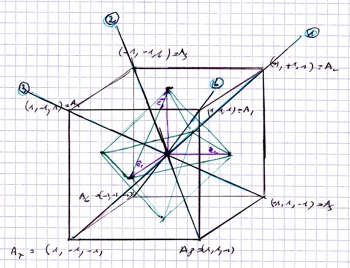
\includegraphics [width=12cm, height=10cm]  {octaedre.png}
\end{center}
\end{figure}

The cube of the centers of the faces of $S$ is a dilatation of a cube whose vertices are the points $(\pm 1, \pm1,\pm1)$, 
\begin{align*}
&A_1 = (1,1,1),A_2=(-1,1,1),A_3=(-1,-1,1),A_4=(1,-1,1),\\
&A_5=(-1,1,-1),A_6=(-1,-1,-1),A_7=(1,-1,-1),A_8=(1,1,-1).
\end{align*}

We give an arbitrary numbering of the four long diagonals:
\begin{align*}
D_1 &= A_2A_7, D_2=A_3A_8,
D_3=A_4A_5,D_4 =A_1A_6.
\end{align*}

The rotation $r_1 = \mathrm{Rot}(\pi, \overrightarrow{e_1})$ exchanges $A_4$ and $A_8$, and also $A_2$ and $A_6$,  thus exchanges $D_3$ with $D_2 $, $D_1$ with $D_4$ :
$$\varphi(r_1) = (1 4)(2 3).$$


$r_2 = \mathrm{Rot}(\pi/2, \overrightarrow{e_3})$ gives the cycle $A_1 \mapsto A_2\mapsto A_3 \mapsto A_4\mapsto A_1$, thus $D_1 \mapsto D_2 \mapsto D_3 \mapsto D_4 \mapsto D_1$ :
$$\varphi(r_2) = (1 2 3 4).$$


$r_3 = \mathrm{Rot}(\pi/2, \overrightarrow{e_2})$ v�rifie $A_1 \mapsto A_8 \mapsto A_5 \mapsto A_2\mapsto A_1$, thus $D_1 \mapsto D_4 \mapsto D_2 \mapsto D_3 \mapsto D_1$:

$$\varphi(r_3) = (1 4 2 3).$$

\item[(e)] Let $H = \langle (1 4)(2 3), (1 2 3 4), (1 4 2 3) \rangle \subset S_4$.

$H$ contains $[(1 4)(2 3)] \circ (1 2 3 4 ) = (1 3)$. Moreover the two permutations $(1 3) = ( 3 1), (1 4 2 3) = (3 1 4 2)$ generate $S_4$, since $(a_1 a_2), (a_1 a_2 \cdots a_n)$ generate $S_n$ genrally. Thus $H = G$:
$$S_4 = \langle \varphi(r_1), \varphi(r_2), \varphi(r_3) \rangle.$$

\item[(f)] 
As the subgroup $\varphi(G)$ contains $\varphi(r_1), \varphi(r_2), \varphi(r_3)$, it contains $S_4 = \langle \varphi(r_1), \varphi(r_2), \varphi(r_3) \rangle$. Therefore
$$\varphi(G) = S_4.$$
So $\varphi : G \to S_4$ is surjective. Moreover $\vert G \vert = \vert S_4 \vert = 24$, so $\varphi$ is bijective, $\varphi :G \to S_4$ is so an isomorphism.
$$G \simeq S_4.$$

As $\varphi(G) = \langle \varphi(r_1), \varphi(r_2), \varphi(r_3) \rangle$, where $\varphi$  is an isomorphism,
$$G = \langle r_1,r_2,r_3 \rangle.$$
\end{enumerate}
\end{proof}

\paragraph{Ex. 7.5.11}

{\it In this exercise, you will represent $\mathrm{AGL}(1,F)$ as a subgroup of $\mathrm{PGL}(2,F)$.
\be
\item[(a)] Show that the map $\gamma_{a,b} \mapsto  \left[
\begin{array}{ccc}
 a &   b   \\
  0&   1      
\end{array}
\right] $

defines a one-to-one group homomorphism
$$\mathrm{AGL}(1,F) \to \mathrm{PGL}(2,F).$$
\item[(b)] Consider the action of $\, \mathrm{PGL}(2,F)$ on $\hat{F}$. Show that the isotropy subgroup of $\mathrm{PGL}(2,F)$ acting on $\infty$ is the image of the homomorphism of part (a).
\ee
}


\begin{proof}
\begin{enumerate}
\item[(a)]
Write
$\gamma_{a,b} : F\to F,\  \alpha \mapsto \gamma_{a,b}(\alpha) = a\alpha+b$.
For all $\alpha \in F,$

$(\gamma_{a,b} \circ \gamma_{c,d})(\alpha) = a(c\alpha+d)+b=ac \alpha +ad+b = \gamma_{ac,ad+b}(\alpha)$, 

thus
$$\gamma_{a,b} \circ \gamma_{c,d} = \gamma_{ac,ad+b}.$$
Let 
$$
\varphi :
\left\{
\begin{array}{ccc}
 \mathrm{AGL}(1,F) &   \to & \mathrm{PGL}(2,F)  \\
  \gamma_{a,b}& \mapsto  &  \left[
\begin{array}{ccc}
 a &   b   \\
  0&   1      
\end{array}
\right] \\
\end{array}
 \right.
.
$$
\begin{align*}
\varphi(\gamma_{a,b}) \varphi( \gamma_{c,d}) &=
\left[
 \begin{array}{ccc}
 a &   b   \\
  0&   1      
\end{array}
\right] 
\left[
\begin{array}{ccc}
 c &   d   \\
  0&   1      
\end{array}
\right] \\
&=
\left[
\begin{array}{ccc}
 ac &   ad+b   \\
  0&   1      
\end{array}
\right] \\
&=\varphi( \gamma_{ac,ad+b})\\
&=\varphi(\gamma_{a,b} \circ \gamma_{c,d}).
\end{align*}
$\varphi :  \mathrm{AGL}(1,F)    \to  \mathrm{PGL}(2,F)$ is so a group homomorphism.
\begin{align*}
\gamma_{a,b} \in \ker(\varphi)& \iff 
\left[
 \begin{array}{ccc}
 a &   b   \\
  0&   1      
\end{array}
\right] =[I_2]\\
& \iff 
\left(
 \begin{array}{ccc}
 a &   b   \\
  0&   1      
\end{array}
\right) = 
\left(
 \begin{array}{ccc}
 \lambda&   0   \\
  0&   \lambda      
\end{array}
\right),
\ \lambda \in F^*\\
&\iff a=1, b=0\\
&\iff \gamma_{a,b} = 1_F
\end{align*}
$\ker(\varphi) = \{1_F\}$, thus $\varphi$ is an injective group homomorphism, which embeds  $\mathrm{AGL}(1,F)$ in $ \mathrm{PGL}(2,F)$.

\item[(b)]
Write $G_\infty$ the stabilizer of $\infty$ in $ \mathrm{PGL}(2,F)$.
\begin{align*}
\left[
\begin{array}{ccc}
 a &   b   \\
  c&   d     
\end{array}
\right]  \in G_\infty &\iff
\left(
\begin{array}{ccc}
 a &   b   \\
  c&   d      
\end{array}
\right)
\left(
\begin{array}{c}
  1    \\
  0      
\end{array}
\right)
= \lambda
\left(
\begin{array}{c}
  1    \\
  0      
\end{array}
\right),\  \lambda \in F^*
 \\
 &\iff c=0
\end{align*}
Let  $\gamma  = \left(
 \begin{array}{ccc}
 r &   s  \\
  t&   u      
\end{array}
\right)\in \mathrm{GL}(2,F)$. If  $[\gamma] \in \varphi(\mathrm{AGL}(1,F))$, then $[\gamma] =\varphi(\gamma_{a,b})= \left[
 \begin{array}{ccc}
 a&   b   \\
  0&   1      
\end{array}
\right]$, 
thus $[\gamma] \in G_\infty$ by the preceding equivalence.

Conversely, if $[\gamma] \in G_{\infty}$, then $t=0$, therefore $\det(\gamma) = ru \neq 0$, so $u \neq 0$.

$ 
\left(
\begin{array}{ccc}
 r &   s  \\
  t&   u      
\end{array}
\right) = u 
\left(
\begin{array}{ccc}
 r /u&   s/u  \\
  0&   1     
\end{array}
\right), \ u \in F^* 
$, thus $[\gamma] = 
\left[
 \begin{array}{ccc}
 a&   b   \\
  0&   1      
\end{array}
\right]$, where $a=r/u, b=s/u$ :
$[\gamma] = \varphi(\gamma_{a,b}) \in \varphi(\mathrm{AGL}(1,F))$.

$$G_\infty = \varphi( \mathrm{AGL}(1,F) ).$$

So $\mathrm{AGL}(1,F)$ is identified with the stabilizer of $\infty$ in $\mathrm{PGL}(2,F)$ and is isomorphic to a subgroup of $\mathrm{PGL}(2,F)$.
\end{enumerate}
\end{proof}

\paragraph{Ex. 7.5.12}

{\it In this exercise, you will construct polyhedra whose symmetry groups are isomorphic to $C_n$ and $D_{2n}$. For $D_{2n}$, consider the polyhedron whoss vertices are the north and south poles of $S^2$ together with the $n$th roots of unity along the equator (see picture in [D.Cox]). Note that to obtain a three dimensional object, we must assume $n\geq 3$.
\be
\item[(a)] Show that the symmetry group of this polyhedron is isomorphic to $D_{2n}$ when $n\neq 4$, and $S_4$ when $n = 4$.
\item[(b)] Now take the vertices on the equator and move them up in $S_2$ so that they become the vertice of a regular $n$-gone lying in the plane $z=c$, where $c>0$ is small. Prove that the symmetry group of this polyhedron is isomorphic to $C_n$.
\item[(c)] Find polyhedra inscribed in $S^2$ whose symmetry groups are $C_1$ (the trivial group), $C_2,D_4$ (the Klein four-group), and $D_8$ respectively.
\ee
}

\begin{proof}
\begin{enumerate}
\item[(a)]
Write $N,S$ the north and south poles, and $A_k$ the point of complex coordinate $\zeta_n^k$ in the equatorial plane. The polyhedron $P$ is the set of vertices
$$P = \{N,S,A_0,A_1,\cdots,A_{n-1}\}.$$
The group of symmetry of this polyhedron is 
$$G = G_P = \{ r \in \mathrm{SO}(3) \ \vert \ r(P) = P \}.$$

$G$ contains the rotation  $r = \mathrm{Rot}(\vec{e}_3,  2\pi/n)$ of axis $\vec{e}_3$ and angle $ 2\pi/n$, and also the rotation $s = \mathrm{Rot}(\vec{e}_1, \pi)$. So it contains the set $H = \{e,r,\cdots,r^{n-1}, s, rs,\cdots, r^{n-1}s\}$.

$$G \supset H = \{e,r,\cdots,r^{n-1}, s, rs,\cdots, r^{n-1}s\}.$$

The rotations $r^k = \mathrm{Rot}(\vec{e}_3,  2k\pi/n),\ k=0,\cdots,n-1$ send $A_0$ on $A_k$. So they are distinct  and they fix the poles, and the rotations $r^{n-1} \circ s$ are distinct and exchange the two poles, so are distinct of the $r^k$. Consequently $\vert H \vert = 2n$.
\begin{align*}
(r\circ s)(O) &= O = (s\circ r^{-1})(O), \\
(r \circ s)(P) &= S = (s\circ r^{-1})(P),\\
 (r\circ s)(A_0)&=A_1 = (s\circ r^{-1})(A_0),\\
 (r \circ s)(A_1) &= A_0 = (s\circ r^{-1})(A_1).
 \end{align*}
The 4 points $O,P,A_0,A_1$ are not coplanar, so form an affine frame, so the two rotations $r \circ s, s \circ r^{-1}$ gives the same image to the points of this frame are identical.

As $r$ is of order $n$, as $s$ is of order 2, and as $r\circ s=s\circ r^{-1}$, $H$ is a subgroup of $G$ isomorphic to the diedral group $D_{2n}$.

We show that if $n\neq 4, n\geq 3$, this inclusion is an equality.

Let $\rho \in G, \rho \neq e$, a rotation in $G$. $\rho$ fixes the gravity center $O$ of $P$, thus $\rho(O) = O$.

Write $A'_k = \rho(A_k)$.
As $\rho$ is an isometry, $A'_0 A'_1 = A_0A_1 = \vert \zeta_n-1 \vert$.


Moreover 
\begin{align*}
A'_0 A'_1 &= A_0A_1 = \vert \zeta_n-1 \vert =\vert e^{2i\pi/n} -1 \vert\\
&= \sqrt{\left(\cos \frac{2\pi}{n} - 1\right)^2 + \sin^2  \frac{2\pi}{n}}\\
&= \sqrt{2\left(1-\cos  \frac{2\pi}{n}\right)}\\
&=2 \sin  \frac{\pi}{n}
\end{align*}
(this can be proved geometrically).
Note that $P A_k = S A_k = \sqrt{2}$.

As $n\geq 3$,

$2 \sin \frac{\pi}{n} = 2$ is impossible since $\sin \frac{\pi}{n} \leq \sin \frac{\pi}{3} <1$.

$2 \sin  \frac{\pi}{n} =  \sqrt{2} \iff  \sin \frac{\pi}{n}  = \sin  \frac{\pi}{4} \iff n=4  $

Suppose that $n\neq 4$. With a reductio ad absurdum, if  $A'_0$ was a pole, then $A'_0A'_1 = \sqrt{2}$ (if $A'_1=A_k$) or $A'_0A'_1 = 2$ (if $A'_1$ is the opposite pole). In both cases, this is impossible, as previously proven.

Consequently $\rho(A_0) = A_k, \ k=0,1,\cdots,n-1$.
The same argument proves that the image of $A_i$ is in the polygon $\{A_0,,\cdots,A_{n-1}\}$, so $\rho$ is a permutation of the vertices of this polygon, thus sends $\{P,S\}$ sur $\{P,S\}$. Therefore$\rho$ fixes these two poles, or exchanges them.

\be
\item[$\bullet$] case 1: if $\rho(P) = P$, then since $\rho(O) = O, \rho(A_0)= A_k$, 
$\rho$ is the rotation $r^k = \mathrm{Rot}(\vec{e}_3,  2k\pi/n)$ of axis $OP$ ($1\leq k \leq n-1$), or the identity ($k=0$).


\item[$\bullet$] case 2 : if $\rho(P) = S$, then $(\rho \circ s)(P) = P$, and by case 1, $\rho \circ s = r^j, j=0,\cdots,n-1$, that is $\rho = r^j \circ s$.

\ee
In both cases, $\rho \in H$, therefore
$$G = H = \{e,r,\cdots,r^{n-1}, s, rs,\cdots, r^{n-1}s\} \simeq D_{2n}.$$

In the case $n=4$, we have proves in Exercise 10 that $G \simeq S_4$.

\item[(b)]
The modification of the polyhedron given in the text (or more simply the suppression of the south pole $S$) implies then $\rho(N) = N$, so it remains only the case 1 in the preceding discussion, so  $G = \langle r \rangle \simeq C_n$.

\item[(c)]
$\bullet$ The irregular tetrahedron  $T = \{(1,0,0), (0,1,0), (0,0,1), (\frac{1}{9},\frac{4}{9},\frac{8}{9})\}$, set of four non coplanar points 4,  est inscribed in $S_2$ (since $\left(\frac{1}{9}\right)^2 +\left(\frac{4}{9}\right)^2 +\left(\frac{8}{9}\right)^2  = 1$) and its symmetry group ist $G_T = \{e\}\simeq C_1$.

$\bullet$ Complete an isosceles non equilateral triangle  in the equatorial plane by the two poles: 

$P = \{(1,0,0), (\frac{2}{5},-\frac{3}{5},0), (-\frac{2}{5},-\frac{3}{5},0),  (0,0,1), (0,0,-1)\}$ has the symmetry group $G_P= \langle s \rangle \simeq C_2$, o� $s = \mathrm{Rot}(\vec{e}_1,\pi)$.

$\bullet$ The rectangle in the equatorial plane is completed by the two poles:

$R = \{(\frac{4}{5},\frac{3}{5},0),(\frac{4}{5},-\frac{3}{5},0),(-\frac{4}{5},-\frac{3}{5},0),-(\frac{4}{5},\frac{3}{5},0), (0,0,1), (0,0,-1)\}$ has the symmetry group $G_R =\langle \sigma, \tau,\xi\rangle$, where $\sigma,\tau,\xi$ are the rotations of angles $\pi$ and axes $\vec{e}_1, \vec{e}_2,\vec{e}_2$. $G_R \simeq D_4$ is the Klein four-group. 

$\bullet$ Soit $C$ a rectangular parallelepiped with square basis  inscribed in the sphere $S_2$ :

$
C=\{ (\frac{4}{9},\frac{8}{9},\frac{1}{9}),(-\frac{4}{9},\frac{8}{9},\frac{1}{9}),(-\frac{4}{9},-\frac{8}{9},\frac{1}{9}),(\frac{4}{9},-\frac{8}{9},\frac{1}{9}),\\
 \ \ (\frac{4}{9},\frac{8}{9},-\frac{1}{9}),(-\frac{4}{9},\frac{8}{9},-\frac{1}{9}),(-\frac{4}{9},-\frac{8}{9},-\frac{1}{9}),(\frac{4}{9},-\frac{8}{9},-\frac{1}{9}) \}. 
$

The symmetry group of $C$ is $G_C =\langle r,s \rangle= \{e,r,r^2,r^2,s,rs,r^2s,r^3s\}$, where $r = \mathrm{Rot}(\vec{e}_3,\pi/2), s = \mathrm{Rot}(\vec{e}_1,\pi)$, so $G_C \simeq D_8$.
\end{enumerate}
\end{proof}

\end{document}